% !TeX program = xelatex
% /*
%  * ----------------------------------------------------------------------------
%  * "THE BEER-WARE LICENSE" (Revision 42):
%  * <michi.wieland@hotmail.com> wrote this file. As long as you retain this notice you
%  * can do whatever you want with this stuff. If we meet some day, and you think
%  * this stuff is worth it, you can buy me a beer in return. Michael Wieland
%  * ----------------------------------------------------------------------------
%  */

% ------- template start -------
\documentclass[
a4paper,
oneside,
10pt,
fleqn,
headsepline,
toc=listofnumbered, 
bibliography=totocnumbered]{scrartcl}

% deutsche Trennmuster etc.
\usepackage[T1]{fontenc}
\usepackage[utf8]{inputenc}
\usepackage[english, ngerman]{babel} % \selectlanguage{english} if  needed
\usepackage{lmodern} % use modern latin fonts
\usepackage{tabularx}
\usepackage{float}

% Custom commands
\newcommand{\AUTHOR}{J.Hürzeler, S.Moll, S.Dellsperger, J.Klaiber, M.Wieland}
\newcommand{\INSTITUTE}{Fachhochschule OST}
\newcommand{\GITHUB}{https://github.com/joshuabeny1999/ost-zusammenfassungen}
\newcommand{\LICENSEURL}{https://en.wikipedia.org/wiki/Beerware}
\newcommand{\LICENSE}{
"THE BEER-WARE LICENSE" (Revision 42):
Joshua, Sharon, Severin, Julian and Michael wrote this file. As long as you retain this notice you
can do whatever you want with this stuff. If we meet some day, and you think
this stuff is worth it, you can buy us a beer in return.
}

% Jede Überschrift 1 auf neuer Seite
\let\stdsection\section
\renewcommand\section{\clearpage\stdsection}

% Multiple Authors
\usepackage{authblk}

% Include external pdf
\usepackage{pdfpages}

% Layout / Seitenränder
\usepackage{geometry}

% Inhaltsverzeichnis
\usepackage{makeidx} 
\makeindex

\usepackage{url}
\usepackage[pdfborder={0 0 0}]{hyperref}
\usepackage[all]{hypcap}
\usepackage{hyperxmp} % for license metadata

% Glossar und Abkürzungsverzeichnis
\usepackage[acronym,toc,nopostdot]{glossaries}
\setglossarystyle{altlist}
\usepackage{xparse}
\DeclareDocumentCommand{\newdualentry}{ O{} O{} m m m m } {
	\newglossaryentry{gls-#3}{
		name={#4 : #5},
		text={#5\glsadd{#3}},
		description={#6},
		#1
	}
	\makeglossaries
	\newacronym[see={[Siehe:]{gls-#3}},#2]{#3}{#4}{#5\glsadd{gls-#3}}
}
\makeglossaries

% Mathematik
\usepackage{amsmath}
\usepackage{amssymb}
\usepackage{amsfonts}
\usepackage{enumitem}

% Images
\usepackage{graphicx}
\graphicspath{{images/}} % default paths

% Boxes
\usepackage{fancybox}

%Tables
\usepackage{tabu}
\usepackage{booktabs} % toprule, midrule, bottomrule
\usepackage{array} % for matrix tables

% Multi Columns
\usepackage{multicol}

% Header and footer
\usepackage{scrlayer-scrpage}
\setkomafont{pagehead}{\normalfont}
\setkomafont{pagefoot}{\normalfont}
\automark*{section}
\clearpairofpagestyles
\ihead{\headmark}
\ohead{\AUTHOR}
\cfoot{\pagemark}

% Pseudocode
\usepackage{algorithmic}
\usepackage[linesnumbered,ruled]{algorithm2e}

% Code Listings
\usepackage{listings}
\usepackage{color}
\usepackage{beramono}

\definecolor{bluekeywords}{rgb}{0,0,1}
\definecolor{greencomments}{rgb}{0,0.5,0}
\definecolor{redstrings}{rgb}{0.64,0.08,0.08}
\definecolor{xmlcomments}{rgb}{0.5,0.5,0.5}
\definecolor{types}{rgb}{0.17,0.57,0.68}

\lstdefinestyle{visual-studio-style}{
	language=[Sharp]C,
	columns=flexible,
	showstringspaces=false,
	basicstyle=\footnotesize\ttfamily, 
	commentstyle=\color{greencomments},
	morekeywords={partial, var, value, get, set},
	keywordstyle=\bfseries\color{bluekeywords},
	stringstyle=\color{redstrings},
	breaklines=true,
	breakatwhitespace=true,
	tabsize=4,
	numbers=left,
	numberstyle=\tiny\color{black},
	frame=lines,
	showspaces=false,
	showtabs=false,
	escapeinside={£}{£},
}

\definecolor{DarkPurple}{rgb}{0.4, 0.1, 0.4}
\definecolor{DarkCyan}{rgb}{0.0, 0.5, 0.4}
\definecolor{LightLime}{rgb}{0.3, 0.5, 0.4}
\definecolor{Blue}{rgb}{0.0, 0.0, 1.0}

\lstdefinestyle{cevelop-style}{
	language=C++,  
	columns=flexible,
	showstringspaces=false,     
	basicstyle=\footnotesize\ttfamily, 
	keywordstyle=\bfseries\color{DarkPurple},
	commentstyle=\color{LightLime},
	stringstyle=\color{Blue}, 
	escapeinside={£}{£}, % latex scope within code      
	breaklines=true,
	breakatwhitespace=true,
	showspaces=false,
	showtabs=false,
	tabsize=4,
	morekeywords={include,ifndef,define},
	numbers=left,
	numberstyle=\tiny\color{black},
	frame=lines,
}

\lstdefinestyle{eclipse-style}{
	language=Java,  
	columns=flexible,
	showstringspaces=false,     
	basicstyle=\footnotesize\ttfamily, 
	keywordstyle=\bfseries\color{DarkPurple},
	commentstyle=\color{LightLime},
	stringstyle=\color{Blue}, 
	escapeinside={£}{£}, % latex scope within code      
	breaklines=true,
	breakatwhitespace=true,
	showspaces=false,
	showtabs=false,
	tabsize=4,
	morekeywords={length},
	numbers=left,
	numberstyle=\tiny\color{black},
	frame=lines,
}
\lstset{style=eclipse-style}



% Theorems \begin{mytheo}{title}{label}
\usepackage{tcolorbox}
\tcbuselibrary{theorems}
\newtcbtheorem[number within=section]{definiton}{Definition}%
{fonttitle=\bfseries}{def}
\newtcbtheorem[number within=section]{remember}{Merke}%
{fonttitle=\bfseries}{rem}
\newtcbtheorem[number within=section]{hint}{Hinweis}%
{fonttitle=\bfseries}{hnt}

% ------- template end -------

% Dokumentinformationen
\newcommand{\SUBJECT}{Zusammenfassung}
\newcommand{\TITLE}{Microsoft Technologien (.NET)}

\loadglsentries{glossar}

% ------- front start -------

% pdf metadata
\hypersetup{
	pdfauthor={\AUTHOR},
	pdftitle={\SUBJECT \TITLE},
	pdfcopyright={\LICENSE},
	pdflicenseurl={\LICENSEURL}
}

\begin{document}

% Front page
\title{\TITLE}
\subject{\SUBJECT}
\author{\AUTHOR}
\affil{\INSTITUTE}
\date{\today}
\maketitle

\vfill

% Licence
\paragraph{Lizenz} \hfill \\
\LICENSE

% Table of contents
\tableofcontents


% Glossar and acronyms (if included \loadglsentries{glossar})
\printglossary
\glsaddall

% ------- front end -------

\lstset{style=visual-studio-style}

\section{Der Heilige Gral}
\subsection{Reference oder Value}
\begin{itemize}
	\item Man unterscheidet zwischen Referenz- (Klassen) und Value Typen (Structs, Enum und primitive Datentypen)
	\item Bei Referenztypen liegt die Referenz auf dem Stack und das eigentliche Objekt auf dem Heap.
	\item Bei der Parameterübergabe bei Value wird eine Kopie angelegt. Bei Referenztypen wird einfach nur die Referenz auf dem Stack kopiert (nicht aber das Objekt!)
	\item Für die Parameterübergabe by Reference ist das Keyword \lstinline|ref| notwendig
	\item Ein \lstinline|out| Parameter verhält sich wie ein \lstinline|ref| Parameter, mit dem Unterschied, dass er nicht initialisiert sein muss.
	\item Strings werden auf dem Heap als \lstinline|char| Arrays alloziert.
	\item Boxing nennt man die automatische Umwandlung von einem Value in einen Referenz Type (implizit).
	\item Unboxing ist die automatische Umwandlung von einem Referent in einen Value Type (explizit).
\end{itemize}

\begin{minipage}[t]{0.9\textwidth}
	\centering
	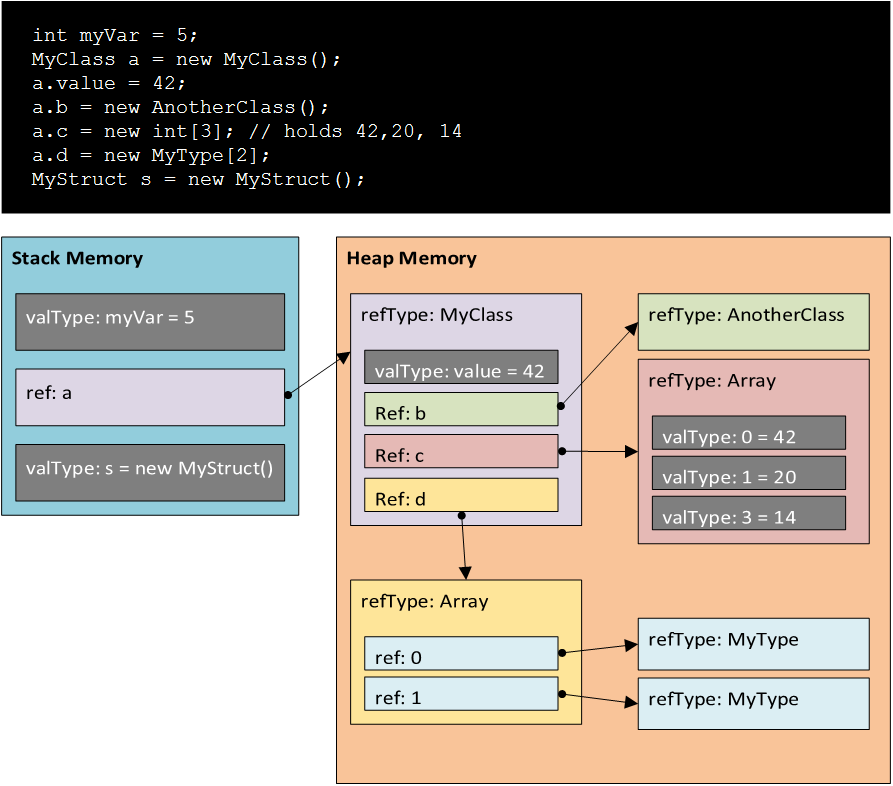
\includegraphics[width=0.8\linewidth]{images/reference_value_type}
\end{minipage}
\clearpage

\subsection{Lamdas}
\begin{itemize}
	\item Lamdas werden in \lstinline|Func<[param_type], [return _type]> myLamda;| gespeichert, wobei der letzte Typ in den spitzen Klammern der Rückgabe Typ ist.
\end{itemize}

\subsection{Delegates, Events}
Delegates sind typsichere Funktions-Pointer, wobei die Typsicherheit vom Compiler gewährleistet wird.
\begin{itemize}
	\item Der erste Parameter ist bei EventHandler immer immer das \lstinline|this| Objekt!
	\item In einem Event können mehrere Lamda/Funktionen registriert werden (+=)
	\item Wird ein Delegate in einer \lstinline|Func<T>| gespeichert kann das Delegate von überall verwendet werden. Das \lstinline|event| Keyword macht das Delegate privat und generiert public Methoden für die Registrierung und Deregistrierung.
\end{itemize}

\begin{lstlisting}
// defie event handler, where event happens (z.B Schalter)
public event EventHandler<MyEventArgs> MyEventHandler;
// define event args
public MyEventArgs : EventArgs {
	public string Value {get; set; }
}

// register a function to the event
// function is called, when event happens
MyEventHandler += (o, e) => {
	// do anything
}

// Invoke EventHandler
MyEventHandler?.Invoke(this, new MyEventArgs() {
	Value = "test"
});
\end{lstlisting}
\begin{lstlisting}
// without event args
public event Action<bool> MyEvent;
MyEvent?.Invoke(this, true);
// called function with bool param
public void EventHappens(bool state) { this.Light = state; }
MyEvent += Light.EventHappens; // register
\end{lstlisting}

\subsection{Extension Methods}
\begin{itemize}
	\item Eine Extension Method \textbf{und} die Wrapper Klasse müssen \lstinline|static| sein und der erste Parameter der Methode \lstinline|this| als Prefix haben.
	\item Der erste Parameter definiert die Klasse, welche erweitert wird
\end{itemize}

\begin{lstlisting}
using MyExtensions; // in callee

// simple iterator
public static class MyExtensions {
	public static IEnumerable<T> Ext1<T>(this IEnumerable<T> input) {
		 foreach (T item in input) {
			yield return item;
		}
	}
}
\end{lstlisting}

\clearpage

\subsection{LINQ}
\begin{itemize}
	\item Das Select Statement gibt ein Objekt vom Typ \lstinline|IEnumerable<T>| eines anonymen Types mit den jeweiligen Feldern zurück.
	\item Nützliche Funktionen sind \lstinline|g.Count()|, \lstinline|g.Average(e => e.Amount)|, \lstinline|g.Sum(e => e.Amout)|, \lstinline|x.Min(x => x.Price)|, \lstinline|x.Max(x => x.Price)|
\end{itemize}
\begin{lstlisting}
// extension syntax
var query = myArray
	.Where(e => e.Name.StartsWith("a") && e.Name.EndsWith("b"))
	.GroupBy(e => e.Department)
	.OrderBy(e => e.Name)
	.Select(e => new {
		Name = e.Name,
		Department = (e.Department == null) ? "empty" : e.Department
	})
	.ToList();

// query syntax
var query = from e in myArray
	from d in e.departments
	where e.StartsWith("a")
	group e by e.Name into mygroup [where mygroup.Count() > 3]
	orderby e.Name, d.Name // order by two fields
	select new {
		Name = mygroup.Key,
		Department = d.Name
	};
	
// inner join (==)
var innerJoinQuery =
    from c in categories
    join p in products on c.ID equals p.CategoryID // or compound 'from' over nav prop
    select new { 
	    ProductName = p.Name, 
	    Category = c.Name 
	};
	
// group join (into)
var innerGroupJoinQuery =
    from c in categories
    join p in products on c.ID equals p.CategoryID into prodGroup
    select new { 
	    CategoryName = c.Name, 
	    Products = prodGroup.Count()
	};
	
// left outer join (DefaultIfEmpty() combined with group join)
var leftOuterJoinQuery =
    from c in categories
    join p in products on c.ID equals p.CategoryID into prodGroup
    from item in prodGroup.DefaultIfEmpty(
	    new Product { // set default
		    Name = String.Empty, 
		    CategoryID = 0 
		})
    select new { 
	    CatName = c.Name, 
	    ProdName = item.Name 
	};
\end{lstlisting}

\clearpage

\subsection{Entity Framework}
\begin{itemize}
	\item Über den \lstinline|DbContext| findet die Kommunikation mit der Datenbank statt. Er ist für die Persistierung und Transaktionshandling verantwortlich. Jedes persistente Objekt ist dem DB Kontext zugeornet, was Caching und Tracking von Änderungen erlaubt.
	\item Der Entity Key ist die OO Representation des Primary/Foreign Key. Er wird vom DBContext gesetzt und hat beim Erzeugen den Default Wert seines Types. Sobald die OO Representation in der DB gespeichert wird, wird der Entity Key mit dem Primary Key aus der DB überschrieben.
	\item Für die Sicherstellung der referenziellen Integrität sind die Business Klasse selber zuständig.
	\item Das Entity Framework verwendet standardmässig \textbf{Lazy Loading}. Das bedeutet, dass die Daten erst geladen werden, wenn sie explizit dereferenziert werden. Die Navigation Property muss beim Lazy Loading \lstinline|virtual| sein!
	\item Beim \textbf{Eager Loading} wird das komplette Objekt mit einer \lstinline|Include("A.B")| Anweisung geladen.
\end{itemize}

\begin{lstlisting}
// lazy loading (navigation property needs to be virtual)
public class Blog  {  
	public int BlogId { get; set; }  
	public string Name { get; set; }  
	public string Url { get; set; }  
	public string Tags { get; set; }  
	
	// allows lazy loading
	public virtual ICollection<Post> Posts { get; set; }  
}

// eager loading (load everything at one using Include())
using (var context = new BloggingContext())  {
	var blogs1 = context.Blogs 
		 .Include(b => b.Posts) 
		 .ToList(); 
	
	var blogs2 = context.Blogs 
		 .Include("Posts") 
		 .ToList();
}

// disable lazy loading globally
public BloggingContext() { 
	this.Configuration.LazyLoadingEnabled = false; 
} 
\end{lstlisting}

\clearpage

\subsection{WCF}
\begin{itemize}
	\item Client und Server müssen das gleiche Binding haben. Dieses wird über den Metadata Exchange publiziert (MEX).
	\item Standardmässig werden alle public Properties/Felder eines DTO nach einander serialisiert.
	\item Der Service kann entweder direkt im Code im im XML definiert werden.
	\item Der Client kommuniziert immer über einen Proxy mit dem Service. Der Proxy kann generiert werden (Properties werden in Getter,Setter gewandelt, Listen Typinformationen gehen verloren)
\end{itemize}

\subsubsection{Server}
\begin{lstlisting}[caption=Data Transfer Objects (DTO)]
[DataContract]
[KnownType(typeof(DerivedA))]
[KnownType(typeof(DerivedB))]
public class AModelClass {
	[DataMember]
	public string Name {get; set;}	
}

[DataContract]
public class DerivedA : AModelClass {
	[DataMember]
	public string Name {get; set;}
}

[DataContract]
public class DerivedB : AModelClass, IInterface {
	[DataMember]
	public string Name {get; set;}
}

[DataContract]
public enum MyEnum {
	[EnumMember]
	A,
	[EnumMember]
	Bs
}
\end{lstlisting}
\begin{lstlisting}[caption=Service Interface]
// (may without callback)
[ServiceContract(
	CallbackContract=typeof(IMyCallback),
	SessionMode=SessionMode.Allowed)]
public interface IMyServiceInterface {
	List<AModelClass> Models {
		[OperationalContract[IsOneWay=false]]
		get;
	}
	
	[OperationContract]
	void GetModelById(int id);
	
	[ServiceKnownType(typeof(DerivedB))]
	[OperationContract]
	List<IInterface> getDerivedB();
}

// Callback Interface
public interface IMyCallback {
	[OperationContract(IsOneWay=true)]
	void PassResult(AModelClass model, bool success);
}

\end{lstlisting}
\begin{lstlisting}[caption=Service Implementation]
// Service Implementierung
[ServiceBehaviour(InstanceContextMode=InstanceContextMode.Single)]
public class MyService : IMyServiceInterface {
	private IMyCallback callback = ...;
	private List<AModelClass> models = new List<Models>();
	public List<AModelClass> Models {
		get { return models; }
	}
	
	public void GetModelById(int id) {
		Model model = models.Where(m => m.id = id);
		callback.PassResult(model, true);
	}
	
	public List<IInterface> getDerivedB() {
		return new List<DerivedB>();
	}
}

\end{lstlisting}
\begin{lstlisting}
// Usage (immer die Klasse, nie das Interface!)
ServiceHost myHost = new ServiceHost(typeof([namespace].MyService))
\end{lstlisting}

\begin{lstlisting}[caption=Service Hosting via XML]
<services>
	<service name="[namespace].MyService">
		 <!-- Endpoint: http://localhost:8732/MyService/ -->
		<endpoint address="" binding="basicHttpBinding" contract="[namespace].IMyServiceInterface"/>
		<!-- Endpoint: http://localhost:8732/MyService/mex -->
		<endpoint address="mex" binding="mexHttpBinding"  contract="IMetadataExchange"/> 
		<host>
			<baseAddresses>
				<add baseAddress="http://localhost:8732/MyService/"/>
			</baseAddresses>
		</host>
	</service>
</services>
\end{lstlisting}

\clearpage

\begin{lstlisting}[caption=Service Hosting via Code]
Uri address = new Uri("http://localhost:8732/MyService");
BasicHttpBinding binding = new BasicHttpBinding();

using(ServiceHost host = new ServiceHost(typeof([namespace].MyService), address)) {
	host.AddServiceEndpoint(typeof([namespace].IMyServiceInterface), binding, address);
	host.Open();
	Console.WriteLine("Service ready");
}
\end{lstlisting}

\subsubsection{Client}
\begin{lstlisting}
// name must match with xml name
var factory = new ChannelFactory<IMyServiceInterface>("MyService");
IMyServiceInterface proxy = factory.CreateChannel();
// use
proxy.GetDerivedB();
\end{lstlisting}

\begin{lstlisting}
<xml? version="1.0"?>
<configuration>
	<system.serviceModel>
		<client>
			<endpoint
				address="http://localhost:8732/MyService"
				binding="basicHttpBidning"
				contract="[namespace].IMyServiceInterface"
				name="MyService" />
		</client>
	</system.serviceModel>
</configuration>
\end{lstlisting}

\section{.NET}
\begin{itemize}
	\item Es werden aktuell über 30 Sprachen unterstützt
	\item Der Source Code wird in die Microsoft Intermediate Language  (MSIL: Ähnlich wie Assembler, vergleichbar mit Java Bytecode) kompiliert
	\item Alle Sprachen nutzen das selbe Objektmodell und Bibliotheken
	      \begin{itemize}
		      \item gemeinsamer IL-Zwischencode
		      \item gemeinsames Typensystem (CTS)
		      \item gemeinsame Runtime (CLR)
		      \item gemeinsame Klassenbibliotheken.
		      \item Das CLS definiert Einschränkungen an interoperablen Schnittstellen
	      \end{itemize}
	\item Der Debugger unterstützt alle Sprachen (auch Cross-Language Debugging möglich)
\end{itemize}
\begin{figure}[ht]
	\centering
	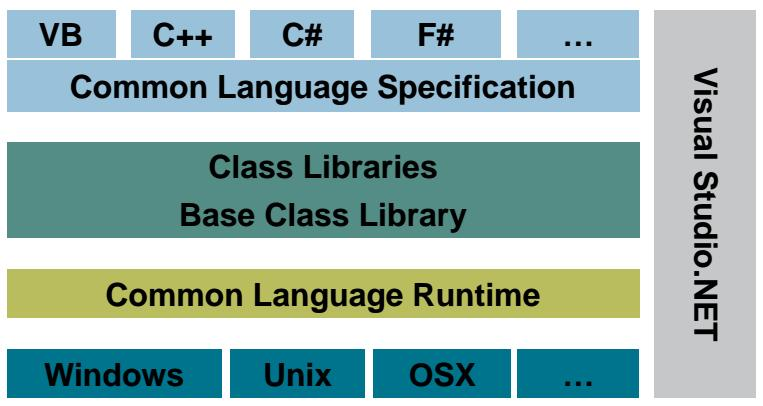
\includegraphics[width=0.6\linewidth]{images/net_framework_architektur}
	\caption{.NET Framework Architektur}
	\label{fig:netframeworkarchitektur}
\end{figure}

\subsection{CLR: Common Language Runtime}
Die \gls{clr} umfasst mehrere Funtionen wie z.B Just In Time Compilation für die Übersetzung von Intermediate Language Code in Maschinencode.Man versteht unter dem \gls{clr} ein sprachunabhängiges, abstrahiertes Betriebssystem. Es ist verantwortlich für das Memory Management, Class Loading, Garbage Collection, Exceptions, Type Checking, Code Verification des IL-Codes, Threadding
, Debugging und COM-Interopilität. Die CLR ist mit der Java VM vergleichbar.
\begin{figure}[ht]
	\centering
	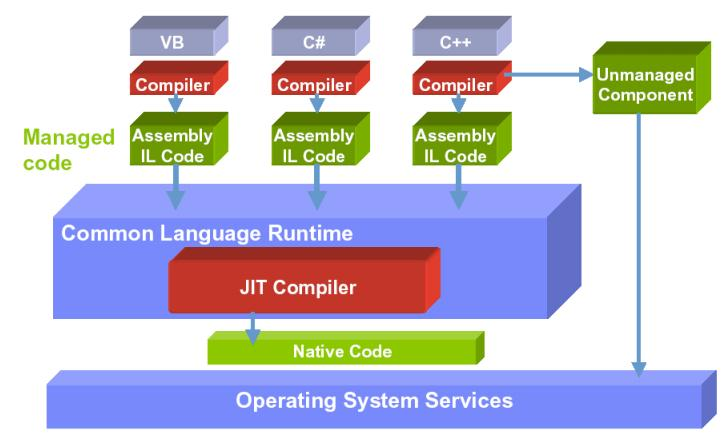
\includegraphics[width=0.6\linewidth]{images/common_language_runtime_architektur}
	\caption{CLR: Common Language Runtime Architektur}
	\label{fig:commonlanguageruntimearchitektur}
\end{figure}

\subsection{CTS: Common Type System}
Das \gls{cts} ist ein einheitliches Typensystem für alle .NET Programmiersprachen. \gls{cts} ist integriert in \gls{clr}.Mittels Reflection ist ein programmatisches abfragen des Typensystems möglich. (Erwieterbar mittels "Custom Attributes")

\subsection{CLS: Common Language Specification}
Die \gls{cls} sind allgemeine Regeln für die sprachübergreifende Entwicklung im .NET Framework. CLS kompatible Bibliotheken können in allen .NET Sprachen verwendet werden.

\subsection{MSIL: Microsoft Intermediate Language}
\gls{msil} ist eine \textbf{prozessor-, und sparchunabhängige} Zwischensprache die Assembler ähnelt.
\begin{enumerate}
	\item Sprachspezifischer Kompilier kompiliert nach MSIL
	\item \gls{jit} Compiler aus dem \gls{clr} kompiliert in nativen plattformabhängigen Code
\end{enumerate}
\paragraph{Vorteile}
\begin{itemize}
	\item Portabilität
	\item Typsicherheit: Beim Laden des Codes können Typensicherheits und Security Checks durchgeführt werden.
\end{itemize}
\paragraph{Nachteile}
\begin{itemize}
	\item Performance (kann verbessert werden, wenn JIT Compiler prozessorabhängige Hardwarebeschleunigung nutzt.)
\end{itemize}

\begin{figure}[ht]
	\centering
	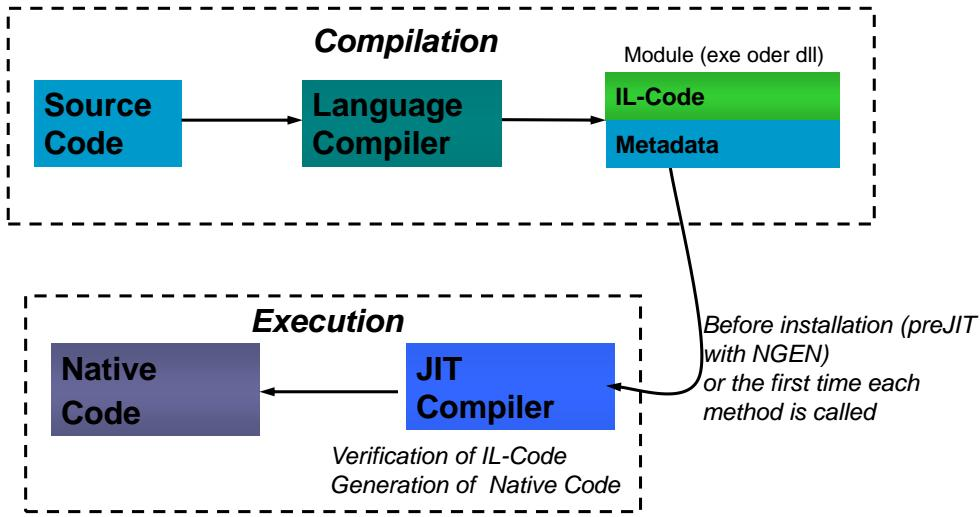
\includegraphics[width=0.7\linewidth]{images/msil_compilation}
	\caption{MSIL Kompilierung}
	\label{fig:msilcompilation}
\end{figure}

\subsection{JIT: Just in Time Compilation}
Bei der JIT Kompilierung wird die aufgerufene Methode vor dem Methodenaufruf kompiliert und der IL-Code durch nativen Code ersetzt. Es gibt drei Typen von JIT-Compilern:
\begin{itemize}
	\item Pre-JIT: Gesamter Code vor Ausführung (z.B mit NGEN)
	\item Normal-JIT (Siehe Diagramm)
	\item Econo-JIT: Wie Normal-JIT, aber mit Cleanup.
\end{itemize}

\subsection{Assembly / Komponenten}
\begin{figure}[!ht]
	\centering
	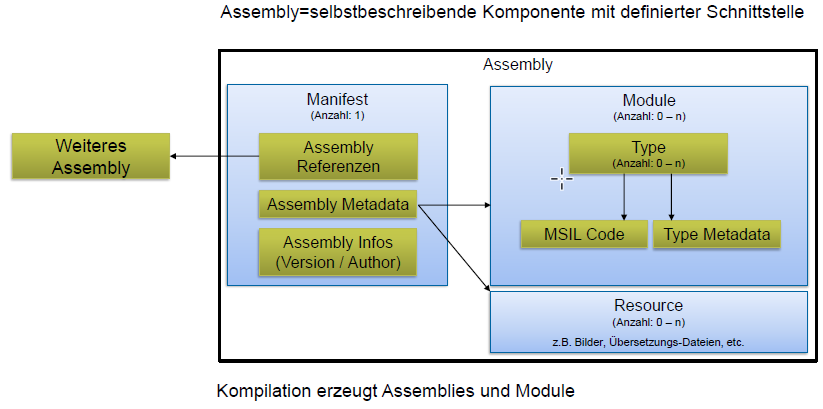
\includegraphics[width=0.9\linewidth]{images/assembly}
	\caption{Assembly Übersicht}
	\label{fig:assembly}
\end{figure}

Ein Assembly kann mit einem JAR File verglichen werden. Ein Assembly enthält MSIL-Code, Typ und Assembly Metadaten, Manifest mit strong names (Version/Author) und Referenzen auf andere Assemblies. Ein Assembly \textbf{kann aus mehreren Modulen bestehen}, \textbf{standardmässig} enthält ein Assembly aber \textbf{genau ein Modul}. Assemblies können nicht geschachtelt werden!
\begin{description}
	\item[Private Assembly] Private Assembly werden über einen Dateipfad referenziert und sind ansonsten nirgends registriert. Sie werden meist nur von einer Applikation genutzt.
	\item[Shared Assembly] Shared Assemblies verfügen über einen Strong Name (eindeutige Bezeichnung: Bez, Version, Culture, Public Key) und liegen im Global Assembly Cache (GAC). Ein Shared Assembly steht allen Applikationen zur Verfügung. Es sollte nicht zu viele Versionen im GAC registriert werden. (DLL Hell). Für die registriert wird das Command Line Tool \lstinline|gacutil.exe| verwendet.
\end{description}

\subsubsection{Module}
Die Kompilation erzeugt ein Modul mit Code / \gls{msil} und Metadaten. Die Metadaten beschreiben alle Aspekte des Codes ausser der Programmlogik. (Klassen, Methoden und Feld Definitonen) Diese Metadaten können mit Reflektion abgefragt werden. Die Metadaten werden von Analysetools (IL Dissassemlber), IDEs (IntelliSense, Object-Browser) als auch von der CLR (Typsicherheitverifikation, Memory Management, JIT Compilation) verwendet.

\subsubsection{References}
Referenzen zeigen auf eine externe Library. \\
Referenzen werden beim CSC mittels \lstinline|csc /target:exe /r:MyDLL.dll Program.cs| eingefügt. Es gibt verschiedene Arten:
\begin{itemize}
	\item Vorkompiliertes Assembly
	      \begin{itemize}
		      \item Im File System
		      \item Debugging nicht verfügbar
		      \item Navigation nur auf Metadaten-Ebenen
	      \end{itemize}
	\item NuGet package
	      \begin{itemize}
		      \item Externe Dependency (nuget.org)
		      \item Debugging nicht verfügbar
		      \item Navigation nur auf Metadaten-Ebenen
	      \end{itemize}
	\item Visual Studio Projekt
	      \begin{itemize}
		      \item In gleicher Solution vorhanden
		      \item Debugging und Navigation verfügbar
	      \end{itemize}
	\item .NET Core oder .NET Standard SDK
	      \begin{itemize}
		      \item Zwingend
		      \item Normalerweise: "Microsoft.NETCore.App"
		      \item Bei .NET Standard "NETStandard.Library"
	      \end{itemize}
\end{itemize}

\subsubsection{Packages}
.NET wird in kleineren Packages ausgeliefert und ist somit kein Monolitisches Framework mehr. Es wird aufgeteilt in diverse NuGet Packages. Dies erlaubt unterschiedliche Releasezyklen, erhöhung der Kompabilität und kleinere Deployment-Einheiten. Zu den wichtigen Packages gehören System.Runtime, System.Collections, System.Net.Http, System.IO.FileSystem, System.Linq und System.Reflection.
\paragraph{NuGet}\mbox{} \\
Die \lstinline|*.nupkg| Datei enthält alle Libaries in mehreren Versionen sowie die Manifest/Metadaten (Package Identifier, Titel, Beschreibung, Versions-Informationen, Dependencies, etc.). Es ist als Zip-Datei gespeichert.

Jeder kann Packages in der NuGet Gallery (www.nuget.org) veröffentlichen.
\clearpage

\subsection{Kompilierung}
Zur Kompilierung wird der \gls{csc} verwendet.
\begin{lstlisting}
// Create Executable: ClassA.exe
csc.exe /target:exe ClassA.cs

// Create Lib: ClassA.dll
csc.exe /target:library ClassA.cs

// Create Executable, referencing a Lib
csc.exe /target:exe
		/out:Programm.exe
		/r:ClassA.dll // or /r:System.Windows.Forms.dll (GAC)
		ClassB.cs ClassC.cs
// Ergibt = Program.exe
\end{lstlisting}

\subsection{Garbage Collection}
Der Garbage Collector löscht Objekte auf dem Heap, die nicht mehr über eine Root-Referenz referenziert werden. (Mark and Sweep) Wie in Java weiss man nicht wenn der GC aufgerufen wird (\textbf{nicht deterministisch}). Er kann aber mit der Methode GC.Collect() manuell aufgerufen werden. Der Ablauf ist immer gleich:
\begin{enumerate}
	\item Alle Objekte als Garbage betrachten
	\item Alle reachable Objekte markieren
	\item Alle nicht markierten Objete freigeben
	\item Speicher kompaktieren
\end{enumerate}

Die Garbage Collection started, sobald eine dieser Bedingungen wahr ist
\begin{itemize}
	\item System hat zu wenig Arbeitsspeicher
	\item Allozierte Objekte im Heap übersteigen einen Schwellwert
	\item GC.Collect Methode wird aufgerufen.
\end{itemize}

\paragraph{Root Referenzen}
Root-Referenzen sind statische Felder und aktive lokale Variablen auf dem Stack.

\subsubsection{Generationen}
Objekte werden in drei Generationen aufgeteilt: Zuerst werden die Objekte der 0ten Generation abgeräumt.
\begin{itemize}
	\item Generation 0: Objekte wurden seit dem letzten GC Durchlauf neu erstellt (z.B lokale Variablen)
	\item Generation 1: Objekte die einen GC Durchlauf überlebt haben (z.B Members)
	\item Generation 2: Objekte die mehr als einen GC Durchlauf überlebt haben.
\end{itemize}

\subsubsection{Deterministic Finalization} Objekte sollten wenn nötig mit dem Interface \lstinline|IDisposable| und der \lstinline|void Dispose()| Methode finalisiert werden und nur wenn nötig mit einem Destruktor. Man spricht von Deterministic Finalization, wenn der Programmierer für die Freigabe der unmanaged Ressourcen zuständig ist und diese explizit über \lstinline|Dispose()| freigibt. Dazu muss die \lstinline|Dispose()| Methode überschrieben werden. Mit \lstinline|using| wird der Aufrufe von \lstinline|Dispose()| implizit sichergestellt. Deterministic Finalization sollte bei allen I/O Klassen verwendet werden.
\begin{itemize}
	\item Dateisystem Zugriffe
	\item Netzwerk Kommunikation
	\item Datenbank Anbindung
\end{itemize}

\begin{lstlisting}
public class DataAccess : IDisposable {
	private DbConnection connection;
	public DataAccess() { 
		connection = new SqlConnection();
	}
	
	~DataAccess() {
		// backup
		connection.Dispose(); 
	}
	
	public void Dispose() {
		// supress GC, as we just want to call dispose
		System.GC.SuppressFinalize(this);
		connection.Dispose();
		// Call base.Dispose(); if necessary
	}
}

using (DataAccess dataAccess = new DataAccess()) {
	// work with dataAccess
}
\end{lstlisting}

\subsubsection{Finalizer} Der Gebrauch von herkömmlichen Finalizer ist nicht deterministisch (man weiss nicht wann der GC aufgerufen wird). Der Garbage Collector arbeitet viel effizienter wenn kein Destruktor/Finalizer vorhanden ist. Einflüsse auf den GC Aufruf sind folgende:
\begin{itemize}
	\item Gerade verfügbarem Speicher
	\item Generation des aktuellen Objektes
	\item Reihenfolge in der Finalization Queue
	\item Manuell oder automatisch getriggert
	\item Kann auch abhängig von der .NET Runtime Version sein
\end{itemize}

\subsubsection{Object Pinning} Der GC kompaktiert Speicher bei Bedarf. Mit dem Keyword \lstinline|fixed| kann dies unterbunden werden. (schlechte Performance)

\subsubsection{Weak References} Wird eine strong Referenz (default) auf null gesetzt, wird es irgendwann vom GC abgeräumt. Auf das null objekt kann nicht mehr zugegriffen werden. Mit Weak Refenzen kann man immer noch auf das Objekt zugreifen, bis es vom GC abgeräumt wird. Mit der Methode \lstinline|TryGetTarget(out sr)| kann man auf das alte Objekt zugreifen und dieses wiederherstellen. Wurde das Objekt abgeräumt, muss es neu erstellt werden.

\subsubsection{Memory Leaks} Memory Leaks entstehen, wenn z.B ein Event Listener nicht abgeräumt wird. Objekte welche aus einer anonymen Methode oder Lamda Ausdruck innerhalb eines Event Listener noch referenziert werden, werden nicht abgeräumt. Gleiches gilt für alle IDisposable Objekte, bei denen \lstinline|Dispose()| nicht aufgerufen wurde. (z.B DB Connection)

\begin{lstlisting}
// interface
public interface IDisposable {
	void Dispose();
}
	
// deterministic finalization
public class DataAccess : IDisposable {
		private DbConnection connection;
		public DataAccess() {
			connection = new SQLConnection();
		}
	
	~DataAccess() {
		connection.Dispose();
	}
	
	public void Dispose() {
		System.GC.SuppressFinalize(this);
		connection.Dispose();
	}
}

class MyClass {
	// call disposal
	DataAccess dataAccess = new DataAccess() ;
	dataAccess.Dispose();
	
	// implicit Disposal call with using
	// Multiple usings possible
	// syntactic sugar, compiles to try-finally with Dispose call
	using (DataAccess dataAccess = new DataAccess())
	using (SQLParser parser = new SQLParser()) {
		..
	}
	
	// or with same type
	using (DataAccess da1 = new DataAccess(), DataAccess da2 = new DataAccess()) {
		..
	}
}
\end{lstlisting}

\section{.NET Standard}
Der .NET Standard bietet die Brücke zwischen den ehemaligen Versionen .NET Framework (Windows) und .NET Core (Universal). Wobei es inzwichen nur noch .NET gibt. Es bietet die gemeinsamen Schnittstellen an, die bei beiden Versionen verwendet werden können. Es werden die minimal zu unterstützten APIs (Klassen und Methoden) pro Version definiert. Als Entwickler kann man sein package kompatibel zu einer bestimmten Standard Version machen. Diese Libaries sind dann Cross-Plattform. Man hält die Fragmentierung der Framework minimal und reduziert Pre-Compiler-Anweisungen.

\begin{figure}[!ht]
	\centering
	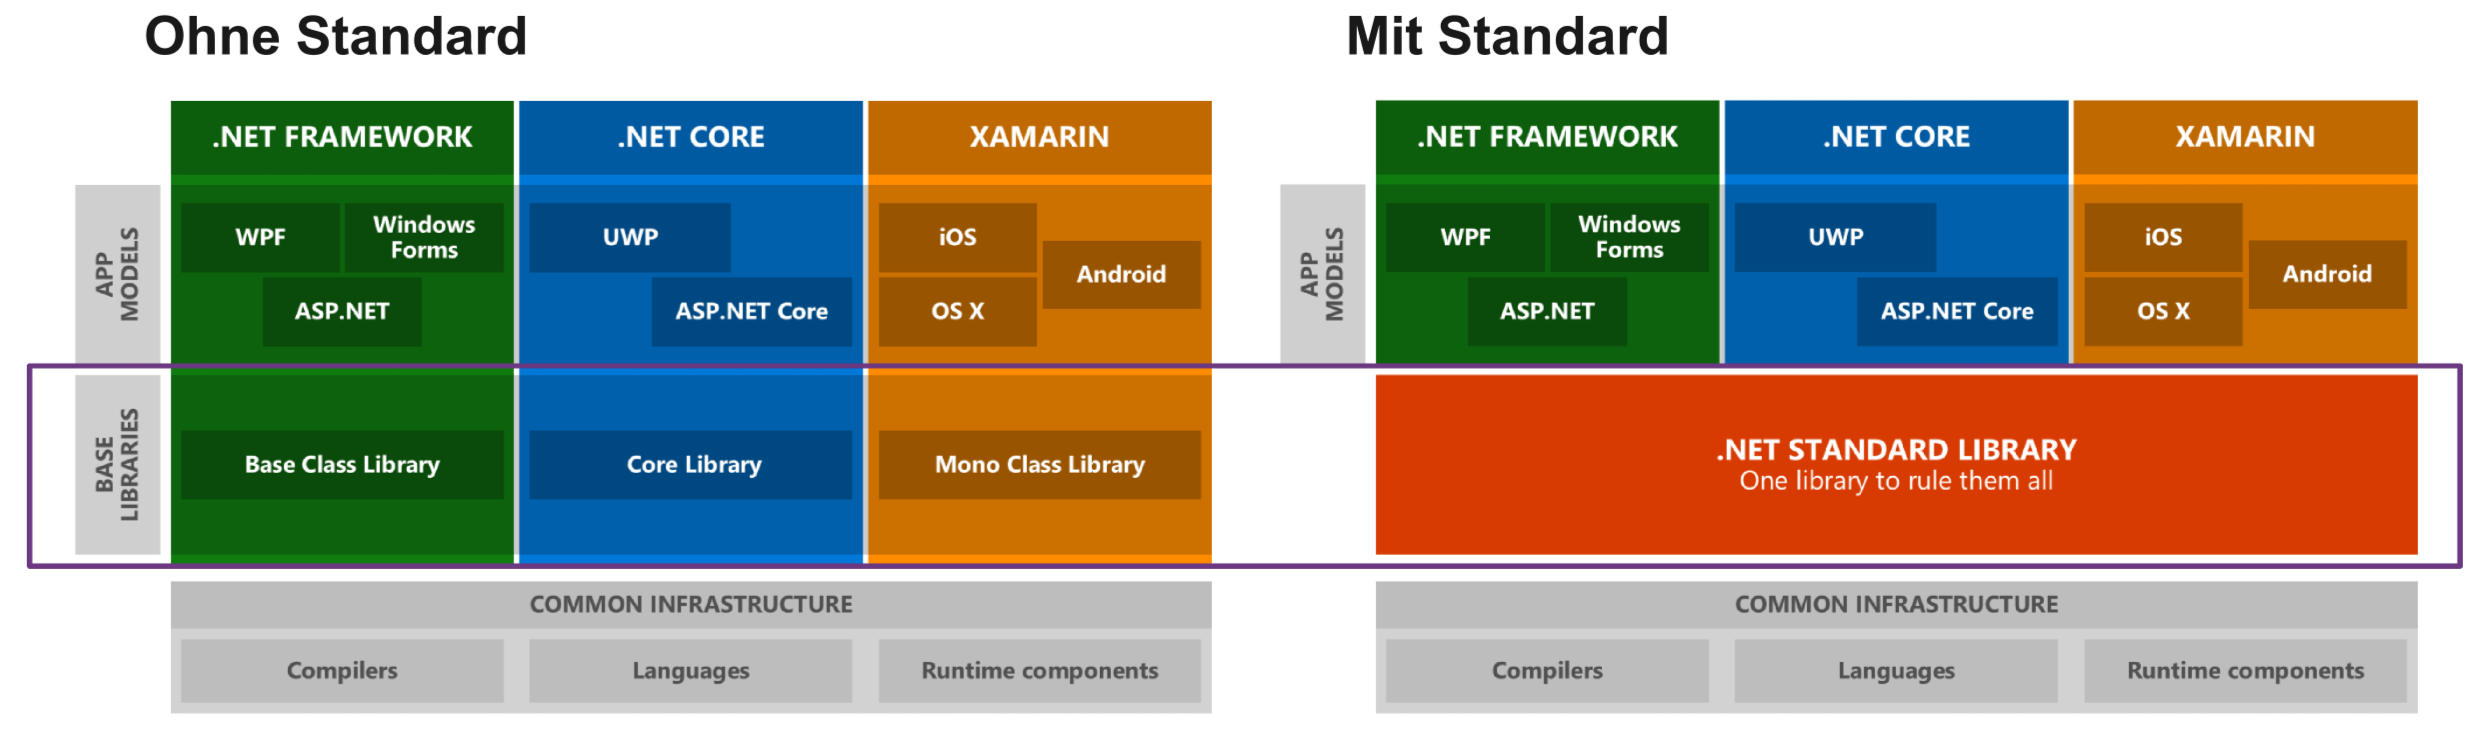
\includegraphics[width=1\linewidth]{images/standard-vergleich}
	\caption{Vergleich ohne und mit .NET Standard}
	\label{fig:standardvergleich}
\end{figure}

Je höher die Version desto mehr .NET Apis, desto tiefer, einfacher einzubinden. Jede .NET Implementation unterstützt eine andere maximale .NET Standard version. So wird beispielsweise .NET Standard 2.1 von .NET Framework nicht mehr supported, sondern nur noch von .NET Core 3.0 und .NET.
\begin{figure}[!ht]
	\centering
	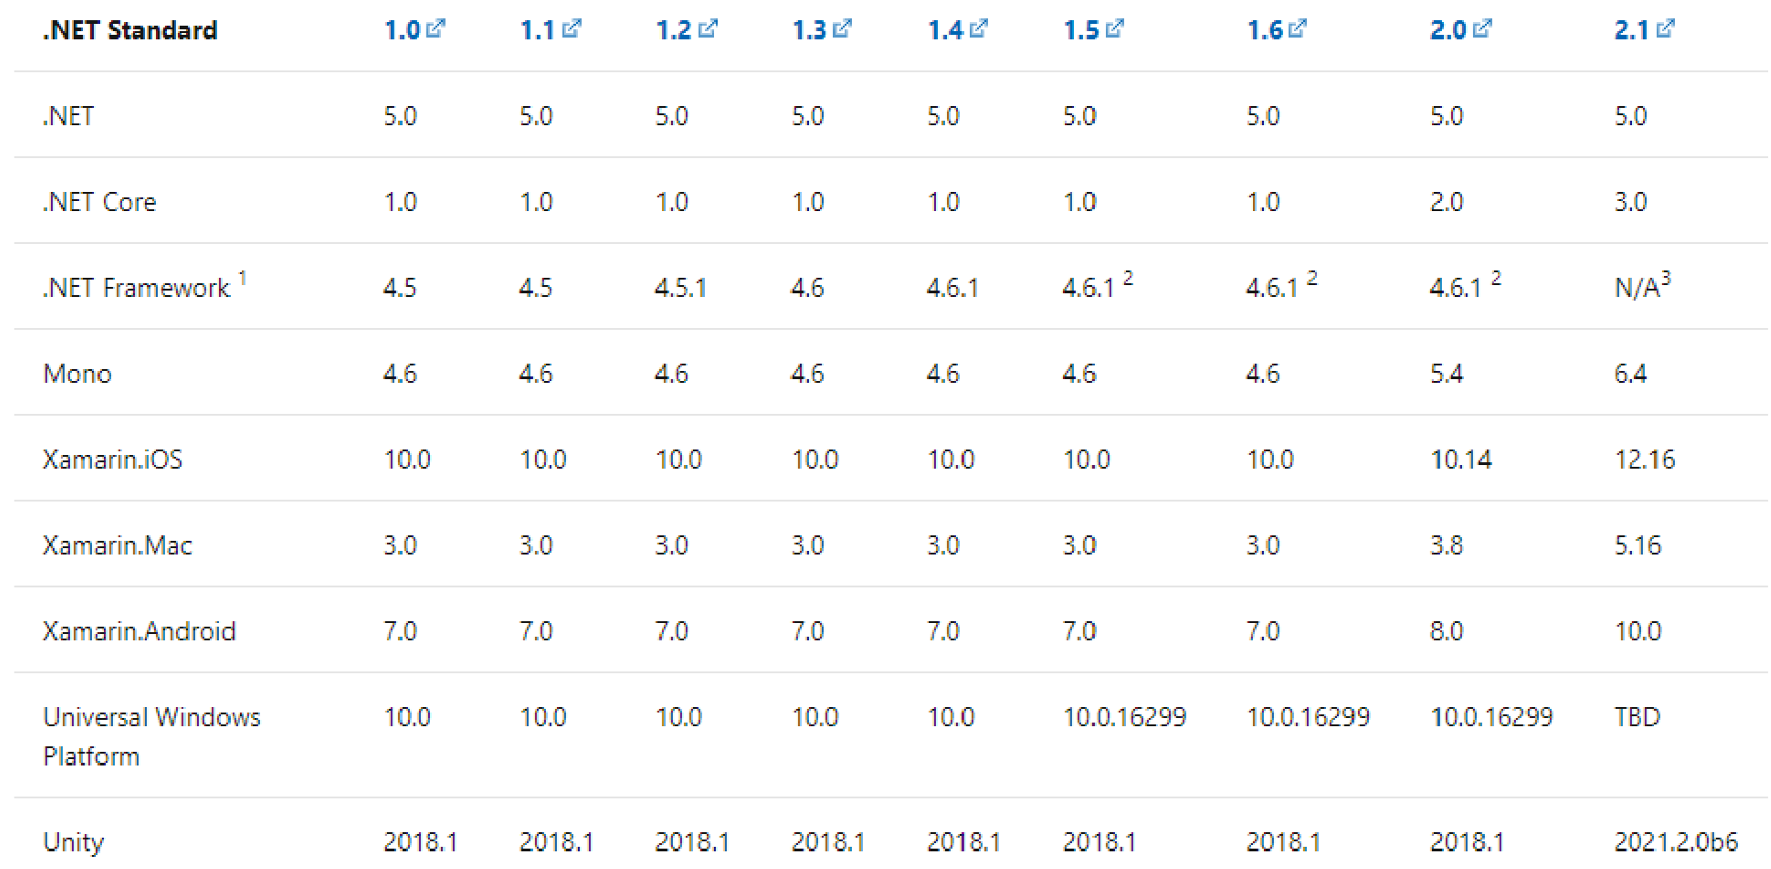
\includegraphics[width=0.9\linewidth]{images/standard-versionen}
	\caption{Übersicht der .NET-Implementation und deren kompatiblen .NET Standard Versionen}
	\label{fig:standardversionen}
\end{figure}
\section{Command Line Interface CLI}
Die CLI ist Teil des .NET Core SDK. Es ist die Basis für die high-level Tools (Visual Studio, Rider, etc.) Aufgerufen wird es mit \lstinline|dotnet[.exe] <Verb> <argument> --<option> <param>|.
\subsection{Kommandos}
\begin{description}
	\item[new] Initialize .NET projects.
	\item[restore] Restore dependencies specified in the .NET project.
	\item[run] Compiles and immediately executes a .NET project.
	\item[build] Builds a .NET project.
	\item[publish] Publishes a .NET project for deployment (including the runtime).
	\item[test] Runs unit tests using the test runner specified in the project.
	\item[pack] Creates a NuGet package.
	\item[migrate] Migrates a project.json based project to a msbuild based project.
	\item[clean] Clean build output(s).
	\item[sln] Modify solution (SLN) files.
	\item[add] Add reference to the project.
	\item[remove] Remove reference from the project.
	\item[list] List references of a .NET project.
	\item[nuget] Provides additional NuGet commands.
	\item[msbuild] Runs Microsoft Build Engine (MSBuild).
	\item[vstest] Runs Microsoft Test Execution Command Line Tool.
	\item[store] Stores the specified assemblies in the runtime store.
	\item[tool] Install or work with tools that extend the .NET experience.
	\item[build-server] Interact with servers started by a build.
	\item[help] Show help.
\end{description}


\section{Visual Studio 22}
\subsection{Solution}
Eine Solution besteht aus mehreren Projekten.

\subsection{Umbenennen}
Folgende Objekte müssen manuell umbenannt werden
\begin{itemize}
	\item Ordner in der das Projekt liegt
	      \begin{enumerate}
		      \item Manuelle Anpassung des Ordner Names in File-System
		      \item  Manuelles Anpassen der *.sln-Datei
	      \end{enumerate}
	\item Name des Assemblies
	      \begin{itemize}
		      \item Rechts-Klick auf Projekt > Properties > Application > Assembly name
	      \end{itemize}
	\item Name des Default Namespaces (wird bei neuen Classen verwendet)
	      \begin{itemize}
		      \item Rechts-Klick auf Projekt > Properties > Application > Default namespace
	      \end{itemize}
\end{itemize}

\subsection{Ordnerstruktur}
Jeder Projektordner enthält folgende zwei Verzeichnisse
\begin{description}
	\item[bin\textbackslash<BuildKonfiguration>] \hfill \\
		Beinhaltet das fertige, gelinkte Kompilat
	\item[obj\textbackslash<BuildKonfiguration>] \hfill \\
		Beihaltet Files welche während der Kompilierung erzeugt werden und für die Erstellung eines Assemblies nötig sind.
\end{description}

\subsection{Projekt-Dateien}
Die Projekte werden als XML-Datei verwaltet in einer \lstinline|*.csproj| Datei. Es beschreibt was alles Kompiliert werden muss, etc. Die Projektdateien werden von Build Engines intepretiert. Es gibt diverse Gruppen. Da gibt es Property-Groups (Settings), Item-Groups (Zu kompiliertende Items), Target-Groups (Weitere Buildsteps)

\section{C\# Grundlagen}
\subsection{Unterschiede zu Java}
\begin{itemize}
	\item Es gibt Structs, welche wie Klassen sind (jedoch Wertetypen)
	\item Es gibt Properties (spez. Getter und Setter) und Indexer (erweiterter Array Zugriff)
	\item Andere Syntax bei den Konstruktoren
	\item Es gibt Operator Overloading
	\item Parameterübergabe kann explizit by value oder by reference sein (auch für Wertetypen)
	\item Es gibt partielle Klassen und Methoden für Generatoren
	\item Es heisst \lstinline|NullReferenceException| und nicht \lstinline|NullPointerException|
	\item Es heisst \lstinline|base| und nicht \lstinline|super|
	\item Konstruktorparameter können direkt dem Parent übergeben werden. (\lstinline|public Derived(int x) : base(x) { .. }|)
\end{itemize}

\subsection{Naming Conventions}
\begin{table}[ht]
	\centering
	\begin{tabu} to \linewidth {l l l}
		\toprule
		Element        & Casing     & Beispiel                   \\
		\midrule
		Namespace      & PascalCase & System.Collections.Generic \\
		Klasse, Struct & PascalCase & BackColor                  \\
		Interface      & PascalCase & IComparable                \\
		Enum           & PascalCase & Color                      \\
		Delegates      & PascalCase & Action / Func              \\
		Methoden       & PascalCase & GetDataRow, UpdateOrder    \\
		Felder         & CamelCase  & name, orderId              \\
		Properties     & PascalCase & OrderId                    \\
		Events         & PascalCase & MouseClick                 \\
		\bottomrule
	\end{tabu}
	\caption{Naming Conventions}
\end{table}

\subsection{Sichtbarkeiten}
\begin{itemize}
	\item Abgeleitete Klasse/Interfaces dürfen nicht die grössere Sichtbarkeit als ihren Basistyp haben (z.B Parent ''internal'' und Sub ''public'')
	\item Member Typen müssen mindestens gleich sichtbar wie der Typ selbst sein
	\item Standad Sichtbarkeit ist \lstinline|internal|
	\item Interface Member dürfen keine Angaben zur Sichtbarkeit haben.
\end{itemize}
\begin{table}[ht]
	\centering
	\begin{tabu} to \linewidth {l l}
		\toprule
		Attribut           & Beschreibung                                                                                          \\
		\midrule
		public             & Überall sichtbar                                                                                      \\
		private            & Innerhalb des jeweiligen Typen sichtbar (Klasse/Struct)                                               \\
		protected          & Innerhalb des jeweiligen Typen oder abgeleiteten Klasse sichtbar (Klasse/Struct)                      \\
		internal           & Innerhalb des jeweiligen Assemblies sichtbar                                                          \\
		protected internal & Kombination aus internal und protected                                                                \\
		private protected* & Innerhalb des jeweiligen Typen oder abgeleiteter Klasse sichtbar, wenn diese im gleichem Assembly ist \\
		\bottomrule
	\end{tabu}
	\caption{Sichtbarkeiten}
\end{table}

\begin{table}[ht]
	\centering
	\begin{tabu} to \linewidth {l l l X}
		\toprule
		Typ       & Sichtbarkeit              & Member (default) & Member (zulässig)                                                           \\
		\midrule
		class     & public, internal(default) & private          & public, protected, internal, private, protected internal, private protected \\
		struct    & public, internal(default) & private          & public, internal, private                                                   \\
		enum      & public, internal(default) & public           & -                                                                           \\
		interface & public, internal(default) & public           & -                                                                           \\
		delegate  & public, internal(default) & -                & -                                                                           \\
		\bottomrule
	\end{tabu}
	\caption{Standard Sichtbarkeiten von Typen}
\end{table}

\newpage

\subsection{Operatoren}
\begin{figure}[!ht]
	\centering
	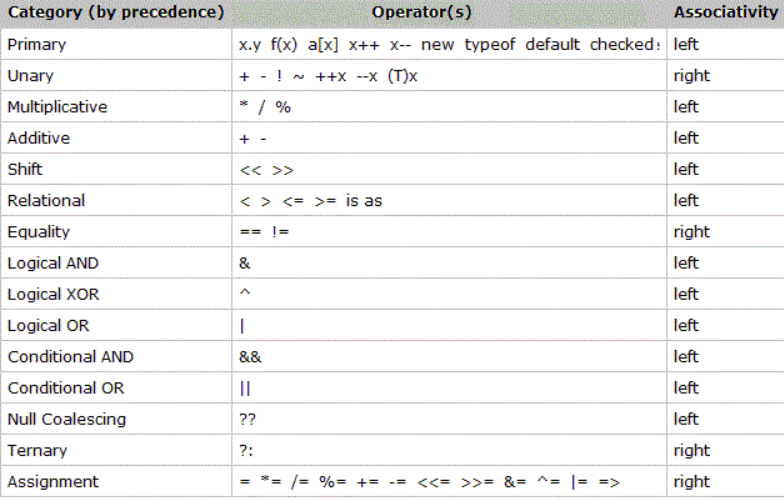
\includegraphics[width=\linewidth]{images/operator_prezedenz}
	\caption{Operatoren Präzedenz}
	\label{fig:operatorprezedenz}
\end{figure}

\clearpage

\subsection{Pre-, Post-Inkrmenet}
\begin{lstlisting}
// post increment
int a = 1;
int b = a++; // a=2, b=1

// pre increment
a = 1;
b = ++a; // a=2, b=2
\end{lstlisting}

\subsection{Statements}
\subsubsection{If Else If Else}
\begin{lstlisting}
if () {
} else if () {
} else {}
\end{lstlisting}

\subsubsection{Switch Case}
\begin{lstlisting}
switch() {
case:
case: break;
}
\end{lstlisting}

\subsubsection{Loops}
\begin{lstlisting}
while() {}
do {} while ();
for (int = 1; i <= myList.Count(); i++) {}
foreach(int x in y);
\end{lstlisting}

\subsubsection{Kommentare}
\begin{lstlisting}
// Single Line Comment
/* Multiline Comment */
/// Dokumentation
\end{lstlisting}

\clearpage

\subsection{Datentypen}
Numerische Datentypen können einen der folgenden Literale haben
\begin{figure}[!ht]
	\centering
	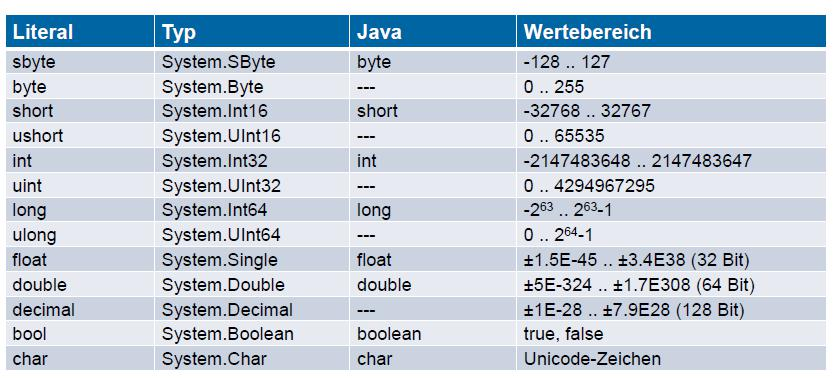
\includegraphics[width=0.8\linewidth]{images/primitive_types}
	\caption{Primitive Typen}
	\label{fig:primitivetypes}
\end{figure}

\begin{itemize}
	\item u/U: unsigned (signed Variablen können nur mit einem cast einer unsigned Variablen zugewiesen werden)
	\item l/L: long
	\item f/F: float
\end{itemize}
\begin{figure}[!ht]
	\centering
	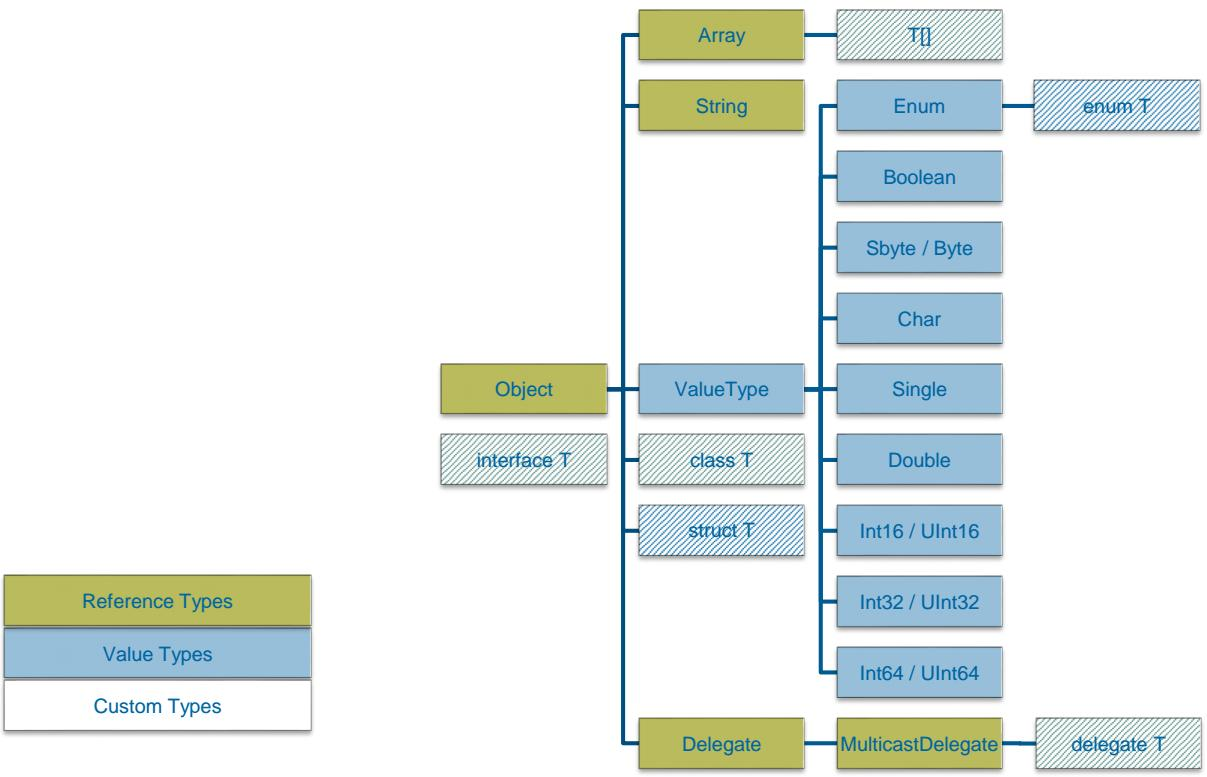
\includegraphics[width=0.8\linewidth]{images/datatypes}
	\caption{Datentypen}
	\label{fig:datatypes}
\end{figure}

\begin{figure}[!ht]
	\centering
	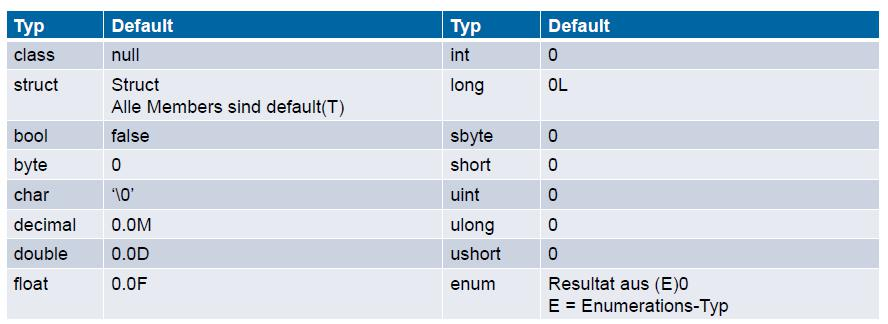
\includegraphics[width=\linewidth]{images/default_values}
	\caption{Default Values}
	\label{fig:defaultvalues}
\end{figure}

\newpage

\subsubsection{Casts}
\begin{figure}[!ht]
	\centering
	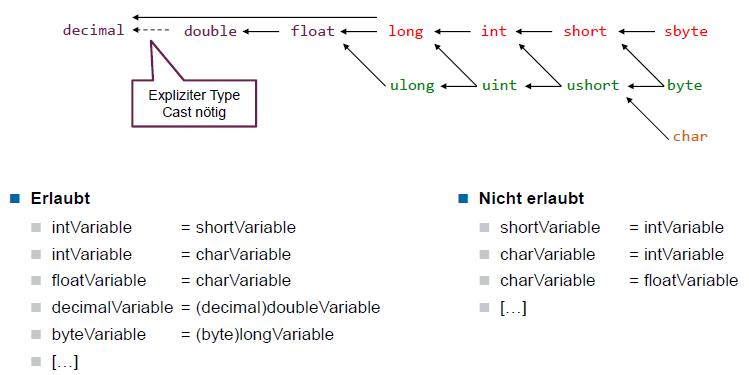
\includegraphics[width=\linewidth]{images/casts}
	\caption{Casts}
	\label{fig:casts}
\end{figure}

\clearpage

\subsubsection{Reference Types / Referenztypen}
\begin{itemize}
	\item Sind auf dem Heap gespeichert, wobei die Variable an sich auf dem Stack liegt
	\item Die Referenzen werden automatisch vom Garbage Collector aufgeräumt
	\item Wird ein Reference Type einer Methode übergeben, wird die Objekt referenz kopiert. (sofern nicht \lstinline|ref|)
\end{itemize}

\subsubsection{Value Types / Werttypen}
\begin{itemize}
	\item Sind auf dem Stack gespeichert
	\item Primitive Datentypen, Struct und System.Enum
	\item Wird eine Value Type Variable einer weiteren Value Type Variable zugewiesen, wird der Wert kopiert. Gleiches gilt für die Methodenparameter by Value.
\end{itemize}

\begin{figure}[ht!]
	\centering
	\begin{minipage}[t]{0.4\textwidth}
		\centering
		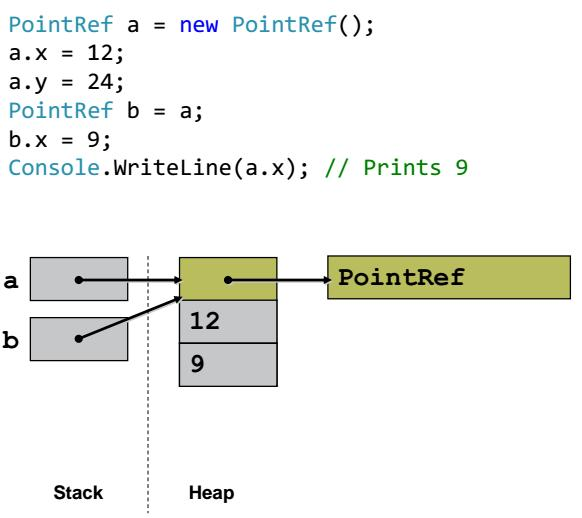
\includegraphics[width=0.8\linewidth]{images/reference_types}
		\captionof{figure}(Referenztypen)
		\label{fig:searchtreeinsert1}
	\end{minipage}
	\begin{minipage}[t]{0.4\textwidth}
		\centering
		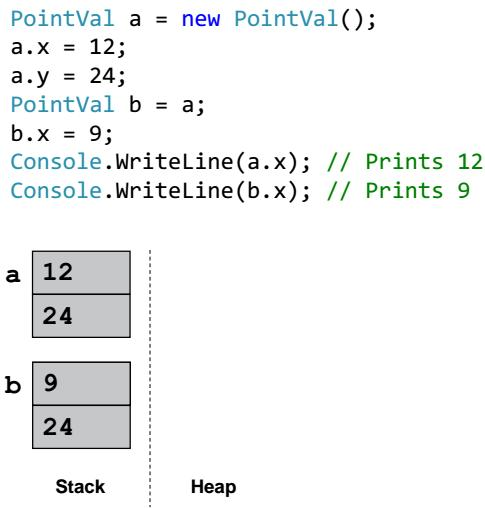
\includegraphics[width=0.8\linewidth]{images/value_types}
		\captionof{figure}(Wertetypen)
		\label{fig:searchtreeinsert2}
	\end{minipage}
\end{figure}

\clearpage

\subsection{Nullable Types}
\begin{itemize}
	\item Der ? Operator erlaubt es Null Werte einem Wertetyp zuzuweisen. Der Typ ist dann \lstinline|Nullable<T>|
	\item Arithmetisch Ausdrücke mit Null ergeben immer \lstinline|null|
	\item Vergleiche mit Null sind immer \lstinline|false|. Ausnahme \lstinline|null == null|
	\item Der ?? Operator erlaubt es einen Default Wert anzugeben, falls die Variable leer ist. Der zurückgegebene Typ ist dann kein Nullable-Type mehr(z.B \lstinline|int|)
\end{itemize}
\begin{lstlisting}
int a = 0;
bool b = false;
int? c = 10;
int? d = null;
int? e = null;

c + a // 10, typof int?
a + null // null
a < c //true
a + null < c // false
a > null // false
(a + c - e) * 9898 + 1000 // null
d // null
d == d // true
c ?? 1000 // wenn null dann 1000 ansonsten value --> gibt 10 
d ?? 1000 // wenn null dann 1000 ansonsten value --> gibt 1000 (weil d == null)

-------------------------------------

int a = 1;
int? b = 2;
int? c = null;

a+1; // 2
a+b; // 3
a+c; // null
a < b; // True
a < c; // False
a + null; // null
a + null < b; // False
a + null < c; // False
a + null == c; // True

-------------------------------------
// Sicheres MethodChaninig:
string s = GetNullableInt()?.ToString(); // Liefert null, wenn variable links null, ansonsten string
// Sicherer Delegate Aufruf:
Action a = Console.WriteLine;
a?.Invoke(); // ruft delegate auf, wenn a != null
//Typprüfung
myVar is Type<T>     // liefert bool 
// Casts identisch wie bei normalen Typen
(Type<T>)myVar // liefert Type<T> 
myVar as Type<T> // liefert Type<T> 
\end{lstlisting}

\clearpage

\subsection{Boxing / Unboxing}
Beim Boxing werden Value Typen implizit in Referenztypen konvertiert. Das Unboxing erfolgt immer explizit.
\begin{lstlisting}
// boxing
int i = 123;
object o = i;

// unboxing
o = 123;
i = (int) o;
\end{lstlisting}

\begin{figure}[!ht]
	\centering
	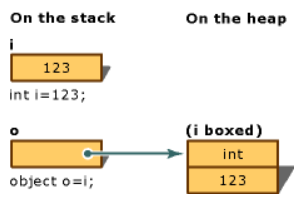
\includegraphics[width=0.4\linewidth]{images/boxing}
	\caption{Boxing}
	\label{fig:boxing}
\end{figure}



\subsection{Object}
\begin{itemize}
	\item \lstinline|object| ist ein Alias für \lstinline|System.Object|. Es ist die Basisklasse aller Typen.
\end{itemize}

\subsection{String}
\begin{itemize}
	\item \lstinline|string| ist ein Alias für \lstinline|System.String|
	\item String ist ein Reference Type
	\item Wie in Java ist ein String \textbf{nicht modifizierbar}, jedoch Verkettung mit + möglich
	\item Mit dem \lstinline|@| vor dem String Literal kann der String Sonderzeichen enthalten, die nicht escaped werden müssen.
\end{itemize}
\begin{lstlisting}
// Escape: The "File" can be \t found at \\server\share
@"The ""File"" can be \t found at \\server\share"

// Formatieren (konkatenieren)
string f = string.Format("A={0} and B={1}", a, b);

// Kopieren
string s2 = string.Copy(s1);

// Vergleichen
s1.Equals(s2) // Inhalt wird verglichen, nicht die Referenz
s1 == s2 // Inhalt wird verglichen, nicht die Referenz
s1.CompareTo(s2); // -1, 0, +1 
string.ReferenceEquals(s1, s2); // Achtung: String Pooling, nach Copy = False
\end{lstlisting}

\clearpage

\subsection{Arrays}
Einfachste Datenstruktur für Listen, bei welcher die Länge aller Dimensionen bei der Instanzierung bekannt ist. Wie in anderen Sprachen ist das Array zero-based(Index: [0 - (n-1)]), ein Referenztyp (zeigt auf Heap) und alle Werte nach Instanzierung initialisiert(false, 0, null, etc.).
\begin{lstlisting}
int[] array1 = new int[5]; // deklaration value type
int[] array2 = new int[] {1,2,3,4,5}; // deklaration & wertedefinition
int[] array3 = int[] {1,2,3,4,5,6}; // vereinfachte syntax ohne new
int[] array4 = {1,2,3,4,5,6}; // vereinfachte syntax ohne Typ / new
object[] array5 = new object[5]; // deklaration ref type
array1.Length // Get Length

// Blockmatritzen (Mehrdimensionale Arrays (rechteckig))  (Speichereffizienter, schnelleres Allozieren, schnellere Garbage Collection und vermeintlich schneller im Zugriff (Boundary Check wird nur bei 1-dimensionalen Array optimiert))
int[,] array1 = new int[3,2]; // Deklaration
int length = array1.Length; // Liefert 6
int length0 = array1.GetLength(0); // Liefert 3 (Laenge 0. Dimension)
int length1 = array1.GetLength(1); // Liefert 2 (Laenge 1. Dimension) 
int[,] multiDim2 = { {1,2,3} , {4,5,6} };  // Deklaration & Wertdefinition 

// Jagged Arrays (ausgefranst)
int[][] jaggedArray = new int[6][]; // Deklaration 
jaggedArray[0] = new int[4] { 1, 2, 3, 4 } // Wertdefinition 
\end{lstlisting}

\subsection{Indexer}
Ein Indexer erlaubt einfachen Zugriff auf ein Array. Er wird mit dem Keyword \lstinline|this| erstellt.
\begin{lstlisting}
class BookList {
	private string[,] books ={{},{},{}};

	public string this[int i1, int i2] {
		get { return books[i1, i2]; }
		set { books[i1, i2] = value;  } 
	}
}

// access
bookList[0, 0]
\end{lstlisting}

\subsection{List}
\begin{lstlisting}
var myList = new List<int>() { 1, 2, 3, 4, 5 }; // using System.Collections.Generic;
myList.Count(); // Or Property when var x = myList.Count;
myList.Add(6);
myList.Remove(4);
myList.Contains(6); // True
myList.ForEach(n => Console.WriteLine(n)); // 1,2,3,5,6
myList.Clear();
myList[4];
myList.IndexOf(4);
\end{lstlisting}

\pagebreak
\subsection{Namespaces}
Namespaces entspricht dem Package in Java und lässt den Code hierarchisch strukturieren. Ein Namespace ist nicht an die physische Struktur gebunden (in Java schon). Ein file kann mehrere Namespaces beinhaltet und ein Namespace kann in verschiedenen Files definiert sein. Er kann andere Namespaces, Klassen, Interfaces, Structs, Enums und Delegates enthalten.
\begin{lstlisting}
namespace A {
	using C;
	public class A : Base {
		C.externMethod();
	}
}
\end{lstlisting}

Neu, wenn nur ein Namespace in einer Datei folgende Schreibweise präferiert. Spart in jeder Zeile 4 Zeichen (File-scoped Namespace). Nur ein Namespace pro File ist so dann erlaubt:
\begin{lstlisting}
namespace A;
//.... Code ....
\end{lstlisting}

Namespace können auch mittels Alias-Namen geladen werden:
\begin{lstlisting}
using F = System.Windows.Forms;
//.... Code ....
F.Button b;
\end{lstlisting}

Weiter gibt es auch globale Imports (Meist Datei GlobalUsings.cs). Dies geht auch implizit via *csproj-Datei. Nicht jede SDK supported diese Funktion:
\begin{lstlisting}
using static Azure.Core;
\end{lstlisting}

\subsection{Main Methode}
Die Main Methode ist die Einstiegspunkt in die Anwendung. Sie ist zwingend für Executables (Console Application, Windows Application, etc.). Darf genau einmal Vorkommen. Wenn es mehrere gibt, muss mann in der csproj-Datei explizit angeben, welche verwendet werden soll. Sie befindet sich meist in der Datei Program.cs. Sie muss folgende Signatur haben:
\begin{lstlisting}
// Expamles
static void Main() { }
static int Main() { }
static void Main(string[] args) { }
static int Main(string[] args) { }
static async Task Main() { }
static async Task<int> Main() { }
static async Task Main(string[] args) { }
static async Task<int> Main(string[] args) { }
\end{lstlisting}

Auf Arbumente kann unterschiedlich zugegriffen werden. Per Default greift man über ein string[]-Parameter zu. Ohne diesen Parameter ist es auch möglich über die statische Methode \lstinline|System.Environment.GetCommandLineArgs();| darauf zuzugreifen. Neu kann auch die Main-Methode als entry-Point weggelassen werden dank Top-level Statements. Die Regeln sind folgende:
\begin{itemize}
	\item Nur 1x pro Assembly erlaubt
	\item Argumente heissen fix \lstinline|args|
	\item Exit Codes elaubt: \lstinline|return someIntValue;|
	\item VOR dem top-level Statements können usings definiert werden
	\item NACH dem top-level Statements können Typen definiert werden
\end{itemize}

\section{Variablen und Properties}
\subsection{Konstanten}
Der Wert einer Konstante muss zur Compilezeit verfügbar sein.
\begin{lstlisting}
const long size = int.MaxValue;
\end{lstlisting}

\subsection{ReadOnly}
Readonly Felder müssen in der Deklaration oder im Konstruktor initialisert werden. Readonly Variablen sind äquivalent mit Java final Felder
\begin{lstlisting}
	readonly DateTime date1 = DateTime.Now;
	
	class Test {
		private readonly int myProp;
		public int MyProp {
			get { return myProp; }
		}
		
		public Test() {
			myProp = 42;
		}
	}
\end{lstlisting}

\subsection{Properties}
Eine Property ist ein Wrapper um Getter und Setter. Get und Set können einzeln weggelassen werden. (read-only, write-only) Bei Set besteht zudem die Möglichkeit das Flag private zu setzen.
\begin{lstlisting}
	// Backing Field
	private int lenght;
	
	public int Length {
		get { return length; }
		// private is optional
		private set { length = value; } 
	}
	
	MyClass mc = new MyClass();
	mc.Length = 12;
	int length= mc.Length;
	
\end{lstlisting}

\subsubsection{Auto Properties}
Bei Auto Properties wird das Backing Field sowie die zugehörigen Getter und Setter automatisch generiert.
\begin{lstlisting}
	// Auto Property: Backing field is auto generated
	public int LengthAuto { get; set; }
	public int LengthInitializes {get; /* set; */ } = 5;
\end{lstlisting}

\subsubsection{Properties direkt initialisieren}
Properties können bei der Objekt erstellung direkt initialisiert werden.
\begin{lstlisting}
class MyClass
{
    private int length; // Backing-Field
    
    // Property
    public int Length 
    {
        get {return length; }
        set { length = value; } 
    }
    public int Width { get; set; } 
} 

	MyClass mc = new MyClass() {
		Length = 1;
		Width = 2;
	}
\end{lstlisting}

\subsubsection{Abstrakte Properties/Indexes}
Abstrakte Properties/Indexes haben kein Anweisungsteil. Get und Set werden analog der Auto Properties mit einem Semikolon abgeschlossen. Wichtig ist das bei der Implementation Get und Set Kombination identisch sein muss.

\section{Methoden}
Im C\# hat man zwei verschiedene Ausprägungen von Methoden:
\begin{itemize}
	\item Prozedur/Aktion: ohne Rückgabewert
	\item Funktion: mit Rückgabewert
\end{itemize}
\subsection{Overloading}
Methoden können \textbf{überladen} werden. (Unterschiedliche Anzahl Parameter, Unterschiedliche Typen, Unterschiedliche Parametertypen (ref/out) aber immer gleicher Name). Rückgabewert ist \textbf{kein} Unterscheidungsmerkmal.
\begin{lstlisting}
public static void Foo(int x);
public static void Foo(doubly y);
public static void Foo(int x, int y);
public static void Foo(params int[] x); // params array = normales array

// sollte man nicht machen. Design Problem!
public static void Foo(int ref x);
public static void Foo(int out x);
\end{lstlisting}

\subsection{Call by value}
Es wird eine Kopie des Stack Inhalts übergeben
\begin{lstlisting}
void IncVal(int x){x = x + 1;}
int val = 3; 
IncVal(val); // val = 3;
\end{lstlisting}

\subsection{Call by reference}
Adresse der Variable wird übergeben. Mit dem \lstinline|ref| Keyword können auch Werttypen als Referenz übergeben werden. Wichtig die Variable muss zuerst initialsiert werden.
\begin{lstlisting}
void IncRef(ref int x) {x++; }
int value=3; //value must be initialized first
IncRef(ref value); // pass reference, value = 4;
\end{lstlisting}

\subsection{Out Parameter}
Das \lstinline|out| Keyword erlaubt es Werte by Reference zu übergeben. Es funktioniert wie das \lstinline|ref| Keyword, mit dem Unterschied, dass die Variable nicht im Vorhinein initialsiert werden muss. Es ist ebenfalls möglich, die Variable mit dem \lstinline|out| direkt beim Methodenaufruf zu deklarieren.
Das \lstinline|out| Keyword muss beim Aufrufer und bei der Methode deklariert werden.
\begin{lstlisting}
static void Init(out int a) {
	a = 10;
}
// usage
int value1 
Init(out value1) //value1 = 10;
// declaration in method call
Init(out int value2); // value2 is now 10 
\end{lstlisting}

\subsection{Params Array}
Erlaubt beliebig viele Parameter. Das params Array muss am Ende der Deklaration stehen.
\begin{lstlisting}
void Sum(out int sum, params int[] values) { .. }
Sum(out sum2, 1,2,3,4);
\end{lstlisting}

\subsection{Optionale Parameter (Default Values)}
Erlaubt ermöglicht Zuweisung eines Default Values. Die Optionalen Parameter dürfen erst am Schluss deklariert werden. Default Werte können bei \lstinline|out| und \lstinline|ref| Parameter nicht verwendet werden.
\begin{lstlisting}
private void Sort(
	int[] array,            // Erforderlich
	int from = 0,           // Optional
	int to = -1,            // Optional
	bool ascending = true,  // Optional
	bool ignoreCase = false // Optional
	){ .. }
\end{lstlisting}

\subsection{Named Parameter}
Optionale Parameter können über den Namen identifiziert und übergeben werden.
\begin{lstlisting}
Sort(a, ignoreCase: true, from: 3);
\end{lstlisting}

\subsection{Virtual}
Bei C\# wird alles statisch gebunden. Mit dem Keyword \lstinline|virtual|, wird dynamisch gebunden. Bei einer virtuellen Methode wird deshalb die überschriebene Methode in der Subklasse aufgerufen. Virtual kann nicht mit folgenden Keywords verwendet werden.
\begin{itemize}
	\item \lstinline|static|
	\item \lstinline|abstract| (implizit virtual)
	\item \lstinline|override| (implizit virtual)
\end{itemize}

\subsection{Override}
Mit dem Keyword \lstinline|override| können \lstinline|virtual| Methoden überschrieben werden. Die Signatur muss dabei identisch sein. Man spricht von dynamischem Binding.


\begin{lstlisting}
public class Base {
	public virtual void Invoke() {
		Console.WriteLine("Base");
	}
}
public class Derived : Base {
	public override void Invoke() {
		Console.WriteLine("Derived");
	}
}

Base a = new Base();
Base b = new Derived();
Derived c = new Derived();

a.Invoke(); // base
b.Invoke(); // derived
c.Invoke(); // derived
\end{lstlisting}

\subsection{Methoden überdecken mit New}
Mit \lstinline|new| weiss der Compiler, dass der Member bewusst überdeckt wurde. Man spricht von \textbf{statischem Binding}. Es wird immer die Methode des statischen Typs ausgeführt. New kann \textbf{nicht} mit \lstinline|override| verwendet werden, jedoch mit \lstinline|virtual|.
\begin{lstlisting} 
public class Base {
	public void Invoke() {
		Console.WriteLine("Base");
	}
}
public class Derived : Base {
	public new void Invoke() {
		Console.WriteLine("Derived");
	}
}

Base a = new Base();
Base b = new Derived();
Derived c = new Derived();

a.Invoke(); // base
b.Invoke(); // base
c.Invoke(); // derived
\end{lstlisting}

\subsection{Dynamic Binding}
Man spricht von Dynamic Binding, wenn die Methoden des dynamischen Typs aufgerufen werden. Dazu gibt es ein vereinfachtes Regelwerk:
\begin{itemize}
	\item Falls der dynamische Typ konkreter als der statische Typ und die Methode \lstinline|virtual| ist.
	\item Suche Vererbungs-Hierarchie von oben nach unten nach konkrester Methode mit Schlüsselwort \lstinline|override|
\end{itemize}

\subsection{Abstrakte Methoden}
Abstrakte Methoden haben statt dem Anweisungteil ein Semikolon und sind implizit \lstinline|virtual|, dürfen jedoch \textbf{nicht} \lstinline|static| oder \lstinline|virtual| sein.
\begin{lstlisting}
abstract class Sequence { public abstract void Add(object x); }
\end{lstlisting}

\subsection{Sealed}
Mit \lstinline|sealed| weiss der Compiler, dass die Methode (kein Overriding) oder Klasse (keine Vererbung) nicht mehr verändert wird.
Bei der Methode muss es in Kombination mit \lstinline|override| verwendet werden.
Das Überdecken von versiegelten Members mit \lstinline|new| ist erlaubt
Es ist das Pendant zum Java \lstinline|final|.
\begin{lstlisting} 
public override sealed void MyFunc(); //works
public sealed void MyFunc2(); // Compiler-Error
\end{lstlisting}

\section{Klassen, Structs}
\subsection{Klassen}
\begin{itemize}
	\item Klassen sind Refenztypen die auf dem Heap abgelegt werden
	\item Klassen können ineinander verschachtelt sein. Die Inner Class hat dabei Zugriff auf alle Member der Outer Class. Die Inner Class wird mit \lstinline|OuterClass.InnerClass inner = new OuterClass.InnerClass();| initialisiert.
	\item Klassen können statisch sein. Statische Klassen können nicht abgeleitet werden. Es gibt auch statische Imports \lstinline|using static System.Math|
	\item Hat immer einen Default Konstruktor, sofern nicht ein anderer definiert wurde.
	\item Links steht immer der statische Typ und rechts der dynamische
\end{itemize}

\subsubsection{Type Casts}
Type Casts können mit den runden Klammern oder mit dem Keyword \lstinline|as| gemacht werden. \lstinline|as| liefert \lstinline|null| zurück, wenn nicht gecasted werden kann (anstatt eine Exception zu werfen).
\begin{lstlisting}
// type cast
Base b = new Sub();
Sub s = (Sub) b; // could throw InvalidCastException

// cast with 'as'
Sub s = b as Sub; // returns null if cast not possible

\end{lstlisting}

\subsubsection{Typprüfung}
Die Typprüfung gibt \lstinline|true| wenn:
\begin{itemize}
	\item Typ von "obj" identisch wie "T" ist (exakt gleicher Typ)
	\item Typ von "obj" eine Sub-Klasse von "T" ist
\end{itemize}
\begin{lstlisting}
class Base {}
class Sub: Base {}
class SubSub: Sub {}
public static void Test() {
  SubSub a = new SubSub();
  if (a is SubSub) {   /* True */ }
  if (a is Sub) { /* True */ } 
  if (a is Base) { /* True */ }
  a = null; 
  if (a is SubSub) { /* // False / NULL /* } 
} 
\end{lstlisting}
\subsubsection{Typprüfungen mit implizitem Type Cast}
Ebenfalls ist es möglich ein dynamischen Typ zu prüfen und direkt zu casten.
\begin{lstlisting}
public class Animal { public string Sound { get; } = "Sound like an Animal"; }
public class Dog : Animal { public new string Sound { get; } = "Barking like a Dog"; }

Animal animalJoe = new Dog();
            Console.WriteLine(animalJoe.Sound); // "Sounds like an Animal"
            if (animalJoe is Dog dogJoe) {
                Console.WriteLine(dogJoe.Sound);// "Barking like a Dog"
            }
\end{lstlisting}


\subsubsection{Operatoren Überladen}
\begin{lstlisting}
public class Vector{
	private int x, y;
	
	public Vector(int x, int y) {};
	
	// must be static
	public static Vector operator + (Vector a, Vector b) {
		return new Vector(a.x + b.x, a.y + b.y);
	}						
}
\end{lstlisting}


\subsubsection{Partial Class}
Das \lstinline|partial| Keyword erlaubt die Definition in mehreren Files. Es sind auch partielle Methoden möglich
\begin{lstlisting}
partial class MyClass { public void Test1() { .. } }
partial class MyClass { public void Test2() { .. } }

MyClass mc = new MyClass();
\end{lstlisting}

\subsection{Abstrakte Klassen}
\begin{itemize}
	\item Abstrakte Klassen können nicht direkt instanziert werden.
	\item Alle abstrakte Member müssen implementiert sein (\lstinline|override|)
\end{itemize}
\begin{lstlisting}
abstract class Sequence {
	public abstract void Add(object x); // implicit virtual, no implementation
	public abstract string Name { get; }; // property
	public abstract object this[int i]{ get; set; }; // indexer
	public abstract event EventHandler OnAdd; // Event;
	
	public override string ToString() {return Name; }; 
}

class List : Sequence {
	public override void Add(object x)
}
\end{lstlisting}

\subsection{Sealed Klassen}
Von versiegelten ''\lstinline|sealed|'' Klassen kann nicht abgeleitet werden. Es verhält sich also wie das \lstinline|final| bei Java.
\begin{lstlisting}
sealed class Sequence {
	// members can also be sealed:
	public sealed void X();
}

class List : Sequence {} // Compiler error

class Sequence {
	// cannot be overwritten, but 'new' is possible
	public sealed void X();
}

\end{lstlisting}

\subsection{Statische Klassen}
Statische Klassen sind implizit \lstinline|sealed|. Sie dürfen nur statische Member enthalten und können nicht instanziiert werden.
\begin{lstlisting}
static class MyMath {
	public const double Pi = 3.14159;
	public static double Sin(Double x) { .. }
}
\end{lstlisting}
\clearpage

\subsection{Structs}
\begin{itemize}
	\item Structs sind Valuetypen die auf Stack liegen
	\item Structs sind Valuetype und können deshalb nie \lstinline[]|null| sein.
	\item Structs können weder vererben noch erben. (Interfaces sind aber möglich)
	\item Structs benötigen weniger Speicherplatz wie Klassen
	\item Es gibt keinen parameterlosen Konstruktor!
	\item Struct Felder dürfen nicht initialisiert werden
	\item Stucts sollten in folgenden Fällen verwendet werden
	      \begin{itemize}
		      \item Repräsentiert einen einzelnen Wert
		      \item Instanzgrösse ist kleiner als 16 Byte (128 Bit)
		      \item Ist "immutable" (nicht der default)
		      \item Wird nicht häufig geboxt
		      \item Ist entweder kurzlebig oder wird meist in andere Objekte eingebettet
	      \end{itemize}
\end{itemize}
\begin{lstlisting}
 public struct FinalPoint
{
    public readonly int x;
    public readonly int y; 
    public FinalPoint(int x, int y) //Konstruktor nur mit Parameter
    {
        this.x = x;
        this.y = y;
    }
}
//Verwendung
FinalPoint FinalPoint1 = new FinalPoint(1,2);
\end{lstlisting}

\subsection{Konstruktoren}
Es gibt verschiende Konstruktoren:
\begin{description}
	\item[statische Konstruktoren] Ist nicht von aussen verfügbar und wird für Initialisierungsarbeiten verwendet werden. Er wird nur für die erste Instanz aufgerufen. Dieser Konstruktor ist zwingend parameterlos und die Sichtbarkeit darf nicht angegeben werden. (keyword: \textit{static})
	\item[nicht statische Konstruktoren] Der normale Konstruktor
	\item[private Konstruktoren] Können nur intern verwendet werden. Gibt es einen privaten Konstruktor, so wird \textbf{kein} Default Konstruktor erzeugt.
\end{description}
\begin{lstlisting}
public class MyClass {
	// call super constructor
	public MyClass(int a) : base(a) {}

	// call constructor in same class
	public MyClass(int a) : this(a, false) {}
	
	public MyClass(int a, boolean b) {}
	
	// static constructor
	static MyClass() {}
}
\end{lstlisting}

\subsection{Initialisierungsreihenfolge}
\begin{enumerate}
	\item Statische Felder (Unterklasse zuerst) (nur 1x pro Klasse, falls mehrere Instanzen erzeugt werden!)
	\item Statische Konstruktoren (Unterklasse zuerst) (nur 1x pro Klasse, falls mehrere Instanzen erzeugt werden!)
	\item Felder (Unterklasse zuerst, in Deklarationsreihenfolge)
	\item Konstruktoren (Oberklasse zuerst)
\end{enumerate}



\begin{minipage}[t]{1\textwidth}
	\centering
	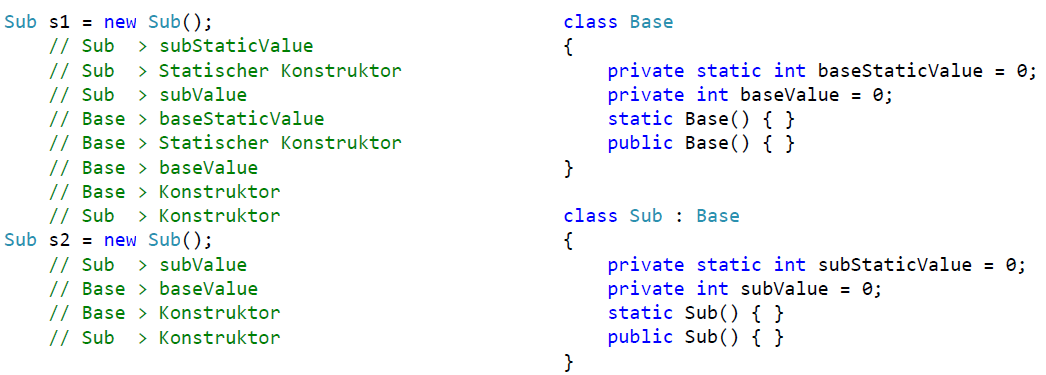
\includegraphics[width=0.9\linewidth]{images/init_order}
	\captionof{figure}(Initialisierungs-Reihenfolge (mit Vererbung))
\end{minipage}

\begin{minipage}[t]{1\textwidth}
	\centering
	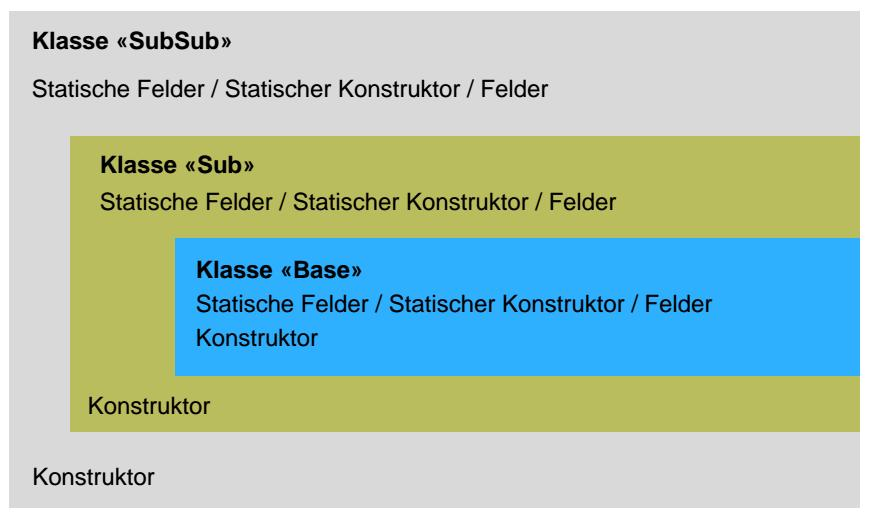
\includegraphics[width=0.9\linewidth]{images/initialisierungsreihenfolge}
	\captionof{figure}(Initialisierungsreihenfolge)

\end{minipage}

\begin{minipage}[t]{1\textwidth}
	\centering
	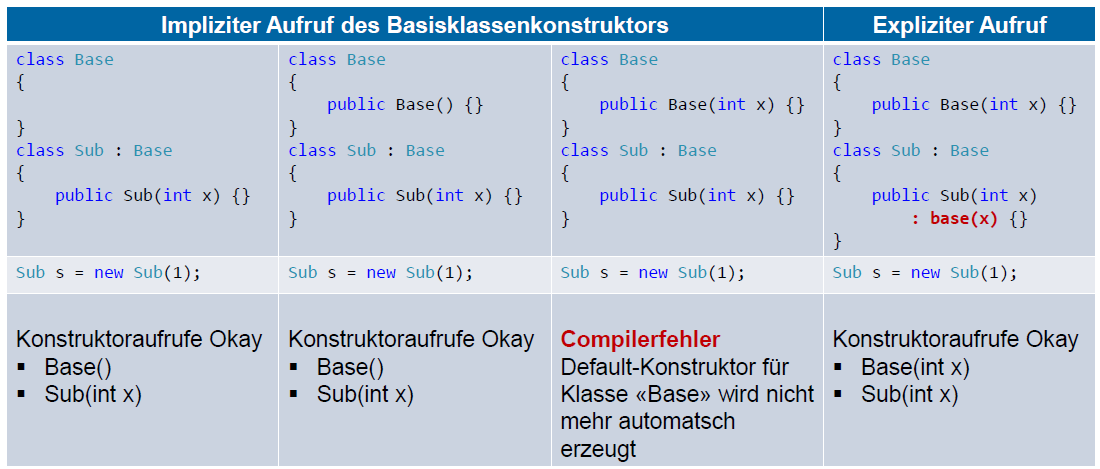
\includegraphics[width=\linewidth]{images/init_constructors}
	\captionof{figure}(Konstruktoraufrufe)
\end{minipage}

\subsection{Destruktoren}
Der Destruktor ruft im Hintergrund die Methode Finalize auf.
\begin{lstlisting}
class MyClass {
	~MyClass() {}
}
\end{lstlisting}

\subsection{Operator Overloading}
Die Methode muss \lstinline|static| sein und das Keyword \lstinline|operator| verwenden. \textbf{Mindestens 1 Parameter} muss vom Typ der enthaltenen Klasse sein!
\begin{lstlisting}
class MyClass {
	public static MyClass operator + (MyClass a, MyClass b) {
		return new MyClass(a.x + b.x, a.y + b.y);
	}
	public static MyClass operator ~(MyClass a) {
		return new MyClass();
	}
	
	public static MyClass operator + (int a, int b) {..}// does not work!
}

// usage
MyClass mc3 = mc1 + mc2;
\end{lstlisting}

Folgende Operatoren können überladen werden
\begin{figure}[!ht]
	\centering
	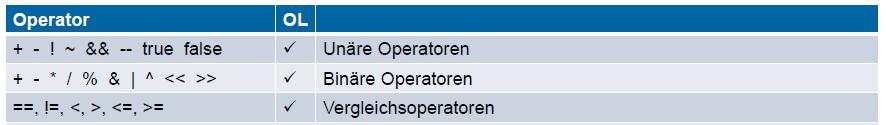
\includegraphics[width=0.7\linewidth]{images/operator_overloading}
	\caption{Operatoren Überladen}
	\label{fig:operatoroverloading}
\end{figure}


\section{Interfaces}
\begin{itemize}
	\item Kann \textbf{nicht} direkt instanziert werden
	\item Bei Membern von einem Interface wird keine Sichtbarkeit angegeben
	\item Name beginnt mit grossem I
	\item Member sind implizit \lstinline[language=C]|abstract virtual|
	\item Member dürfen nicht \lstinline|static| oder ausprogrammiert sein
	\item In der Klasse, welche Interface implementiert, müssen alle Interface-Member vorhanden sein.
	\item \lstinline|override| ist nicht nötig
	\item Seit C\# 8.0 können Interfaces auch Default-Implementationen haben und so dennoch programmiert werden.
\end{itemize}
\begin{lstlisting}
	interface ISequence {
		void Add(object x);
		string Name { get; }
		object this[int i] { get; set; }
		event EventHandler OnAdd;
	}
	
class List : Base, ISequence, I2 {
	public void Add(object x) { /* ... */ }
	public string Name { get { /* ... */ } }
    public object this[int i] { get { /* ... */ } set { /* ... */ } }
    public event EventHandler OnAdd;
} 
\end{lstlisting}

\subsection{Interface Naming Clashes}
Es ist möglich, das zwei implementierte Interfaces dieselben Methoden haben. Dann ist es möglich die Member-Methoden und/oder ein Default-Verhalten zu implementieren.

\begin{lstlisting}
class ShoppingCart : ISequence, IShoppingCart {
    public void Add(object x) { /* ... */ } 
    void ISequence.Add(object x) { /* ... */ } 
    int IShoppingCart.Add(object x) { /* ... */ } // also possible if same return value 
}
\end{lstlisting}

\section{Enum}
Eine Enumeration ist eine vordefinierte Liste von Konstanten mit einem optionalen Wert. Enum leitet von Int32 ab. Um Speicherplatz zu sparen, könnte man auch von byte, sbyte, short etc erben(Sollte nicht gemacht werden).
\begin{lstlisting}
enum Days { Sunday = 42, Monday, Tuesday, Wednesday, Thursday, Friday, Saturday };
Days today = Days.Monday;
if (today == Days.Monday) { /* ... */ }

// Two ways to parse Enum out of a String
Enum.Parse(typeof(Days), "Monday");
MyEnum myEnum;
Enum.TryParse("Monday", out myMonday); // returns true if successful

// Print all Enum Types
foreach(string name in Enum.GetNames(typeof(Days))) {
	Console.WriteLine(name);
}
\end{lstlisting}
Enums sind mit Werten definiert. Standardmässig beginnt es mit 0. Jedoch kann das auch angepasst werden.

\begin{lstlisting}
enum Days { Sunday, Monday, Tuesday, Wednesday, Thursday, Friday, Saturday };
int sundayValue = (int)Days.Sunday; Console.WriteLine("{0} / #{1}.", Days.Sunday, sundayValue); // Ausgabe: Sunday / #0
int fridayValue = (int)Days.Friday; Console.WriteLine("{0} / #{1}.", Days.Friday, fridayValue); // Ausgabe: Friday / #5 

//oder mit eigener Wertedefinition:
enum DaysWithValues { Sunday = 10, Monday, Tuesday, Wednesday, Thursday, Friday = 9, Saturday }; 

int sundayValue = (int)DaysWithValues.Sunday; Console.WriteLine("{0} / #{1}.", DaysWithValues.Sunday, sundayValue); // Ausgabe: Sunday / #10
int fridayValue = (int)DaysWithValues.Friday; Console.WriteLine("{0} / #{1}.", DaysWithValues.Friday, fridayValue); // Ausgabe: Friday / #9 
\end{lstlisting}


\section{Generics}
Generics erlaub die Implementationen von generischen Strukturen ohne die Verwendung von \lstinline|object|. Anstelle von \lstinline|object| wird \lstinline|T| verwendet.
Generics können in Klassen/Structs, Interfaces, Delegates/Events und Methoden verwendet werden. Während der Verwendung einer der möglichen Strukturen wird \lstinline|T| beispielsweise als \lstinline|string| deklariert.  Generics sind für Value Types schneller (kein Boxing nötig), bei Reference Type jedoch nicht. (Verglichen mit \lstinline|object|)
\begin{lstlisting}
public class Buffer<T> {
	T[] items;
	public void Put(T item) { /* ... */ }
	public T Get() { /* ... */ }
}

//mehrere Typparameter

public class Buffer<TElement, TPriority> {
    TElement[] items; 
    TPriority[] priorities; 
    public void Put( TElement item, TPriority prio) { /* ... */ } 
} 
\end{lstlisting}

\subsection{Type Constraints}
Mit dem Keyword \lstinline|where| kann eine Regel definiert werden, die der dynamische Typ erfüllen muss.

\begin{description}
	\item[Kovarianz] Erlaubt die Zuweisung von stärker abgeleiteten Typen als urprüfunglich angegeben
		\begin{lstlisting}
public interface IBuffer<in T>
\end{lstlisting}
	\item[Kontravarianz] Erlaubt die Zuweisung von weniger stark abgeleiteten Typen als ursprünglich angegeben.
		\begin{lstlisting}
public interface IBuffer<out T>
\end{lstlisting}
\end{description}

\begin{table}[ht]
	\centering
	\begin{tabu} to \linewidth {l X}
		\toprule
		Constraint                & Beschreibung                                                                                           \\
		\midrule
		where T : struct          & T muss ein Value Type sein.                                                                            \\
		where T : class           & T muss ein Reference Type sein. Darunter fallen auch Klassen, Interfaces, Delegates                    \\
		where T : new()           & T muss einen \textbf{parameterlosen} "public" Konstruktor haben. Wird benötigt um new T() zu erstellen
		Dieser Constraint muss – wenn mit anderen kombiniert – \textbf{immer zuletzt
		aufgeführt} werden                                                                                                                 \\
		where T : "ClassName"     & T muss von Klasse "ClassName" ableiten.                                                                \\
		where T : "InterfaceName" & T muss Interface "InterfaceName" implementieren.                                                       \\
		where T : TOther          & T muss identisch sein mit TOther.
		oder
		T muss von TOther ableiten.                                                                                                        \\
		where T : class?          & T muss eine Nullable Reference Type sein.
		Darunter fallen auch Klassen, Interfaces, Delegates. (Mehr im nächsten Kapitel)                                                    \\
		where T : not null        & T musse in Non-Nullable Value Type oder Reference Type sein.                                           \\
		\bottomrule
	\end{tabu}
	\caption{Type Constraints}
\end{table}
\subsubsection{Beispiele}
\begin{lstlisting}
class MyClass<T, P> where T : IComparable { .. }
public T GetInstance<T>() where T : new() {
	return new T(); // must have default constructor
}
\end{lstlisting}

\begin{lstlisting}
public void FillList<T>(T source) where T : List<int>, IEnumerable<int>  { source.Add(1); source.Add(2); source.Add(3); }
\end{lstlisting}


\begin{lstlisting}
class ExamplesCombiningConstraints<T1, T2>
where T1 : struct 
where T2 : Buffer, IEnumerable<T1>, new()
{ /* ... */ } 
\end{lstlisting}

\subsection{Typprüfungen}
\begin{lstlisting}
Type t = typeof(Buffer<int>); // t.Name = Buffer[System.Int32]
\end{lstlisting}

\subsection{Generische Vererbung}
Generische Klassen können von anderen generischen Klassen erben:
\begin{description}
	\item[Normale Klassen] \lstinline|class MyList<T> : List { } |
	\item[Weitergabe des Typparameters an Basisklasse] \lstinline|class MyList<T> : List<T> { } |
	\item [Konkretisierte generische Basisklasse] \lstinline|class MyIntList : List<int> { } |
	\item[Mischform] \lstinline|class MyIntKeyDict<T> : Dictionary<int, T> { } |
\end{description}
\begin{lstlisting}
// Zuweisung mit "normaler" Basisklasse
class MyList<T> : MyList { /* ... */ } 
class MyDict<TKey, TValue> : MyList { /* ... */ } 
public void Test() {
    MyList l1 = new MyList<int>();
    MyList l2 = new MyDict<int, float>();
    object o1 = new MyList<int>();
    object o2 = new MyDict<int, float>(); 
} 

// Zuweisung mit generischer Basisklasse
class MyList2<T> : MyList<T> { } 
class MyDict<TKey, TValue> : MyList<TKey> { }
public void Test() { 
    MyList<int> l1 = new MyList2<int>();
    MyList<int> l2 = new MyDict<int, float>();
    MyList<int> l3 = new MyList<float>(); //Compilerfehler: Typparameter inkompatibel
    MyList<object> l4 = new MyList<float>(); //Compilerfehler: Typparameter inkompatibel
}
\end{lstlisting}
\subsection{Generische Delegates}
Es ist auch möglich Delegates generisch zu machen. Hier einige Beispiele:
\begin{lstlisting}
public delegate void Action<T>(T i); 
public delegate void Action<T1,T2>(T1 obj1, T2 obj2); 
public delegate TResult Func<T>(T arg); 
public delegate bool Predicate<T>(T obj); 
\end{lstlisting}

\subsection{Generische Collections}
Es gibt eine Liste von generischen Collections, hier einige davon:

\begin{itemize}
	\item \lstinline| List<T> |
	\item \lstinline| SortedList<TKey, TValue> |
	\item \lstinline| Dictionary<TKey, TValue> |
	\item \lstinline| SortedDictionary<TKey, TValue> |
	\item \lstinline| LinkedList<T> |
	\item \lstinline| Stack<T>|
	\item \lstinline| Queue<T>|
\end{itemize}

\section{Nullability}
Tony Hoare nennt das Einführen der Null Reference als "Bilion-Dollar-Mistake".

\subsection{Default operator \/ literal}
\lstinline|default(T) / default| liefert den Default-Wert für angegebene Typen. Bei Reference Types ist die \lstinline|null|. Bei Value Types ist dies entweder \lstinline|0|, \lstinline|false| oder \lstinline|\0|. Bei Vergleiche ()\lstinline|x is null|) gibt es folgendes Verhalten:
\begin{description}
	\item[Reference Types] \lstinline|true| wenn \lstinline|x| \lstinline|null| ist, ansonsten \lstinline|false|
	\item[Value Types] \lstinline|false| in jedem Fall. Compilerfehler wenn \lstinline|T : struct|
\end{description}
\begin{lstlisting}
public void NullExamples<T>()
{
	// Nullwerte zuweisen
	T x1 = null; // Compilerfehler
	T x2 = 0; // Compilerfehler
	T x3 = default(T); // OK
	T x4 = default; // OK (C# 7.1)

	// Nullwerte prüfen
	if (x1 is null)
	{
	/* ... */
	}
}
\end{lstlisting}

\subsection{Structs / Value Types}
Null-Zustand exisitert nicht und muss quasi erzwungen werden (Seit 2002 /.NET 2.0 C\# 2).

\subsubsection{Struct <Nullable>}
Value Types kann nun dank Generics "null" zugewiesen werden. Dazu dient die Klasse \lstinline|System.Nullable<T>|.
\begin{table}[ht]
	\centering
	\begin{tabular}{lll}
		\textbf{Status} & \textbf{HasValue} & \textbf{Value} \\
		null            & false             & ?              \\
		not null        & true              & 123
	\end{tabular}
	\caption{Werte je nach Status}
\end{table}

Wenn auf Value zugegriffen wird und \lstinline|HasValue| \lstinline|false| ist, wird eine \lstinline|System.InvalidOperationException| geworfen.

\begin{lstlisting}
public struct Nullable<T>
where T : struct
{
	public Nullable(T value);

	public bool HasValue { get; }
	public T Value { get; }
}
\end{lstlisting}

\subsubsection{T? Syntax}
Die \lstinline|T?| Syntax dient zur verbesserung der Lesbarkeit. So kann \lstinline|null| direkt zugewiesen werden.
\begin{lstlisting}
int? x = 123;
int? y = null;
\end{lstlisting}

\subsubsection{Sicheres Lesen \& Type Casts}
\begin{lstlisting}
int? x = null;

// Klassisch
int x1 = x.HasValue
	? x.Value
	: default;

// Via Methode
int x2 = x.GetValueOrDefault();

// Via Methode inkl. eigenem Default
int x3 = x.GetValueOrDefault(-1);
\end{lstlisting}

\subsection{Klassen / Reference Types}
Null-Zustand ist in Runtime abgebildet. Zugriff auf Null References führt zu \lstinline|NullReferenceException|. Dies ist nicht mehr eliminierbar. Doch Compiler bietet seit C\# 8 vermeidung von Zugriff auf Null Referenzen an. (Seit 2019 / .NET Core 3.0 / C\# 8)
Compiler generiert Warnungen basierend auf "static flow analysis".
\newline\newline
Hinweis: Implementation unterscheidet sich massiv von "Nullable Value Types"
\subsubsection{Syntax}
Die Compiler Warnungen können im .csproj aktiviert werden innerhalb der \lstinline|<PropertyGroup>| mittels \lstinline|<Nullable>enable</Nullable>| und deaktiviert mittels \lstinline|<Nullable>disable</Nullable>|. Die Warnungen können auch im Code via Präprozessor Direktiven mittels \lstinline|#nullable enable| aktiviert und mit \lstinline|#nullable disable|  deaktiviert werden.
\newline\newline
Eine Variable kann mittels \lstinline|?| als "nullable" deklariert werden. Weiter gibt es den Null-forgiving Operator \lstinline|!|, welcher den Compiler verspricht, dass die Variable nicht \lstinline|null| ist. Dies ist sehr gefährlich und sollte nur mit bedacht eingesetzt werden, da Compile Time != Runtime (inkonsistent).
\begin{lstlisting}
string? nameNull = null;
string name = nameNull; // Warning

if (nameNull is null) // or "name == null"
{
	name = nameNull; // Warning
	name = nameNull!; // OK, but wrong
}
else
{
	name = nameNull; // OK
}
\end{lstlisting}

\subsection{Syntatic sugar}
\subsubsection{is null \/ is not null (Pattern matching)}
\begin{description}
	\item[Value Types] Verwendet \lstinline|System.Nullable<T>.HasValue|
	\item[Reference Types] Prüft ob es sich um eine Null Referenz handelt mittels \lstinline|object.ReferenceEquals()|
\end{description}

Der \lstinline|==| Operator sollte nicht verwendet werden, da er manuell überschrieben worden sein könnte.
\begin{lstlisting}
int? x = null;
string s = null;

bool b1a = x is null; // true
bool b1b = x is not null; // false
	
bool b2a = s is null; // true
bool b2b = s is not null; // false
\end{lstlisting}

\subsubsection{?? (Null-Coalescing Operator)}
Binäre Operator. Gibt den Linken Teil zurück, sofern nicht null. Ansonsten wird der Rechte Teil zurückgegeben.
\begin{lstlisting}
int? x = null;
int i = x ?? -1; \\ -1

\\ Auch möglich
int i = x ?? throw new ArgumentNullException(nameof(x));
\end{lstlisting}
\subsubsection{??= (Null-Coalescing Assignment)}
Setzt die Variable (linker Teil) auf einen gewünschten wert, sofern diese Variable null ist. Keine Operation wenn die Variable ungleich null ist.
\begin{lstlisting}
int? x = null;
int i ??= -1; \\ x hat nun Wert "-1"

int? x = 10;
int i ??= -1; \\ x hat immernoch Wert "10"
\end{lstlisting}

\subsubsection{?. (Null-Conditional Operator)}
Führt den rechten Teil aus, sofern der linke Teil nicht null ist. Andernfalls wird null geliefert. (Sofern Methode nicht void liefert). Funktioniert auch mit Delegates über \lstinline|.Invoke()|.
\begin{lstlisting}
object o = null;
Action a = null;

string s = o?.ToString(); // null
a?.Invoke();
\end{lstlisting}

\section{Record Types}
Record Types sind ein reines Compiler Feature und dienen zum erstellen von Datenrepräsentations-Klassen und Reduktion von Boilerplate Code.


\begin{description}

	\item[Vereinfacht] Arbeit mit Nullable Reference Types.
	\item[Grundidee] Record Types sollten immutable sein.
\end{description}
\begin{lstlisting}
	public record [class|struct] Person(int Id, string Name);
\end{lstlisting}

Folgender Code wird generiert:
\begin{itemize}
	\item Konstruktor
	\item Properties (Immutable)
	\item Value equality
	\item Darstellung (ToStringMethode, etc.)
	\item Vererbung wird berücksichtigt (z.B. Equality)

\end{itemize}
\subsection{Deklarationsmöglichkeiten}
Eine manuelle Deklaration wie normale Klassen ist möglich. So werden teilweise To-String und Value Equality generiert. Besser ist: Positional Syntax verwenden (Siehe oben)
\begin{lstlisting}
public record Person
{
    public Person() : this(0, "") { }
    public Person(int id, string name)
    {
        Id = id;
        Name = name;
	}

    public int Id { get; init; }
    public string Name { get; init; }
}

// Anwendungsbeispiel
Person p1 = new();
Person p2 = new(1, "Mary");
\end{lstlisting}

Man kann auch eine gemischte Variante nutzen. Um so eigene Methoden zu erweitern. Wichtig: Generierte Properties werden als Init-Only setter generiert. Man kann so eine Warnung herausgeben, wenn Name leer.
\begin{lstlisting}
public record Person(int Id)
{
    public string Name { get; init; }
    public void DoSomething() { }
}

// Anwendungsbeispiel
Person p1 = new(0);
p1.Id = 0; // Compilerfehler
p1.Name = ""; // Compilerfehler
Person p2 = new(0) { Name = "" }; // OK
\end{lstlisting}

\subsection{Value Equality}
Der generierte Code zu Value equality vergleicht alle Properties und macht KEINE Reference-Equality. Involviert auch Properties allfälliger Basisklassen.
\begin{lstlisting}
public record Person(int Id, string Name);

// Anwendungsbeispiel
Person p1 = new(0, "Mary");
Person p2 = new(0, "Mary");
bool eq1 = p1 == p2; // true
bool eq2 = p1 != p2; // false
bool eq3 = p1.Equals(p2); // true
bool eq4 = ReferenceEquals(p1, p2); // false
\end{lstlisting}

\subsection{Nondestructive mutation}
Da Immutable, müssen Records kopiert werden, will man was ändern. Dazu gibt es das Schlüsselwört \lstinline|with|.
\begin{lstlisting}
public record Person(int Id, string Name);

// Anwendungsbeispiel
Person p1 = new(0, "Mary");

Person p2 = p1 with { Id = 1 };
bool eq2 = p1 == p2; // false

Person p3 = p1 with { };
bool eq3 = p1 == p3; // true
\end{lstlisting}
\section{Delegates}
Ein Delegate ist ein eigener \textbf{Referenztyp} und wird daher grundsätzlich ausserhalb von Klassen definiert. Jedes Delegate erbt von der Klasse \lstinline|MulticastDelegate|. Er bietet eine Vereinfachung von Interfaces. Delegates können als Ersatz für das Factory und Template Method Pattern verwendet werden.
Genutzt werden Delegates vor allem für zwei Dinge:
\begin{enumerate}
	\item Methoden als Parameter übergeben
	\item Definition von Callback-Methoden
\end{enumerate}
Delegates werden so verwendet:
\begin{itemize}
	\item Deklaration Delegate Typ: \lstinline|public delegate void Notifier(string sender);|
	      \begin{itemize}
		      \item Schlüsselwort \lstinline|delegate|
		      \item Definition von einem Rückgabewert (hier \lstinline|void|)
		      \item Definition eines Names (hier \lstinline|Notifier|)
		      \item Definition von Parametern (hier \lstinline|string sender|)
	      \end{itemize}
	\item Deklaration der Delegate-Variable: \lstinline|Notifier greetings;|
	\item Zuweisung einer Methode:
	      \begin{itemize}
		      \item Standard: \lstinline|greetings = new Notifier(SayHi);|
		      \item Kurzform: \lstinline|greetings = SayHi; |
		      \item Anonym: \lstinline| greetings = delegate(string sender) { /* ... *\ } |
	      \end{itemize}
	\item Aufruf: \lstinline| greetings("John");|
\end{itemize}
\begin{lstlisting}
// Deklaration eines Delegate-Typs 
public delegate void Notifier(string sender);
    
class Examples {
    public static void Test() 
	{
        // Deklaration Delegate-Variable
        Notifier greetings;
        // Zuweisung einer Methode 
        greetings = new Notifier(SayHi);
        // Kurzform 
        greetings = SayHi;
        // Aufruf einer Delegate-Variable 
        greetings("John"); // "Hello John"
            
        Notifier greetings2;
        // anonyme Methode zugewiesen
        greetings2 = delegate(string sender) { Console.WriteLine("Ciao {0}", sender); };
        greetings2("Seppo"); // "Ciao Seppo"
    }

	private static void SayHi(string sender)
	{
		Console.WriteLine("Hello {0}", sender)
	}
}
\end{lstlisting}

\begin{figure}[ht]
	\centering
	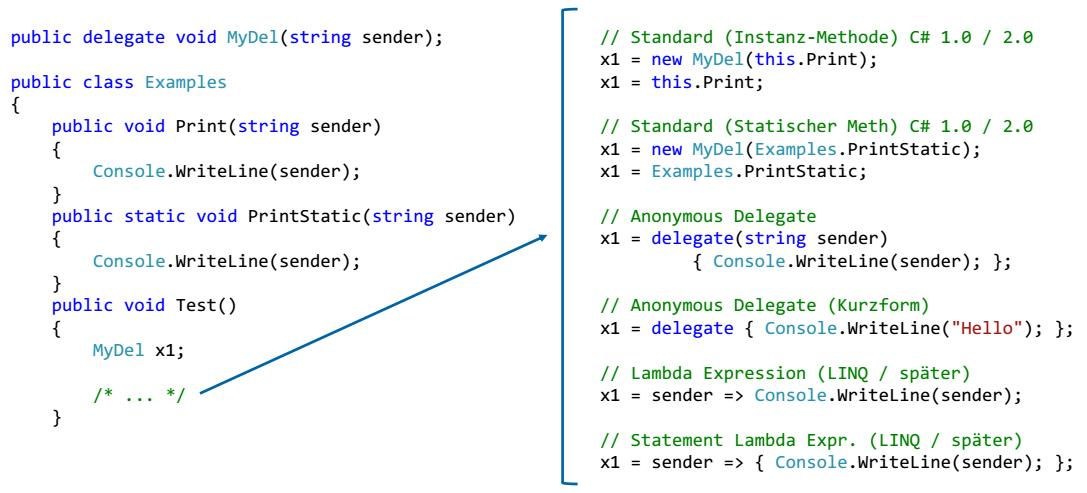
\includegraphics[width=0.9\linewidth]{images/delegate_lamda_overview}
	\caption{Delegate Lamda Overview}
\end{figure}

\subsection{Multicast Delegates}
Jedes Delegate ist auch ein Multicast Delegate. Im Unterschied zum normalen Delegate beinhaltet das Multicast Delegate mehrere Methoden. Weitere Methoden können mit += hizugefügt und mit -= wieder entfernt werden. Die Methode werden dann nacheinander aufgerufen. (Intern Linked List). Lamdas werden vom Compiler als Delegate abgebildet.  Speichert man den Rückgabewert bei der Ausführung des Delegates ab, entspricht dieser dem \textbf{Rückgabewert des letzten Funktionsaufruf}, sofern dieses ein Return-Value hatte.
\begin{lstlisting}
// keyword delegate
public delegate void Notifier(string sender);

class Examples {
	public void Test() {
		// Deklaration Delegate-Variable
		Notifier greetings; 
		// Zuweisung einer Methode mit passender Signatur
		greetings = new Notifier(SayHello); 
		// Kurzform
		greetings = SayHello;
		greetings += SayGoodBye;
		// Aufruf einer Delegate-Variable
		greetings("John");
	}

	private void SayHello(string sender) {
		Console.WriteLine("Hello {0}", sender);
	}
	
	private void SayGoodBye(string sender) {
		Console.WriteLine("Good bye {0}", sender);
	}
} 

// anonymous delegate
// inline multicast delegate
Calculator calc =  
	  delegate (int a, int b) { return a+b}
	+ delegate (int a, int b) { return a - b};
int res = calc(3,2) // 1 (last call)
\end{lstlisting}
\subsection{Funktionsparameter}
\begin{lstlisting}
public delegate void Action(int i);
public class MyClass
{
    public static void PrintValues(int i)
    { 
		Console.WriteLine("Value {0}", i);
	}
    public void SumValues(int i) { Sum += i; }
    public int Sum { get; private set; }
}
public class FunctionParameterTest
{
    static void ForAll(int[] array, Action action)
    {
        Console.WriteLine("ForAll called...");
        if (action == null) { return; }
        foreach (int t in array)
        {
            action(t);
        }
    }
}

public static void TestSum()
{
    MyClass c = new MyClass();
    int[] array = { 1, 5, 8, 14, 22 };
    
    // Delegate Variables
    Action v1 = c.PrintValues; // Static
    Action v2 = c.SumValues; // Instance Method
    
    // Execution
    ForAll(array, v1);
    ForAll(array, v1);
    
    ForAll(array, v2);
    Console.WriteLine("--- Sum {0}", c.Sum);
    ForAll(array, v2);
    Console.WriteLine("--- Sum {0}", c.Sum);
}
// Konsolen Ausgabe v1
ForAll called...
Value 1
Value 5
Value 8
Value 14
Value 22
ForAll called...
// Konsolen Ausgabe v2 
ForAll called...
--- Sum 50
ForAll called...
--- Sum 100
\end{lstlisting}
\begin{lstlisting}
public static void Test() {
    Action ToExecute;
    ToExecute = delegate(string str) { Console.WriteLine(str.ToLower());}; // Add toLower method
    ToExecute += delegate(string str) { Console.WriteLine(str.ToUpper());}; // add toUpper method
    ToExecute("Tubel"); //TUBEL tubel
}
\end{lstlisting}

\subsection{Anonyme Methoden}
Mit anonymen Methoden ist keine Deklaration einer Methode nötig. Methodencode wird in-place angegeben. Ebenfalls hat eine Methode Zugriff auf lokale Variablen (im unteren Beispiel \lstinline|sum|). \textbf{Besser mit Lambdas lösen!}

\begin{lstlisting}
class AnonymousMethods { 
    void Foo() { 
        list.ForEach(delegate(int i) { Console.WriteLine(i); } ); 
        int sum = 0; 
        list.ForEach(delegate(int i) { sum += i; } ); 
    }

} 
\end{lstlisting}

\subsection{Callbacks}
\textbf{Besser mit Events lösen!}
\begin{lstlisting}
public delegate void TickEventHandler (int ticks, int interval);

public class Clock
{
    private TickEventHandler OnTickEvent;

    public void add_OnTickEvent(TickEventHandler h)
    { OnTickEvent += h; }
    public void remove_OnTickEvent(TickEventHandler h)
    { OnTickEvent -= h; }
    private void Tick(object sender, EventArgs e)
    {
        ticks++;
        OnTickEvent?.Invoke(ticks, interval);
    }
}

public static void Test()
{
    Clock c1 = new Clock(1000);
    Clock c2 = new Clock(2000);
    
    ClockObserver t1 = new ClockObserver("O1");
    ClockObserver t2 = new ClockObserver("O2");
    
    //Observers anmelden
    c1.add_OnTickEvent(t1.OnTickEvent);
    c2.add_OnTickEvent(t2.OnTickEvent);
    
    // Warteschlaufe o.Ä
    
    //Observers abmelden
    c1.remove_OnTickEvent(t1.OnTickEvent);
    c2.remove_OnTickEvent(t2.OnTickEvent);
}
\end{lstlisting}

\clearpage
\subsection{Events}
Events sind Instanzen von Delegates, wobei das Delegate  implizit \lstinline|private| ist, damit es das Event nur von intern getriggert werden kann. (Kompiler Feature) Ein Event ist normalerweise \lstinline|void|. Events werden benötigt um zwischen Objekten zu kommunizieren. Ändert etwas in einem Objekt werden die andere benachrichtigt (Observer). Jeder Event verfügt über kompilergenerierte, öffentliche Add(+=) und Remove(-=) Methoden für das Subscriben von Methoden, Lamdas, etc.
\begin{lstlisting}
// 1. define delegate
public delegate void TimeEventHandler (object source, CustomEventArgs args);

// 2. define publisher
public class Clock {
	// 3. define an event based on delegate
	// compiles to private field with subscribe, unsubscribe methods
	public event TimeEventHandler OnTimeChangedEvent;
	
	public void MyAction() {
		// convetional name
		OnTimeChanged();
	}
	
	// 4. raise event
	protected virtual void OnTimeChanged() {
		CustomEventArgs args = new CustomEventArgs() {
			Custom = new custom(); // ref model
		}
		OnTimeChangedEvent?.Invoke(this, args)
	}
}

// 5. write subscribers
public class Subscriber {
	
	// match with delegate
	public void OnTimeChanged(object source, CustomEventArgs args) {
		/*... */ 
	}
}

//6. Event Args: Create 
public class CustomEventArgs : EventArgs {
	public Custom CustomProp { get; set; }
}

// Model
public class Custom {
	/*... */ 
}

// 7. use it
static void Main(string[] args) {
	var clock = new Clock(); // publisher
	var subscriber = new Subscriber(); // subscriber
	
	// add as many subscriber as needed
	clock.OnTimeChangedEvent += subscriber.OnTimeChanged;
	
	// 8. exec
	clock.MyAction();
}
\end{lstlisting}

\subsection{EventHandler}
Ein EventHandler hat folgende Eigenschaften:
\begin{description}
	\item[Standard Syntax] \lstinline|public delegate void AnyHandler(object sender, AnyEventArgs e); |
	\item [1. Parameter] \lstinline|object sender|:
	      \begin{itemize}
		      \item Sender des Events
		      \item Absender übergibt bei Aufruf des Delegates / Events \lstinline|this| mit
	      \end{itemize}
	\item [2. Parameter] \lstinline|AnyEventArgs e|:
	      \begin{itemize}
		      \item Beliebige Sub-Klasse von \lstinline|EventArgs|
		      \item Enthält Informationen zum Event (z.B. Linke oder Rechte Maustaste beim Klick, etc.)
		      \item Begründung: Argumente können jeder ergänzt werden ohne Anpassung der Signatur
	      \end{itemize}
\end{description}

Anstelle eines eigenen EventHandler kann man auch den bestehenden \lstinline|EventHandler<EventArgs>| nutzen.
\begin{lstlisting}[caption=C\# Event Handler]
public delegate void ClickEventHandler(obj sender, AnyEventArgs e);

public class ClickEventArgs : EventArgs {
	public string MouseButton{get; set;}
}

public class Button {
	public event ClickEventHandler OnClick;
}

public class Usage {
	public void Test() {
		Button b = new Button();
		// add custom click handler, must match delegate signature
		b.OnClick += OnClick;
	}
	
	// click handler
	private void OnClick(sender, ClickEventArgs eventargs) {
		/*...*/
	}
}
\end{lstlisting}

\section{Lambdas}
\begin{itemize}
	\item Lambdas können 0 oder mehrere Parameter haben
	\item Der Typ der Parameter darf weggelassen werden
	\item Man unterscheidet zwischen \textbf{Statement Lambdas} (Mit geschweiften Klammern) und \textbf{Expression Lambdas} (einzelner Ausdruck, kein return nötig). Ein Lambda kann als \lstinline|Func<>| Typ gespeichert werden.
\end{itemize}

\begin{lstlisting}
// Prototype
Func<[param_type], [return type]> myLamda;

// Expression Lambda
Func<int, bool> fe = i => i % 2 == 0;

// Statement Lambda
Func<int, bool> fs = i => {
	int rest = i%2;
	bool isRestZero = rest == 0;
	return isRestZero;
};

// Can be nested
Func<string, Func<string, int>> l = (string s) => ((string s2) => s2.Length);
var call = l("a")("b");
\end{lstlisting}

\subsection{Closure}
Der Zugriff auf lokale Variablen aus dem Lamda ist erlaubt.
\begin{lstlisting}
int x = 0;
Action a = () => x = 1;
Console.WriteLine(x); // Output: 0
a();
Console.WriteLine(x); // Output: 1
\end{lstlisting}

\begin{lstlisting}
// each lamda has its own instance of multiplier
public static Func<int, int> GetOp() {
	int multiplier = 2;
	Func<int, int> operator = x => x * multiplier++;
	return operator;
}

var operator = GetOp();
oper(2); // 4
GetOp()(2); // 4
oper(2) // 6
\end{lstlisting}


\section{Iteratoren}
Es sind mehrere Iteratoren zur gleichen Zeit auf eine Liste erlaubt. Die Collection darf während der Iteration nicht verändert werden.

\subsection{Foreach Loop}
Der Foreach Loop ist in C\# gleich wie in Java mit dem Unterschied, dass anstatt einem Dopplepunkt das Keyword \lstinline|in| verwendet wird. In C\# hat en \lstinline|foreach|-Loop folgende Besonderheiten:
\begin{itemize}
	\item \lstinline|continue| Unterbricht die aktuelle Iteration
	\item \lstinline|break| Unterbricht gesamten Loop
\end{itemize}
Die Collection, über welche geloopt wird, muss \lstinline|IEnumerable| rsp. \lstinline|IEnumberable<T>| implementieren. Eine andere Variante ist, dass die Collection einer Implementation von \lstinline|IEnumerable| rsp. \lstinline|IEnumberable<T>| ähneln muss. Das bedeutet konkret:
\begin{itemize}
	\item Collection hat Methode \lstinline|GetEnumerator()| mit Rückgabewert \lstinline|e|
	\item \lstinline|e| hat eine Methode \lstinline|MoveNext()| mit Rückgabewert \lstinline|bool|
	\item \lstinline|e| hat ein Property \lstinline|Current|
\end{itemize}

\begin{lstlisting}
int[] list = new int[] { 1, 2, 3, 4, 5, 6 };
foreach (int i in list) {
	if (i == 3) continue;
	if (i == 5) break;
	Console.WriteLine(i);
} // Ausgabe 1 2 4
\end{lstlisting}

\subsection{Iterator Interfaces}
Beim Thema Iteratoren haben wir zwei Interfaces, welche beteiligt sind:
\begin{enumerate}
	\item \lstinline|public interface IEnumberable| mit den Member:
	      \begin{itemize}
		      \item \lstinline|IEnumerator GetEnumerator()| gibt ein IEnumerator Objekt \lstinline|e| zurück.
	      \end{itemize}
	\item \lstinline|public interface IEnumerator| mit den Member:
	      \begin{itemize}
		      \item \lstinline|object Current { get; }| gibt aktuelles Element zurück
		      \item \lstinline| bool MoveNext();| springt zum nächsten Item
		      \item \lstinline| void Reset(); | Zurücksetzen des Iterators
	      \end{itemize}
\end{enumerate}
Diese Interfaces gibt es auch in generischer Form: \lstinline|Interface IEnumerable<T> : IEnumerable| und \lstinline|public interface IEnumerator<out T> : IDisponsable, IEnumerator|

\begin{lstlisting}
// each collection, which implements IEnumerable, supports foreach
public interface IEnumerable<out T> : IEnumerable {
	IEnumerator<T> GetEnumerator();
}

// IEnumerator
public interface IEnumerator<T> {
	T Current { get; }
	bool MoveNext(); // calls yield return
	void Reset();
}

public interface IEnumerator<out T> : IDisposable, IEnumerator {
	T Current { get; }
}
\end{lstlisting}


\subsection{Interator Methoden und Yield Return}
\begin{itemize}
	\item Eine Iterator Methode muss die Signatur \lstinline[]|public IEnumerator<int> GetEnumerator()| haben
	\item \lstinline|yield return| Statement gibt den nächsten Wert für die nächste Iteration eines \lstinline|foreach| Loops zurück
	\item muss \textbf{mindestens ein} \lstinline|yield return| Statement enthalten
	\item \lstinline|IEnumerator.MoveNext()| ruft den nächsten \lstinline|yield return| in \lstinline|GetEnumerator()| auf.
	\item \lstinline|yield break| terminiert die aktuelle Iteration
\end{itemize}
\begin{lstlisting}
class MyIntList {
	private int[] data = new int[10];
	
	// Standard Iterator
	public IEnumerator<int> GetEnumerator() {
		for (int i = 0; i < data.Length; i++) {
			yield return data[i];
		}
	}
	
	// Spezifische Iterator-Methode (Rueckgabewert = IEnumerable)
	public IEnumerable<int> Range(int from, int to) {
		for (int i = from; i < to; i++) {
			yield return data[i];
		}
	}
	
	// Spezifisches Iterator-Property (Rueckgabewert = IEnumerable)
	public IEnumerable<int> Reverse {
		get {
			for (int i = data.Length - 1; i >= 0; i--) {
				yield return data[i];
			}
		}
	}
	
	// Fibonacci
	public static IEnumerable<int> Fibonacci(int number) {
	 int a = 0, b = 1;
	 
	 yield return a;
	 yield return b;
	 
	 for (int i = 0; i <= number; i++)
	 {
		 int temp = a;
		 a = b;
		 b = temp + b;
		 yield return b;
	 }	 
	}
}
\end{lstlisting}

\begin{lstlisting}
MyIntList list = new MyIntList();

// Aufruf Standard Iterator
foreach (int elem in list) { .. }

// Aufruf spezifische Iterator Methode
foreach (int elem in list.Range(2, 7)) { .. }

// Aufruf Iterator Property
foreach (int elem in list.Reverse) { .. }
\end{lstlisting}

\clearpage

\section{Extension Methods}
\begin{itemize}
	\item Extension Methods erlauben das Erweitern (aus Anwendersicht) bestehender Klassen
	\item Extension Methoden können auf Klassen, Structs, Interfaces, Delegates, Enumeratore und Arrays angewendet werden.
	\item Extension Methods werden hauptsächlich für das Method Chaining verwendet.
	\item Eine Extension Method muss \textbf{statisch} sein und der erste Parameter der Methode \lstinline|this| als Prefix haben.
	\item Der erste Parameter definiert die Klasse, welche erweitert wird
	\item Kein Zugriff auf interne Members aus Extension Methode
\end{itemize}

\begin{lstlisting}[language={[Sharp]C}]
 public static class ExentsionMethods
    {
        public static string ToStringSafe(this object current)
        {
            return current == null ? string.Empty : current.ToString();
        }
    }
\end{lstlisting}
\subsection{Deferred Evaluation}
Der Aufruf von einer Methode, welche einen \lstinline|IEnumerator| zurückgibt, führt diesen \textbf{noch nicht} aus.
Dies passiert erst implizit im foreach-loop.
Mit dem Verwenden von Extension Methods mit Iterationen kann so eine Query-Operation implementiert werden, welche verschachtelt werden kann. Diese haben folgende Eigenschaften:
\begin{itemize}
	\item Erweitern alle Collections die IEnumerable implementieren
	\item Liefern in der Regel wieder ein IEnumerable
	\item Können mit dem "."-Operator verkettet werden
	\item Werden "deferred" (aufgeschoben) evaluiert
\end{itemize}
Mit dem this-Kontext, welcher der Extension Methode mitgegeben wird, macht man die Verbindung zu der Collection.

\begin{lstlisting}
public static class MyExtensions {
	public static IEnumerable<T> OstWhere<T> (this IEnumerable<T> source, Predicate<T> predicate) {
		foreach (T item in source) {
			if (predicate(item)) {
				yield return item;
			}
		}
	}
	
	public static IEnumerable<T> OstOfType<T> (this IEnumerable source) {
		foreach (object item in source) {
			if (item is T ) {
				yield return (T)item;
			}
		}
	}
}

// Anwendung

object[] list = { 4, 3.5, "abc", 3, 6 };
// Extension Method Syntax 
IEnumerable<int> res = list
                       .HsrOfType<int>()
                       .HsrWhere(delegate (int k) { return k % 2 == 0; }); 
\end{lstlisting}

\section{Exceptions}
Wie auch in anderen Sprachen behandeln Exceptions unerwartete Programmstati oder Ausnahmeverhalten zur Laufzeit. Sie sind Fehlercodes vorzuziehen.

Es wird pro Exception nur ein catch-Block ausgeführt. Jede Exception muss von System.Exception erben. Es gibt keine \lstinline|throws| Anmerkung am Methoden Kopf.
In C\# sind alle Exception Unchecked Exceptionn (müssen nicht behandelt werden.)
\begin{lstlisting}
try {
    // code to execute
} catch (FileNotFoundException e) {
} catch (IOException) {
	// optional var name, if not needed
} catch {
	// implizit System.Exception
} finally {
	// always executed
}

// throw exception
throw new Exception("An error occured");
throw new ArgumentNullException(nameof(s)); // nameof zur Ermittlung des ungültigen Parameter

// exception weiterwerfen ( neuen Stack Trace)
catch (Exception e) { throw e; }

// rethrowing (Stack Trace bleibt erhalten)
catch (Exception e) { throw; } 
\end{lstlisting}


\begin{figure}[ht]
	\centering
	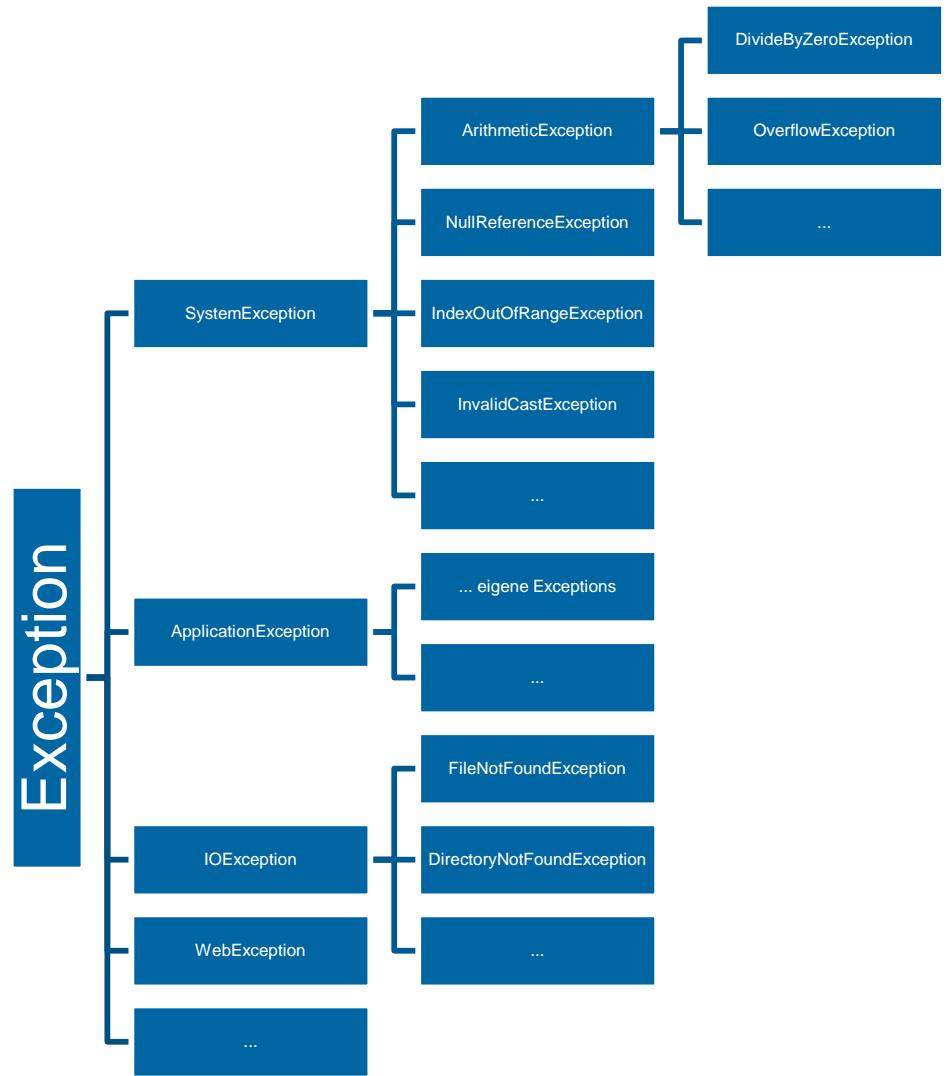
\includegraphics[width=\linewidth]{images/exception_classes}
	\caption{Exception Klassen}
	\label{fig:exceptionclasses}
\end{figure}

\subsection{Exception Filter}
Exception Filters sind Catch-Blöcke, welche nur unter definierten Bedingungen ausgeführt werden. Es sind \lstinline|when| Klauseln, welche einen \lstinline|bool| Expression erwarten.
\begin{lstlisting}
try {
} catch (Exception e) when (DateTime.Now.Hour < 18) {
} catch (Exception e) when (DateTime.Now.Hour >= 18) {}
\end{lstlisting}

\section{Direct Initialization}

\subsection{Object Initializers}
Object Initialisierer erlaubt das Instanzieren und Initialisieren einer Klasse in einem einzigen Statement. Die Objekte lassen sich auch erzeugen, wenn kein passender Konstruktor zur Verfügung steht.
\begin{lstlisting}
	Student s1 = new Student("John") {
		Id = 2009001,
		Subject = "Computing"
	};
	Student s2 = new Student {
		Name = "Ann",
		Id = 2009002,
		Subject = "Mathematics"
	};
	
	// Object Initializers zusammen mit Lamdas
	int[] ids = { 2009001, 2009002, 2009003 };
	IEnumerable<Student> students = ids.Select(n => new Student { Id = n });
\end{lstlisting}

\subsection{Collection Initializers}
Ist das selbe wie Objekte Initializers, jedoch mit Listen.
\begin{lstlisting}
	List<int> l1 = new List<int> { 1, 2, 3, 4 };
	Dictionary<int, string> d1 = new Dictionary<int, string>
	{
		{ 1, "a" },
		{ 2, "b" },
		{ 3, "c" }
	};
	d1 = new Dictionary<int, string> {
		[1] = "a",
		[2] = "b",
		[3] = "c"
	};
	
	object s = new Dictionary<int, Student>
	{
		{ 2009001, new Student("John") {
				Id = 2009001,
				Subject = "Computing" } },
		{ 2009002, new Student {
				Name = "Ann", Id = 2009002,
				Subject = "Mathematics" } }
	};
\end{lstlisting}
\subsection{Kombination aus Object und Collection Initializers}
//Kombination Object und Collection Initializers
\begin{lstlisting}
object s = new Dictionary < int, Student >
{
  {
       2009001,
       new Student("John") {
        Id = 2009001, Subject = "Computing"
       }
  },
  {
      2009002,
      new Student {
        Name = "Ann", Id = 2009002, Subject = "Mathematics"
      }
  }
};
\end{lstlisting}

\subsection{VAR: Anonymous Types}
\begin{itemize}
	\item Mit dem Schlüsselwort \lstinline|var| wird der Typ vom Compiler herausgefunden
	\item \lstinline|var| kann nur für lokale Variablen verwendet werden. Der Einsatz bei Parametern, Klassenvariablem und Properties ist nicht erlaubt.
	\item Der Typ wird aus der Zuweisung abgeleitet, wobei die Variable zu 100\% typensicher bleibt.
	\item Wird meistens in LINQ Queries verwendet (um Zwischenresultate zu speichern)
	\item \textbf{Wichtig:} Properties von Anonymen Typen sind immer readonly.
\end{itemize}

\begin{lstlisting}
class Student {
 public string Name;
 public int Id;
 public string Subject {
  get;
  set;
 }
 public Student() {}
 public Student(string name) {
  Name = name;
 }
}
public class Examples {
 public void Test() {
  var a = new {
   Id = 1, Name = "John"
  };
  var b = new {
   a.Id, a.Name
  };
  var studentList = new List < Student > ();
  var q = studentList.GroupBy(s => s.Subject).Select(grp => new {
   Subject = grp.Key, Count = grp.Count()
  });
 }
}
\end{lstlisting}

\section{LINQ: Language Integrated Query}
LINQ erlaubt eine Query Syntax um Abfragen an beliebigen Datenstrukturen zu machen. Man unterscheidet den Extension- und Query Expression Syntax (Erinnert an SQL), wobei beide die gleichen Dinge erlauben. (Sie erzeugen den selben \textit{msil} Code) Auch LINQ ist reines Compiler Feature.

\begin{figure}[ht]
	\centering
	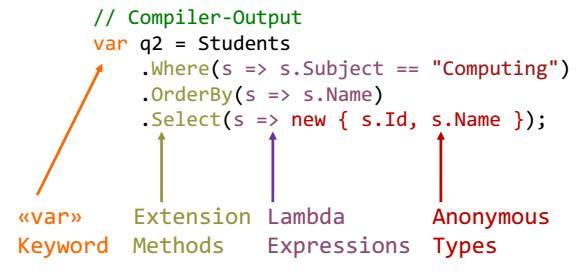
\includegraphics[width=0.7\linewidth]{images/linq_components}
	\caption{LINQ Komponenten}
	\label{fig:linqcomponents}
\end{figure}

\begin{lstlisting}
// Query expression syntax
var empQuery =
        from e in employees
        from d in departments
        where e.DepId == d.Id
        orderby d.Name
        select new { EmployeeName = e.Name, DepartmentName = d.Name };

// Extension Method / Lamda syntax
var empQuery = employees
.Join(departments, 
	eKey => eKey.DepId, 
	dKey => dKey.Id, (e, d) => new { 
		EmployeeName = e.Name, 
		DepartmentName = d.Name })
.OrderBy(k1 => k1.DepartmentName);

// Query expression syntax
var projList = from p in projects
from e in p.Employees
orderby p.Name, e.Name
select new { Project = p.Name, Employee = e.Name };

// Extension Method / Lamda syntax
var projList = projects
    .SelectMany(p => p.Employees
        .Select(e => new { Project = p.Name, Employee = e.Name }))
    .OrderBy(p => p.Project)
    .ThenBy(p => p.Employee);			  
\end{lstlisting}
\subsection{Lambda Expressions}
Eine Lambda Expression ist eine anonyme Methode mit folgende Eigenschaften:
\begin{itemize}
	\item Keine Implementation einer benannten Methode nötig
	\item \lstinline|delegate| Schlüsselwort fällt weg
	\item Angaben von Parametertypen optional
	\item Kann auf äussere Variablen zugreifen, aber nicht umgekehrt
	\item Zwei Ausprägungen
	      \begin{itemize}
		      \item Expression Lambdas (nicht im Klammern gefasst, genau ein Ausdruck): \lstinline|(parameters) => expression|
		      \item Statement Lambdas (Beliebig viele Statements in Block gefasst) \lstinline|(parameters) => { statements; }|
	      \end{itemize}
\end{itemize}

\subsection{Extension Methods und Deferred Evaluation}
Query Operationen sind ebenfalls mit \lstinline|yield return| implementiert. Das bedeutet geben ein \lstinline|IEnumerable<T>| zurück, welches nicht direkt ausgeführt wird. Da es nicht direkt ausgeführt sondern zurückgeschoben wird, spricht man auch von Deffered Evaluation. Daher können die Resulatate immer anders sein.

\begin{lstlisting}
public void TestDeferredEvaluation(){
 string[] cities = { "Bern", "Basel", "Zürich", "Rapperswil", "Genf" };
 IEnumerable<string> citiesB = cities.Where(c => c.StartsWith("B"));
 // Ausführung: 2 Städte (Bern, Basel)
 foreach (string c in citiesB) { /* ... */ } 
 cities[0] = "Luzern"; 
 // Ausführung: 1 Stadt (Basel)
 foreach (string c in citiesB) { /* ... */ }
} 
\end{lstlisting}

\subsection{Extension Methods und Immediate Evaluation}
Einige Operatoren führen Queries direkt aus (in der Regel wenn der Rückgabewert nicht IEnumerable ist). Resultate werden direkt in Variable gespeichert
\begin{itemize}
	\item ToList / ToArray
	\item Count / First
	\item Sum / Average
\end{itemize}
\begin{lstlisting}
public void TestDeferredEvaluation()
{
    string[] cities = { "Bern", "Basel", "Zürich", "Rapperswil", "Genf" };
    // Ausführung
    List<string> citiesB = cities.Where(c => c.StartsWith("B")).ToList();
    int citiesEndl = cities.Where(c => c.EndsWith("l")).Count();
}
\end{lstlisting}


\subsection{Extensions Syntax (Fluent Syntax)}
\subsubsection{LINQ Extension Methods}
LINQ bringt in der Klasse \lstinline|Enumerable| eine Vielzahl an Query Operatoren wie \lstinline|Where(), OrderBy(), etc.| mit sich. Innerhalb der Extension Method kann dann ein z.B ein Lamda übergeben werden. (Predicate)

\begin{lstlisting}
// needs to be static class
public static class Extensions {

	// should be generic
	public static void HsrForEach<TSource>(this IEnumerable<TSource> source, Action<TSource> action) {
		foreach (TSource item in source) {
			action(item);
		}
	}

	public static IEnumerable<TSource> HsrWhere<TSource>(this IEnumerable<TSource> source, Func<TSource, bool> predicate) {
		foreach (TSource item in source) {
			if (predicate(item)) {
				// use yield return
				yield return item;
			}
		}
	}
	
	// use yield, because we return IEnumerable
	public static IEnumerable<TResult> HsrOfType<TResult>(this IEnumerable source) {
		foreach (object item in source) {
			if (item is TResult) {
				yield return (TResult)item;
			}
		}
	}
	
	public static List<TSource> HsrToList<TSource>(this IEnumerable<TSource> source) {
		return new List<TSource>(source);
	}
	
	public static int HsrSum<TSource>(this IEnumerable<TSource> source, Func<TSource, int> selector) {
		int sum = 0;
		foreach (TSource t in source) {
			sum += selector(t);
		}
		return sum;
	}
} 
\end{lstlisting}
\subsubsection{SelectMany}
SelectMany erleichert das zusammenfassen verschachtelter Listen.
\begin{lstlisting}
var projList = projects
	.SelectMany(p => p.Employees
	.Select(e => new { Project = p.Name, 
	Employee = e.Name }))
	.OrderBy(p => p.Project)
	.ThenBy(p => p.Employee);
\end{lstlisting}


\subsection{Query Expressions Syntax}
\begin{lstlisting}
//  1. Datenquelle waehlen
int[] numbers = { 0, 1, 2, 3, 4, 5, 6 };

// 2. Query erstellen
var numQuery = from num in numbers
	where (num % 2) == 0
	select num;

// 3. Query ausfuehren
foreach (int num in numQuery) {
	Console.Write("{0,1} ", num);
}
\end{lstlisting}

\begin{itemize}
	\item from: Datenquelle
	\item where: Filter
	\item orderby: Sortierung
	\item select: Projektion
	\item group:  Gruppierung in eine Sequenz von Gruppen Elementen
	\item join: Verknüpfung zweier Datenquellen
	\item let: Definition von Hilfsvariablen
\end{itemize}
\textbf{Grundregeln:} Query Syntax beginnt immer mit \lstinline|from| und Query Syntax endet immermit \lstinline|select| oder \lstinline|group|
\begin{figure}[ht]
	\centering
	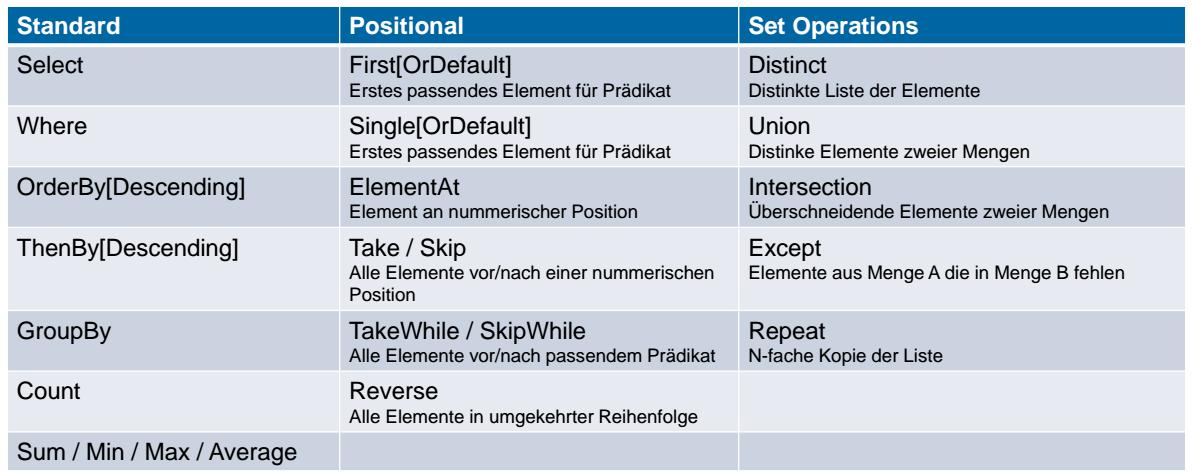
\includegraphics[width=\linewidth]{images/linq_query_operatoren}
	\caption{Query Operatoren}
	\label{fig:linqqueryoperatoren}
\end{figure}

\newpage

\subsubsection{Range Variabeln}
Range Variabeln entstehen durch \lstinline|from| oder \lstinline|join| oder \lstinline|into| und sind readonly.
Im folgenden Beispiel sind die Variabeln s, m und g Range Variabeln:
\begin{lstlisting}
from s in Students
join m in Markings on s.Id equals m.StudentId
group s by s.Subject into g 
select g; 
\end{lstlisting}

\subsubsection{Gruppierung}
Transformation in Key/Value Pairs:
\begin{lstlisting}
// q: IEnumerable<IGrouping<string, string>>
var q = from s in Students
group s.Name by s.Subject;
foreach (var group in q)
{
	Console.WriteLine(group.Key);
	foreach (var name in group)
	{
		Console.WriteLine("  " + name);
	}
}

// Gruppierung mit direkter Weiterverarbeitung mittels into
var q = from s in Students
	group s.Name by s.Subject into g
	select new {
		Field = g.Key,
		N = g.Count()
	};

foreach (var x in q) {
	Console.WriteLine(x.Field + ": " + x.N);
}


// Anz. Bestellungen pro Datum
from best in Bestellungen
group best by best.Datum into datumGroup
orderby datumGroup.Key
select new {
	Datum = datumGroup.Key,
	Anzahl = datumGroup.Count()
};

\end{lstlisting}

\clearpage

\subsubsection{Inner Joins}
Ein Inner Join nimmt nur jene Ergebnisse, die nicht \lstinline|null| sind.
Es werden zwei Mengen über einen Schlüssel verknüpft.
\textbf{Wichtig: } \lstinline|equals| nicht == verwenden.
\begin{lstlisting}
var q = from s in Students
	join m in Markings on s.Id equals m.StudentId
	select s.Name + ", " + m.Course + ", " + m.Mark;
\end{lstlisting}

\subsubsection{Group Joins}
Ein Group Join verwendet die \lstinline|into| Expression. s bleibt sichtbar
\begin{lstlisting}
// Pro "Student" wird eine Liste für alle "Markings" erstellt 
var q =
	from s in Students
	join m in Markings on s.Id equals m.StudentId
	into list
	select new
	{
		Name = s.Name,
		Marks = list
	};
	
foreach (var group in q) {
	Console.WriteLine(group.Name);
	foreach (var m in group.Marks) {
		Console.WriteLine(m.Course);
	}
}
\end{lstlisting}

\subsubsection{Left Outer Joins}
Verknüpft zwei Mengen über einen Schlüssel. Wenn kein rechtes Element gefunden wird bleibt linkes Element trotzdem bestehen.
\begin{lstlisting}
var q = from s in Students
	join m in Markings on s.Id equals m.StudentId into match
	from sm in match.DefaultIfEmpty()
	select s.Name + ", " + (sm == null
		? "?"
		: sm.Course + ", " + sm.Mark);
		
foreach (var x in q) {
	Console.WriteLine(x);
}
\end{lstlisting}

\begin{lstlisting}
var data = from fd in FlightDetails
join pd in PassengersDetails on fd.Flightno equals pd.FlightNo into joinedT
from pd in joinedT.DefaultIfEmpty()
select new {
	nr = fd.Flightno,
	name = fd.FlightName,
	passengerId = pd == null ? String.Empty : pd.PassengerId,
	passengerType = pd == null ? String.Empty : pd.PassengerType
}
\end{lstlisting}

\clearpage

\subsubsection{Let}
Let erlaubt das Definieren von Hilfsvariablen
\begin{lstlisting}
var result =
	from s in Students
	let year = s.Id / 1000
	where year == 2009
	select s.Name + " " + year.ToString();

foreach (string s in result) {
	Console.WriteLine(s);
}
\end{lstlisting}


\subsubsection{Select Many}
Man spricht von Select Many im Query Syntax, wenn das zweite \lstinline|from| sich auf das Erste bezieht.
\begin{lstlisting}
var selectMany = from a in MyArray
	from b in a.Split() // another array
	select b;
\end{lstlisting}

\subsubsection{Left Outer Join mit Select Many}
\begin{lstlisting}
var projList = 
	from p in projects
	from pl in p.ProjectManager.DefaultIfEmpty()
	orderby p.Name
	select new { 
		Project = p.Name,
		Manager = (pl==null) ? "-" : pl.Name 
	};
\end{lstlisting}

\section{Expression-Bodied Members}
Anstelle von einem Block{} können Expression-Bodied Members verwendet werden. Jedoch dürfen die Blöcke maximal ein Statement enthalten. Das Ganze funktioniert für Methoden/Operatoren, (De-)Konstruktoren, Properties/Indexers.
\begin{lstlisting}
public class Examples {
 private int value;
 // Constructors / Destructors (C# 7.0)
 public Examples(int value) => this.value = value;
 ~Examples() => this.value = 0;
 // Methods (C# 6.0) 
 public int Sum(int x, int y) => x + y;
 public int GetZero() => 0;
 public void Print() => Console.WriteLine("Hello");
 // Properties (C# 6.0) 
 public int Zero => 0;
 public int Bla => Sum(Zero, 2);
 // Getters/Setters (C# 7.0) 
 public int Value {
  get => this.value;
  set => this.value = value;
 }
}
\end{lstlisting}
\section{Tasks}
Ein Task ist eine leichtgewichtige Variante eines Threads und repräsentiert eine asynchrone Operation. Synchrone Waits sind \textbf{gefährlich} und \textbf{blockieren} den aktuellen Thread! Beispielsweise kann ein Download den ganzen Thread für eine bestimmte Zeit blockieren. Besser mit  \lstinline|async|/ \lstinline|await| arbeiten.
\begin{lstlisting}
Task task = Task
    .Run( 
        () => { /* Some workload */ }
    )
    .ContinueWith( t => 1234 );
    task.Wait();
\end{lstlisting}
\subsection{Task vs Thread}
\begin{minipage}[t]{1\textwidth}
	\centering
	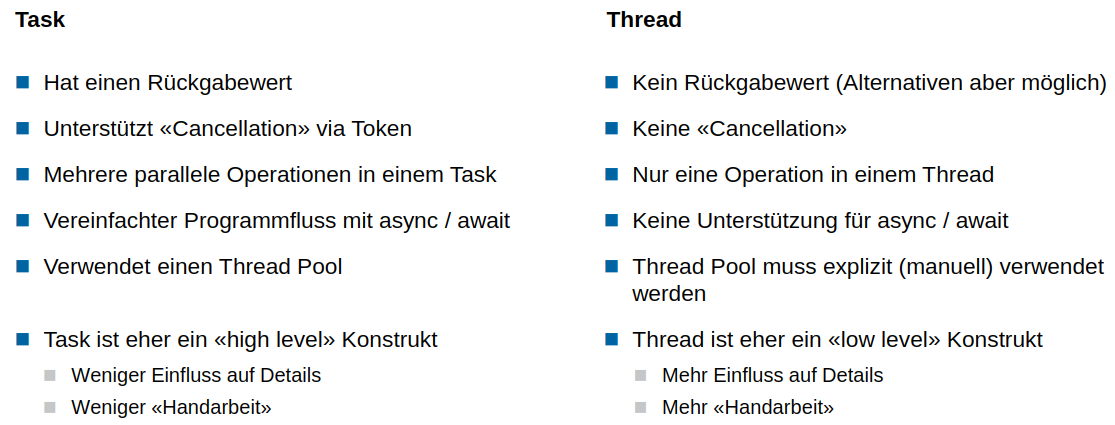
\includegraphics[width=1\linewidth]{images/task_vs_thread.png}
\end{minipage}
\subsection{Task API (synchrone waits)}
\begin{minipage}[t]{1\textwidth}
	\centering
	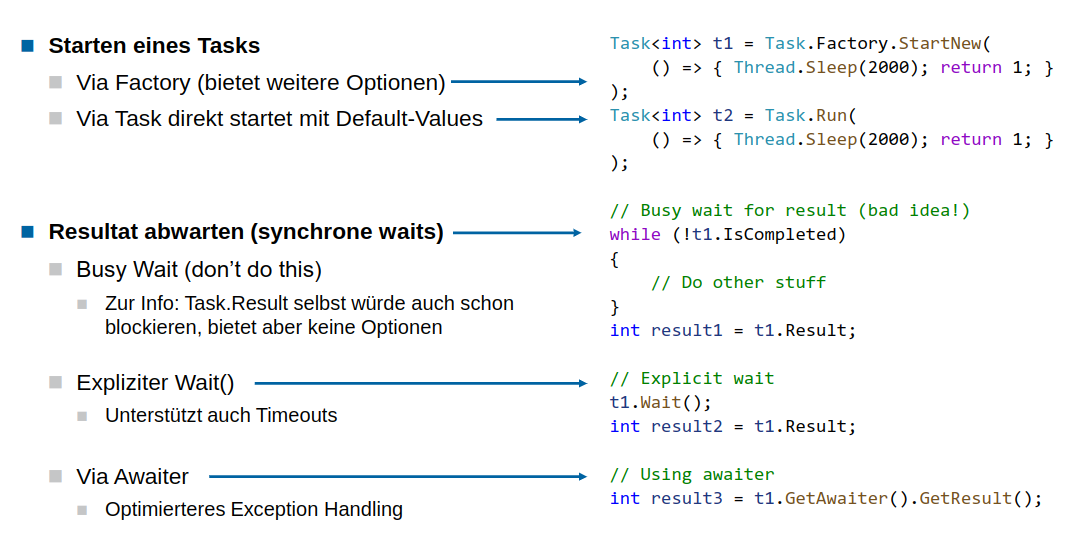
\includegraphics[width=1\linewidth]{images/task-api.png}
\end{minipage}

\section{ASYNC / AWAIT}
\subsection{Synchron vs. Asynchron}
\paragraph{Synchrone Operation}
\begin{itemize}
	\item Return aus der Methode nachdem die gesamte Logik durchlaufen wurde
	\item Blockieren den aktuellen Thread bis diese fertig gelaufen sind
\end{itemize}
\paragraph{Asynchrone Operation}
\begin{itemize}
	\item Ruft eine Methode auf ohne auf das Resultat zu warten
	\item Möglichkeit zur Benachrichtigung bei Fertigstellung (Callback)
	\item Oder: Rückgabe eines \lstinline|Task| Objektes auf welchem Status abgefragt werden kann
\end{itemize}
\subsection{async / await}
\paragraph{async}
\begin{itemize}
	\item Markiert die Methode als asynchron
	\item Einschränkung Rückgabewert
	      \begin{itemize}
		      \item Task (Task ohneRückgabewert)
		      \item Task<T> (Task mit Rückgabewert T)
		      \item void (Fire and forget, i.d.R nicht verwendet)
	      \end{itemize}
\end{itemize}
\paragraph{await}
\begin{itemize}
	\item Alles nach 'await' ist wird vom Compiler zu einer 'Continuation' umgewandelt (es wird also nicht blockiert)
	\item Nur in 'async' Methoden erlaubt
\end{itemize}
\clearpage
\paragraph{Beispiel / Download Content mit await} \hfill
\newline


\begin{minipage}[t]{0.95\textwidth}
	\centering
	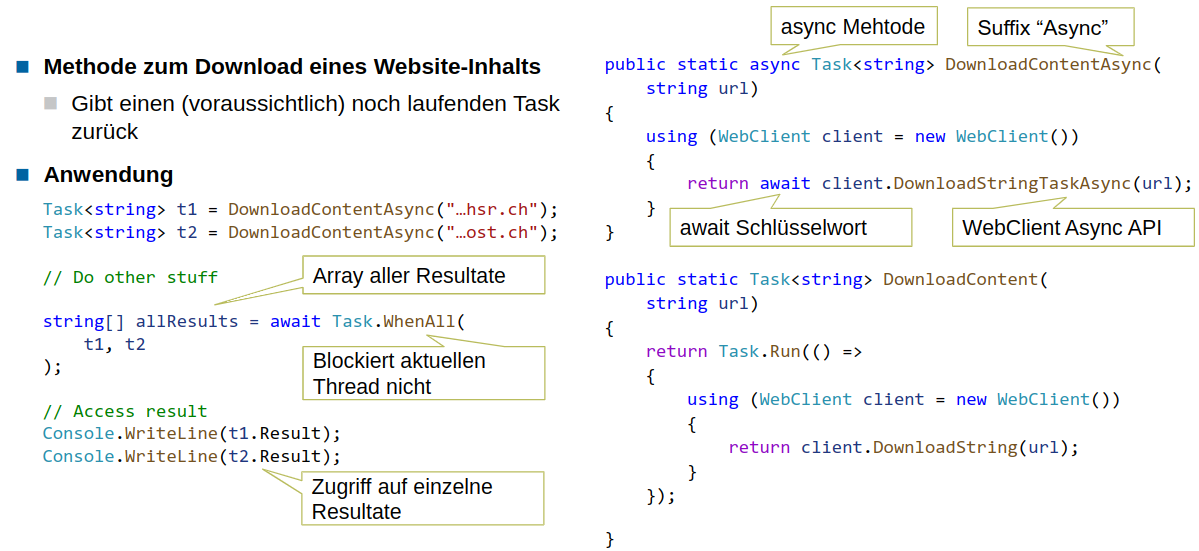
\includegraphics[width=0.95\linewidth]{images/beispiel-async-await.png}
\end{minipage}

\paragraph{Vor- und Nachteile async/await}
\begin{itemize}
	\item[+] Code sieht immer noch synchron aus
	\item[+] Keine Continuations nötig
	\item[+] Ersetzt Multithreading für asynchrone Ausführungen
	\item[-] Overhead is relativ gross
	\item[-] Lohnt sich daher erst bei längeren Operationen
	\item[-] Await nicht erlaub in lock-Statements
\end{itemize}

\subsection{Cancellation}
Integriertes Programmiermodell für das Abbrechen von Programmlogik, z.B. Abbruch einer langlaufenden Datenbankoperation, wenn API-Call abgebrochen wurde oder ein Abbruch durch 'CTRL+C'.

Nutzt die Klasse \lstinline|CancellationToken|. Muss durch die gesamte Aufrufkette durchgereicht werden. Dies als letzter Parameter jeder asynchroner Methode (Best Practices).

\begin{lstlisting}
static void ManualCancellation(
	CancellationToken cancellationToken)
	{
	for (int i = 0; i < 100_000; i++)
	{
		// Do some work...

		// Variante A
		if (cancellationToken.IsCancellationRequested) { /* ... */ }

		// Variante B
		cancellationToken.ThrowIfCancellationRequested();
	}
}
\end{lstlisting}

\subsubsection{Cancellation Token Source}
Klasse zur Erstellung und Steuerung von CancellationTokens. Kann beliebig viele Tokens emittieren.
\begin{lstlisting}
CancellationTokenSource cts = new();
CancellationToken ct = cts.Token;

Task t1 = LongRunning(1_000, ct); // 1s tied to CTS
Task t2 = LongRunning(3_000, ct); // 3s tied to CTS
Task t3 = LongRunning(3_500, default); // 3s independent/not cancellable

await Task.Delay(2_000, ct);

Console.WriteLine("Cancelling");
cts.Cancel();
Console.WriteLine("Canceled");

async Task LongRunning(int ms, CancellationToken ct)
{
	Console.WriteLine($"{ms}ms Task started.");
	await Task.Delay(ms, ct);
	Console.WriteLine($"{ms}ms Task completed.");
};

//Console output:
//-----------------------
//1000ms Task started.
//3000ms Task started.
//3500ms Task started.
//1000ms Task completed.
//Cancelling
//Canceled
//3500ms Task completed.
\end{lstlisting}

\section{Entity Framework}
Entity Framework Core /EF Core ist ein O/R Mapping Framework und verbindet Objekt-Orientiertes (Domain Model) mit Relationalem (Relational Model). Man unterscheidet zwischen zwei Varianten wie die Entitätsklassen/Datenbanken erstellt werden könnnen.
\paragraph{Basis-Funktionalitäten} Mapping von Entitäten, CRUD Operationen, Key-Generierung, Caching, Change Tracking, Optimistic Concurrency, Transactions, CLI
\begin{description}
	\item[DB First] Man erstellt zuerst ein Domain Model und generiert daraus die Klassen. Man kann das Model auch von einer existierenden Datenbank ableiten und dann wieder die Klassen daraus generieren
	\item[Code First] Man erstellt die Model Klassen und lässt die Datenbank automatisch generieren.
	\item[Model First] Man erstellt zuerst das EDM (Entity Data Model) und generiert daraus die Database, sowie die Klassen
\end{description}

\subsection{OR Mapping}
Ein OR-Mapper (Mapping) stellt die Verbindung zwischen Datenbank (Storage Entity) und Klassen (Entity Type) her. Er verbindet die Object ID mit dem Primary Key und bildet auch komplexer gebilde, wie z.B Vererbung ab. Beim Code First Ansatz \textbf{muss ein Member Id rsp. [ClassName]Id} existieren, damit das Entity Framework über den PrimaryKey bescheid weiss.
\begin{description}
	\item[Providers] Diverse relationale SQL Providers. (Von NuGet)
	\item[Entity] Ein Objekt mit einem Key (z.B ID). Mehrere dieser Objekte werden zu einem Entity-Set zusammengefasst.
	\item[Mapping] Mapping der Klassen auf das darunter liegende Speichermodell.
	\item[Mappingansätze] \textbf{By Convention}, \textbf{By Attributes}, \textbf{By Fluent API} . Zuordnung von Entity Type zu Storage Entity, Property zu Column, Entity Key zu Primary Key, Foreign Key zu Relationship.
	\item[Storage Entity] Relationales Modell/Graph/Collection, abhängig vom gewählten Provider. Ausprägungen: Table, View, Sotrec Procedures, etc. Inhalte: Columns, Primary KEys, Unique Key Constraints, Foreign Keys.
	\item[Association] Definiert eine Assotiation zwischen Entitäten (z.B Navigation Properties, Foreign Keys).
\end{description}

\begin{figure}[ht]
	\centering
	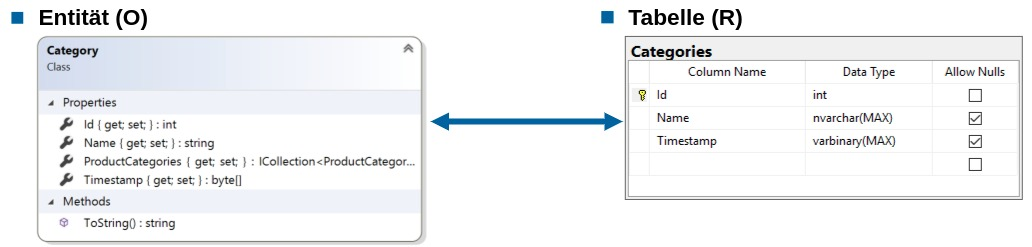
\includegraphics[width=0.8\linewidth]{images/entityframework_or_mapping.png}
	\caption{OR Mapping Entität <-> Tabelle}
	\label{fig:entityframeworkormapping}
\end{figure}
\begin{lstlisting}
using (ShopContext context = new ShopContext()) {
    var query = from c in context.Categories                            SELECT TOP(2)
        where c.Name == "Tablets"                                           [c].[Id], [c].[Name], [c].[Timestamp]
        select c;                                                       FROM [Categories] AS [c]
    Category tablets = query.Single()                                   Where [c].[Name] = N'Tablets'
}                                               // ------------>
\end{lstlisting}

\subsubsection{Modell}
\begin{description}
	\item[Convention] Automatisches Mapping ohne explizite Konfiguration.
	\item[Fluent API] Extensions Method Syntax, Überschriebene Methode von ''OnModelCreating'' im DbContext \lstinline|protected override void OnModelCreating(ModelBuilder modelBuilder)|.
	\item[Data Annotations|Attributes] Deklaratives Mapping, Attribute direkt auf Model-Klassen
\end{description}

\textbf{Mapping Ansätze:} Database First, Model First, Code First

In den nachfolgenden Beispiele sind jeweils 3 Arten von komplementären Mappings vermischt. Gleiche Mappings werden mehrfach in verschiedenen Arten gezeigt.

\paragraph{Include/Exclude Entities}
\begin{lstlisting}
public class ShopContext : DbContext {
    // Convention - DbSet-Property im Context
    public DbSet<Category> Categories { get; set; }
    
    // Fluent API - Entry im Builder oder Ignore im Model Builder
    protected override void OnModelCreating( ModelBuilder modelBuilder) {
        modelBuilder.Entity<AuditEntry>();          
        modelBuilder.Ignore<Metadata>();
    }
}
public class Category {
    public int Id { get; set; }
    public string Name { get; set; }
    public ICollection<Product> Products { get; set; }  // Convention - Indirekt via Navigation Property
    public ICollection<Metadata> Metadata { get; set; }
}
public class Product { /* ... */ }
public class AuditEntry { /* ... */ }
[NotMapped]                                               // Data Annotations
public class Metadata { /* ... */ }
\end{lstlisting}

\paragraph{Include/Exclude Properties}
Convention: Alle public Properties mit Getter/Setter
\begin{lstlisting}
public class ShopContext : DbContext {
    public DbSet<Category> Categories { get; set; }
    protected override void OnModelCreating(ModelBuilder modelBuilder) {
        modelBuilder.Entity<Category>()
            .Property(b => b.Name);                     
        modelBuilder.Entity<Category>()
            .Ignore(b => b.LoadedFromDatabase);             // Fluent API - Ignore im Builder
    }
}
public class Category {
    public int Id { get; set; }
    public string Name { get; set; }
    [NotMapped]                                               // Data Annotations
    public DateTime LoadedFromDatabase { get; set; }
}
\end{lstlisting}

\paragraph{Keys}
Convention: Property mit dem Namen ''[Entity]Id'' (z.b. Category.Id, Category.CategoryId)
\begin{lstlisting}
public class ShopContext : DbContext {
    public DbSet<Category> Categories { get; set; }
    protected override void OnModelCreating(ModelBuilder modelBuilder) {
        modelBuilder.Entity<Category>()
            .HasKey(e => e.Id)                              // Fluent API - Einzige Moeglichkeit für Composite Keys
            .IsRequired();
    }
}
public class Category {
    [Key]                                                   // Data Annotations
    public int Id { get; set; }
    public string Name { get; set; }
}
public class Tanslation {
    public string Language { get; set; }
    public int CategoryId { get; set; }
}
\end{lstlisting}

\paragraph{Required / Optional}
Convention: Value Types werden ''NOT NULL'' (int), Nullable Value Types werden ''NULL'' (int?), Reference Types werden ''NULL''
\begin{lstlisting}
public class ShopContext : DbContext {
    public DbSet<Category> Categories { get; set; }
    protected override void OnModelCreating(ModelBuilder modelBuilder) {
        modelBuilder.Entity<Category>()
            .Property(e => e.Name)
            .IsRequired();                              // Fluent API
    }
}
public class Category {
    public int Id { get; set; }
    [Required]                                          // Data Annotations
    public string Name { get; set; }
    public bool? IsActive { get; set; }
}
\end{lstlisting}

\paragraph{Maximum Length}
Convention: Keine Restriktion / z.b. NVARCHAR(MAX), 450 Zeichen bei Keys
\begin{lstlisting}
.Property(e => e.Name).HasMaxLength(500)                 // Fluent API
[MaxLength(500)]                                         // Data Annotations
\end{lstlisting}

\paragraph{Unicode}
Convention: Strings sind immer Unicode (NVARCHAR)
\begin{lstlisting}
.Property(e => e.Name).isUnicode(false)                 // Fluent API
[Unicode(false)]                                        // Data Annotations
\end{lstlisting}

\paragraph{Precision}
Convention: Pro Datentyp im Provider festgelegt, Precision: Genauigkeit / Anzahl digits total, Scale: Anzahl Nachkommastellen
\begin{lstlisting}
.Property(e => e.Name).HasPrecision(10, 2)               // Fluent API
[Precision(10, 2)]                                        // Data Annotations
\end{lstlisting}

\paragraph{Indexes}
Convention: Werden bei Foreign Keys automatisch erstellt
\begin{lstlisting} 
modelBuilder.Entity<Category>()                         // Fluent API - Non-unique Index
    .HasIndex(b => b.Name);
modelBuilder.Entity<Category>()                         // Fluent API - Unique Index
    .HasIndex(b => b.Name)
    .IsUnique();
modelBuilder.Entity<Category>()                         // Fluent API - Multi-column Index
    .HasIndex(b => new { b.Name, b.IsActive });

[Index(nameof(Name))]                                  // Data Annotations - Non-unique Index
[Index(nameof(Name), IsUnique = true)]                 // Data Annotations - Unique Index
[Index(nameof(Name), nameof(IsActive))]                // Data Annotations - Multi-column Index
\end{lstlisting}

\subsubsection{Relationale DB (SQL Server)}
\paragraph{Tabellen} Convention: Tabellenname = Klassenname (Pluralized) (z.b. dbo.Categories)
\begin{lstlisting}
// Convention
public DbSet<Category> Categories { get; set; }
// Fluent API - Name zwingend, Schema optional
modelBuilder.Entity<Category>()                         
    .ToTable("Category", schema: "dbo");
// Data Annotations - Name zwingend, Schema optional
[Table("Category", Schema = "dbo")]                     
public class Category {...}
\end{lstlisting}

\paragraph{Spalten}
Convention: Spaltenname = Property-Name, Beispiel: Name
\begin{lstlisting}
// Fluent API
modelBuilder.Entity<Category>()                         
    .Property(e => e.Name)
    .HasColumnName("CategoryName", order: 1);
// Data Annotations
[Column("CategoryName", Order = 1)]                     
public string Name { get; set; }
\end{lstlisting}

\paragraph{Datentypen / Default Values}
Convention: Keine Default Values
\begin{lstlisting}
// Fluent API
modelBuilder.Entity<Category>()                         
    .Property(e => e.Name)
    .HasColumnName("CategoryName")
    .HasColumnType("NVARCHAR(500)")                     // Datentyp-Name des Zielsystems
    .HasDefaultValue("---");                            // Default (Wert/Gueltige SQL Expression)
//Data Annotation - Datentyp-Name des Zielsystems, Default Values nicht unterstuetzt.
[Column("CategoryName", TypeName = "NVARCHAR(500)"] 
public string Name { get; set; }
\end{lstlisting}

\paragraph{Relationship / Association – One-to-Many / Fully Defined Relationships}
Convention: Collection Navigation Property (1-Ende), Reference Navigation Property (N-Ende), Foreign Key Property
\begin{lstlisting}
// Fluent API - HasOne/WithMany oder HasMany/WithOne
modelBuilder.Entity<Product>()
    .HasOne(p => p.Category)                            
    .WithMany(b => b.Products)
    .HasForeignKey(p => p.CategoryId)
    .HasConstraintName("FK_Product_CategoryId");

public class Category {
    public int Id { get; set; }
    public ICollection<Product> Products { get; set; }
}
public class Product {
    public int Id { get; set; }
    public int CategoryId { get; set; }
    //Data Annotations - Auf Navigation Property wird Foreign Key Property definiert
    [ForeignKey(nameof(CategoryId))]                        
    public Category Category { get; set; }
}
\end{lstlisting}

\paragraph{Relationship / Association – One-to-Many / No Foreign Key Property (Shadow)}
Convention: Collection Navigation Property (1-Ende), Reference Navigation Property (N-Ende)
\begin{lstlisting}
// Fluent API - .HasForeignKey weglassen
modelBuilder.Entity<Product>()
    .HasOne(p => p.Category)
    .WithMany(b => b.Products)                          
    .HasConstraintName("FK_Product_CategoryId");

public class Category {
		public int Id { get; set; }
		public ICollection<Product> Products { get; set; }
}
public class Product {
    public int Id { get; set; }
    //Data-Annotation - Foreign Key weglassen
    public Category Category { get; set; }              
}
\end{lstlisting}

\paragraph{Relationship / Association – One-to-Many / Single Navigation Property} Convention: Collection Navigation Property (1-Ende)
\begin{lstlisting}
//Fluent API - .HasOne ist anders
modelBuilder.Entity<Product>()
    .HasOne<Category>()
    .WithMany(b => b.Products)
    .HasConstraintName("FK_Product_CategoryId");

public class Category {
    public int Id { get; set; }
    public ICollection<Product> Products { get; set; }
}
public class Product {
    //Data Annotations - Foreign Key + Navigation Property weglassen
    public int Id { get; set; }                         
}
\end{lstlisting}

\paragraph{Relationship / Association – One-to-Many / Foreign Key} Convention: Foreign Key Property
\begin{lstlisting}
//Fluent API - .HasOne ist anders
modelBuilder.Entity<Product>()
    .HasOne<Category>()
    .WithMany()
    .HasForeignKey(p => p.CategoryId)
    .HasConstraintName("FK_Product_CategoryId");

public class Category {
    public int Id { get; set; }
}
public class Product {
    //Data Annotations - Foreign Key + Navigation Property weglassen
    public int Id { get; set; }
	public int CategoryId { get; set; }
}
\end{lstlisting}

\paragraph{Relationship / Association - One-to-one }
Nur Reference Navigation Property, keine Collection Navigation Property, \lstinline|.HasOne(...).WithOne(...)|

\paragraph{Relationship / Many-to-Many / Ohne Join Entity Type}
Convention: Wird automatisch erkannt. Mapping-Tabelle wird automatisch generiert
Data Annotations: Wird nicht unterstützt
\begin{lstlisting}
// Fluent API - HasMany/WithMany. Ausgehend von Category oder Product 
modelBuilder.Entity<Category>()
    .HasMany(p => p.Products)
    .WithMany(b => b.Categories);

public class Category {
    public int Id { get; set; }
    public ICollection<Product> Products { get; set; }
}
public class Product {
    public int Id { get; set; }
    public Icollection<Category> Categories{ get; set; }
}
\end{lstlisting}

\paragraph{Relationship / Many-to-Many / Mit Join Entity Type}
Convention / Data Annotations: Wird nicht unterstützt
\begin{lstlisting}
// Fluent API - HasMany/WithMany. Ausgehend von Category oder Product 
modelBuilder.Entity<Category>()
    .HasMany(c => c.Products)
    .WithMany(p => p.Categories)
    .UsingEntity<ProductCategory>(
        // Right part - ProductCategory > Product
        pc => pc
            .HasOne(e => e.Product)
            .WithMany(e => e.ProductCategories)
            .HasForeignKey(e => e.ProductId), // Optional
        // Left part - ProductCategory > Category
        pc => pc
            .HasOne(e => e.Category)
            .WithMany(e => e.ProductCategories)
            .HasForeignKey(e => e.CategoryId) // Optional
    );

public class Category
{
    public int Id { get; set; }
    public ICollection<Product> Products { get; set; }
    public ICollection<ProductCategory> ProductCategories { get; set; }
}
public class Product
{
    public int Id { get; set; }
    public ICollection<Category> Categories { get; set; }
    public ICollection<ProductCategory> ProductCategories { get; set; }
}
public class ProductCategory
{
    public int ProductId { get; set; } // Optional
    public Product Product { get; set; }
    public int CategoryId { get; set; } // Optional
    public Category Category { get; set; }
    // Payload Property
    public bool IsDeleted { get; set; } = false;
}
\end{lstlisting}

\subsection{Database Context}
\subsubsection{Klasse ''DbContext''}
Wichtigster Teil des Entity Framework. Kombination zweier Patterns (Repository, Unit of Work). Funktionen:
\begin{itemize}
	\item \textbf{Design-Time:} Model definieren (OR-Mapping), Konfiguration, Database Migrations.
	\item \textbf{Run-Time:} Datenbank-Verbindung verwalten, CRUD Operationen ausführen, Change Tracking, Transaction Management.
\end{itemize}

\paragraph{DbContext Lifecycle}
\begin{itemize}
	\item \textbf{DbContext-Instanzen sollen nicht:} zu lange leben (limitierte Anzahl Connections im Client Connection Pool), geshared werden (ist nicht thread-safe).
	\item \textbf{Empfehlungen:} In einem ''using''-Statement verwenden, Web-Applikationen (Instanz pro Request), GUI (Instanz pro Formular), Generell (Instanz pro ''unit of work'').
\end{itemize}

\begin{lstlisting}
using (ShopContext context = new ShopContext()) {
    /* Context / Database Operations */
}
\end{lstlisting}

\subsubsection{LINQ to Entities}
\paragraph{Einfaches Beispiel}
\begin{lstlisting} 
// DbContext instanzieren, DB Verbindung oeffnen, Cache/Change Tracker initialisieren.
using (ShopContext context = new ShopContext()) {          
    Category category = context                             // Abfrage mit LINQ (direkt)
        .Categories
        .Single(c => c.Id == 1);
        
    category.Name = $"{category.Name} / Changed";           // Daten aendern / speichern 
    context.SaveChanges();
    
    var categories = context.Categories;
    foreach (Category c in categories) { Console.WriteLine(c.Name); }       // Abfrage mit LINQ (deferred)
}     // Context schliessen - Cache invalidieren / Datenbank-Verbindung zurueck in Connection Pool
\end{lstlisting}

\paragraph{Query Execution with JOIN}
LINQ Query Syntax für Entity Framework:
Entitiy Framework führt keine Queries aus sondern generiert sie nur. Datenbank führt sie dann aus. Nicht alle .NET-Expressions können auf Datenbanksyntax übersetzt werden. Vorallem solche mit eigenen Funktionen sind problematisch. Der Generierte SQL Output ist je nach Formulierung anderst (Manchmal optimal, manchmal weniger.) Kann von Version zu Version ändern.
\begin{lstlisting}
//LINQ to Entities                                  Executed T-SQL Statement
var query =                                         SELECT
    from c in context.Customers                         [c].[Name] AS [CustomerName],
    join o in context.Orders                            COUNT(*) AS [OrdersCount]
        on c.Id equals o.CustomerId                 FROM
    group o by c.Name into cGroup                       [Customers] AS [c]
    where cGroup.Key == "Angela"                    INNER JOIN
    select new {                                        [ORDERS] AS [o]
        CustomerName = cGroup.Key,                      ON [c].[Id] = [o].[CustomerId]
        OrdersCount = cGroup.Count()                GROUP BY [c].[Name]
    };                                              HAVING [c].[Name] = N'Angela'
var result = query.ToList();
\end{lstlisting}

\subsubsection{CUD Operationen (Create, Update, Delete)}
DbContext agiert nach dem Unit of Work (UoW) pattern. Objekt wird beim Laden aus der Datenbank automatisch der UoW registriert. Änderungen werden aufgezeichnet. Beim Speichern werden alle Änderungen in einer einzigen Transaktion geschrieben.
\paragraph{Insert} Entity Framewok Core
\begin{lstlisting}
using (ShopContext context = new ShopContext()) {
    Category cat = new Category { Name = "Notebooks" };
    // Add to Context (3 alternatives)
    // - Use .Add(...) to apply to whole graph
    // - Use .State when only for this entity
    context.Add(cat);
    context.Categories.Add(cat);
    context.Entry(cat).State = EntityState.Added;
    // Save – SQL is executed here
    context.SaveChanges();
    // Check Primary Key
    int id = cat.Id; // Category.Id is populated
}
\end{lstlisting}

\paragraph{Update} Entity Framework Core
\begin{lstlisting}
using (ShopContext context = new ShopContext()) {
    Category cat = context.Categories.First();
    cat.Name = "Changed";               // Change
    context.SaveChanges();              // Save – SQL is executed here
}
\end{lstlisting}

\paragraph{Delete} Entity Framework Core
\begin{lstlisting}
using (ShopContext context = new ShopContext()) {
    Category cat = context.Categories.First(c => c.Name == "Notebooks");
    // Remove (3 alternatives)
    // - Use .Remove(...) to apply to whole graph
    // - Use .State when only for this entity
    context.Remove(cat);
    context.Categories.Remove(cat);
    context.Entry(cat).State = EntityState.Deleted;
    // Save – SQL is executed here
    context.SaveChanges();              
}
\end{lstlisting}

\subsubsection{CUD von Assoziationen}
\textbf{Durch Anpassung von Navigation Properties}
\lstinline{order.Customer = customer}

\textbf{Hinzufügen / Entfernen von Elementen in Collection Navigation Properties}
\begin{lstlisting}
customer.Orders.Add(order);
customer.Orders.Remove(order);
\end{lstlisting}

\textbf{Setzen des Foreign Keys}
\lstinline{order.CustomerId = 1;}
--> einzige Variante, welche keine weiteren Datenbankzugriffe benötigt

\paragraph{Insert Object Graph}
\begin{lstlisting}
using(ShopContext context = new ShopContext()) {
    Customer cust = new Customer {
        Name = "Anna"
        Orders = new List<Order> {
            new Order { /* ... */ },
            new Order { /* ... */ }
        }
    };
    // Add to Context
    context.Add(cust);
    // Save - SQL is executed here
    context.SaveChanges();
}
\end{lstlisting}

\paragraph{Insert Related Entity}
\begin{lstlisting}
using(ShopContext context = new ShopContext()) {
    Customer cust = context
        .Customers
        .Include(c => c.Orders)
        .First();
    cust.Orders.Add(new Order());
    
    // Save - SQL is executed here
    context.SaveChanges();
}
\end{lstlisting}

\paragraph{Change Relationship 1}
\begin{lstlisting}
using(ShopContext context = new ShopContext()) {
    Order order = context
        .Orders
        .First();
    //Change - via Nav.Property
    order.Customer = context
        .Customers
        .First(c => c.Name == "Angela");
    
    // Save - SQL is executed here
    context.SaveChanges();
}
\end{lstlisting}

\paragraph{Change Relationship 2}
\begin{lstlisting}
using(ShopContext context = new ShopContext()) {
    Order order = context
        .Orders
        .First();
    //Change - via Foreign Key
    order.CustomerId = 2;
    
    // Save - SQL is executed here
    context.SaveChanges();
}
\end{lstlisting}

\subsubsection{Change Tracking}
Registriert alle Änderungen an getrackten Entities. Aktualisiert den Entity State.
\paragraph{State Handling} DbContext hat Methoden für das Hinzufügen und das Setzen des States im Change Tracker.
\begin{itemize}
	\item Add() -> State ''Added''
	\item Remove() -> State ''Deleted''
	\item Update() -> State ''Modified''
	\item Unchanged() -> State ''Unchanged''
\end{itemize}
\begin{lstlisting}
// New Record
Category cat = new Category { Name = "Laptops" };                   // EntityState.Detached
context.Add(cat);                                                   // EntityState.Added
context.SaveChanges();                                              // EntityState.Unchanged
cat.Name = "Notebooks";                                             // EntityState.Modified
context.SaveChanges();                                              // EntityState.Unchanged
context.Remove(cat);                                                // EntityState.Deleted
context.SaveChanges();                                              // EntityState.Unchanged
\end{lstlisting}

\subsection{Lazy-, Eager-Loading}
Es wird standardmässig Eager Loading verwendet.
\begin{description}
	\item[Lazy Loading] Assoziationen werden per se nicht geladen werden aber bei Zugriff auf Property automatisch nachgeladen. Collections werden komplett geladen. Passiert in separater Abfrage.
		Daten werden erst geladen, wenn sie referenziert werden. z.B erst wenn effektiv auf die Membervariable (Liste aus mehreren Items) zugegriffen wird. Für das Lazy Loading müssen die Methoden \lstinline|virtual| definiert werden.
	\item[Eager Loading] Assoziationen werden per se nicht geladen. Include() Statement für einzelne Assoziationen. Passiert in der gleichen Abfrage per JOIN.
	\item[Explicit Loading] Assoziationen werden per se nicht geladen und werden explizit nachgeladen. Collections werden komplett geladen. Passiert in separater Abfrage.
		Even with lazy loading disabled it is still possible to lazily load related entities, but it must be done with an explicit call. To do so you use the Load method on the related entity’s entry
\end{description}
\begin{lstlisting}
Order order = await context.Orders.FirstAsync();
var customer = order.Customer; //customer is ''null''
var items = order.Items; //items is ''null''
\end{lstlisting}

\begin{lstlisting}
// lazy loading - zusaetzliche Ladelogik ausfuehren bei Zugriff auf Property
//Variante 1: Manuell - Auf Auto-Properties verzichten & Logik manuell implementieren
//Variante 2: Proxies 
public class Order {
    public int Id { get; set; }
    public virtual Customer Customer { get; set; }      // virtual wichtig
}
public class OrderProxy : Order {
    public virtual Customer Customer { /* ??? */ }      // virtual wichtig
}
Order order = await context
    .Orders
    .FirstAsync();
\end{lstlisting}

\begin{lstlisting}
// eager loading - mit .Include wird definiert was alles zusaetzlich ins RAM geladen werden soll
Order order = await context
    .Orders
    .Include(o => o.Customer)                           // Eager Loading
    .Include(o => o.Items)
        .ThenInclude(oi => oi.Product)                  // Cascaded eager loading
    .FirstAsync();
\end{lstlisting}

\begin{lstlisting}
// explicit loading - .LoadAsync() fuehrt dazu dass die Daten nachgeladen und in den Parent geladen werden D.h. es wird eine neue Query an die DB gemacht.
Order order = await context
    .Orders
    .FirstAsync();
await context
    .Entry(order)
    .Reference(o => o.Customer)                         // Parents
    .LoadAsync();
await context
    .Entry(order)
    .Collection(o => o.Items)                           // Collections
    .Query()
    .Where(oi => oi.QuantityOrdered > 1)                // Filter
    .LoadAsync();
\end{lstlisting}

\subsection{Optimistic Concurrency}

\textbf{Optimistic:} Transaktionen laufen unbehindert an. Beim Abschliessen wird in einer Validierungsphase überprüft, ob Konflikte aufgetreten sind und gegebenenfalls die Transaktion zurückgesetzt.

Wenn ein Objekt im gleichen Context geladen wird, gibt der Context das gecachte Objekt zurück.
Die Objekte werden anhand ihrem Entity Key gecached.

\subsubsection{Erkennung von Konflikten}
\begin{description}
	\item[Pro Record Timestamp / Row Version] wird ein Timestamp oder eine Versionsnummer erstellt. Beim Laden wird die Versionsnummer als Sessionzustand vermerkt. Validierung: Beim Zurückschreiben der Daten, wird die Session-Versionsnummer mit der Versionsnummer der DB verglichen.
	\item[Concurrency Token/Daten-Versionen] Für jedes geladene Datenfeld wird der ursprünglich gelesene Wert in der Applikation gespeichert. Änderungen werden auf einer Kopie ausgeführt. Validierung: Beim Zurückschreiben wird der ursprünglich gelesene Wert mit dem aktuellen Wert in der DB verglichen.
\end{description}

\paragraph{Timestamp}
\begin{lstlisting}
public class ShopContext : DbContext {
    public DbSet<Category> Categories { get; set; }
    protected override void OnModelCreating(ModelBuilder modelBuilder) {
        modelBuilder.Entity<Category>()
            .Property(p => p.Timestamp)
            .IsRowVersion();    // Fluent API
    }
}
// --- ODER ---
[Timestamp]                     // Data Annotations
public byte[] Timestamp { get; set; }
\end{lstlisting}

\paragraph{Concurrency Token}
\begin{lstlisting}
public class ShopContext : DbContext {
    public DbSet<Product> Products { get; set; }
    protected override void OnModelCreating(ModelBuilder modelBuilder) {
        modelBuilder.Entity<Product>()
            .Property(p => p.Name)
            .IsConcurrencyToken();          // Fluent API
        modelBuilder.Entity<Product>()
            .Property(p => p.Price)
            .IsConcurrencyToken();          // Fluent API
    }
}
// --- ODER ---
[ConcurrencyCheck]              // Data Annotations
public string Name { get; set; }
\end{lstlisting}

\paragraph{Konflikt erzeugen}
\begin{lstlisting}
try {
    using (var context1 = new ShopContext())
    using (var context2 = new ShopContext()) {
        // Client 1
        var p1 = context1.Categories.First();
        p1.Name = "Save 1";
        // Client 2
        var p2 = context2.Categories.First();
        p2.Name = "Save 2";
        context1.SaveChanges();
        context2.SaveChanges(); // Fails
    }
} catch (DbUpdateConcurrencyException e) { /* ... */ }
\end{lstlisting}

\paragraph{Konfliktbehandlung}
DbUpdateConcurrencyException beinhaltet fehlerhafte ''Entries'' (Aktuelle Werte, Originale Werte, Datenbank Werte). \textbf{Standardverfahren:} 1. Ignorieren, 2. Benutzer fragen, 3. Autokorrektur.

\begin{lstlisting}
try { /* ... */}
catch (DbUpdateConcurrencyException ex) {
    foreach (var entry in ex.Entries) {
        if (entry.Entity is Product) {
            var proposedValues = entry.CurrentValues;
            var databaseValues = entry.GetDatabaseValues();
            foreach (var property in proposedValues.Properties) {
                var proposedValue = proposedValues[property];
                var databaseValue = databaseValues[property];
                // TODO: decide which value should be written to database
                // proposedValues[property] = <value to be saved>;
            }
            // Refresh original values to bypass next concurrency check
            entry.OriginalValues.SetValues(databaseValues);
        } else { /* ... */ }
    }
}
\end{lstlisting}

\subsection{Inheritance}
Es gibt drei Varianten wie Vererbungen in der Datenbank abgebildet werden könnnen

\paragraph{Table per Hierarchy} Der Standard. Alles in eine Tabelle. Diskriminator entscheidet über Typ. Nicht benutzte Felder sind \lstinline|null|. Nur über DbContext definierbar. Diskriminator zur Unterscheidung notwendig.
\begin{lstlisting}
modelBuilder.Entity<Product>()
    .HasDiscriminator<int>("ProductType")
    .HasValue<Product>(0)
    .HasValue<MobilePhone>(1)
    .HasValue<Tablet>(2);
\end{lstlisting}
\begin{figure}[!ht]
	\centering
	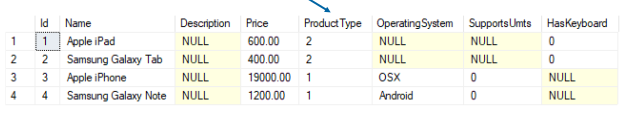
\includegraphics[width=0.8\linewidth]{images/table_per_hierarchy.png}
	\caption{Table per Hierarchy}
\end{figure}

\paragraph{Table per Type} Tabelle für jeden konkreten Typ mit allen benötigten Feldern. Keine Fremdschlüsselbeziehung (Parent-Child). Nachteil: Joins
\begin{itemize}
	\item \textbf{Tabelle ''Products''}: Id, Name, Description, Price
	\item \textbf{Tabelle ''MobilePhones''}: Id, OperatingSystem, SupportsUmts
	\item \textbf{Tabelle ''Tablets''}: Id, HasKeyboard
\end{itemize}

\paragraph{Table per concrete Type} Tabelle für Parent (gemeinsame Felder) und Tabellen für Childs (eigene Felder) mit Verweis auf Parent. Nachteil: Duplicate columns
\begin{itemize}
	\item \textbf{Tabelle ''Products''}: Id, Name, Description, Price
	\item \textbf{Tabelle ''MobilePhones''}: Id, Name, Description, Price, OperatingSystem, SupportsUmts
	\item \textbf{Tabelle ''Tablets''}: Id, Name, Description, Price, HasKeyboard
\end{itemize}

\subsection{Database Migration}
Während Entwicklung:
Modell anpassen, Migration erstellen, Review der Migration, eventuelle Korrekturen anbringen

Deployment:
Änderungen gemäss Migration-Reihenfolge auf Datenbank deployen, Rollback auf älteren Stand via Down-Migration möglich

\textbf{Migration erstellen}
\lstinline{dotnet ef migrations add InitialCreate}
-> DB wude noch nicht erstellt

\textbf{Datenbank Deployment}
\lstinline{dotnet ef database update}
-> DB wurde erstellt

\begin{lstlisting}
using(var context = new AngProjContext()) {
    var database = context.Database;
    //"Dev" Ansatz (loeschen / neu erstellen)
    database.EnsureDeleted(); //Loescht DB
    database.EnsureCreated(); //Erstellt DB falls nicht vorhanden
    
    //Automatische Migration auf neuesten Stand
    database.Migrate(); //Migration DB zur neusten Version
    
    //Migrations abfragen
    IEnumerable<string> migrations;
    migrations = database.GetMigrations(); //Abfrage von Migration-Names im DbContext
    migrations = database.GetPendingMigrations();
    migrations = database.GetAppliedMigrations();
    var m = context.GetService<IMigrator>(); 
    m.Migrate("<MigrationName>"); //Explizite Migration auf spezifische Version
}
\end{lstlisting}

\clearpage

\subsection{Data Type Mappings}
\begin{figure}[ht]
	\centering
	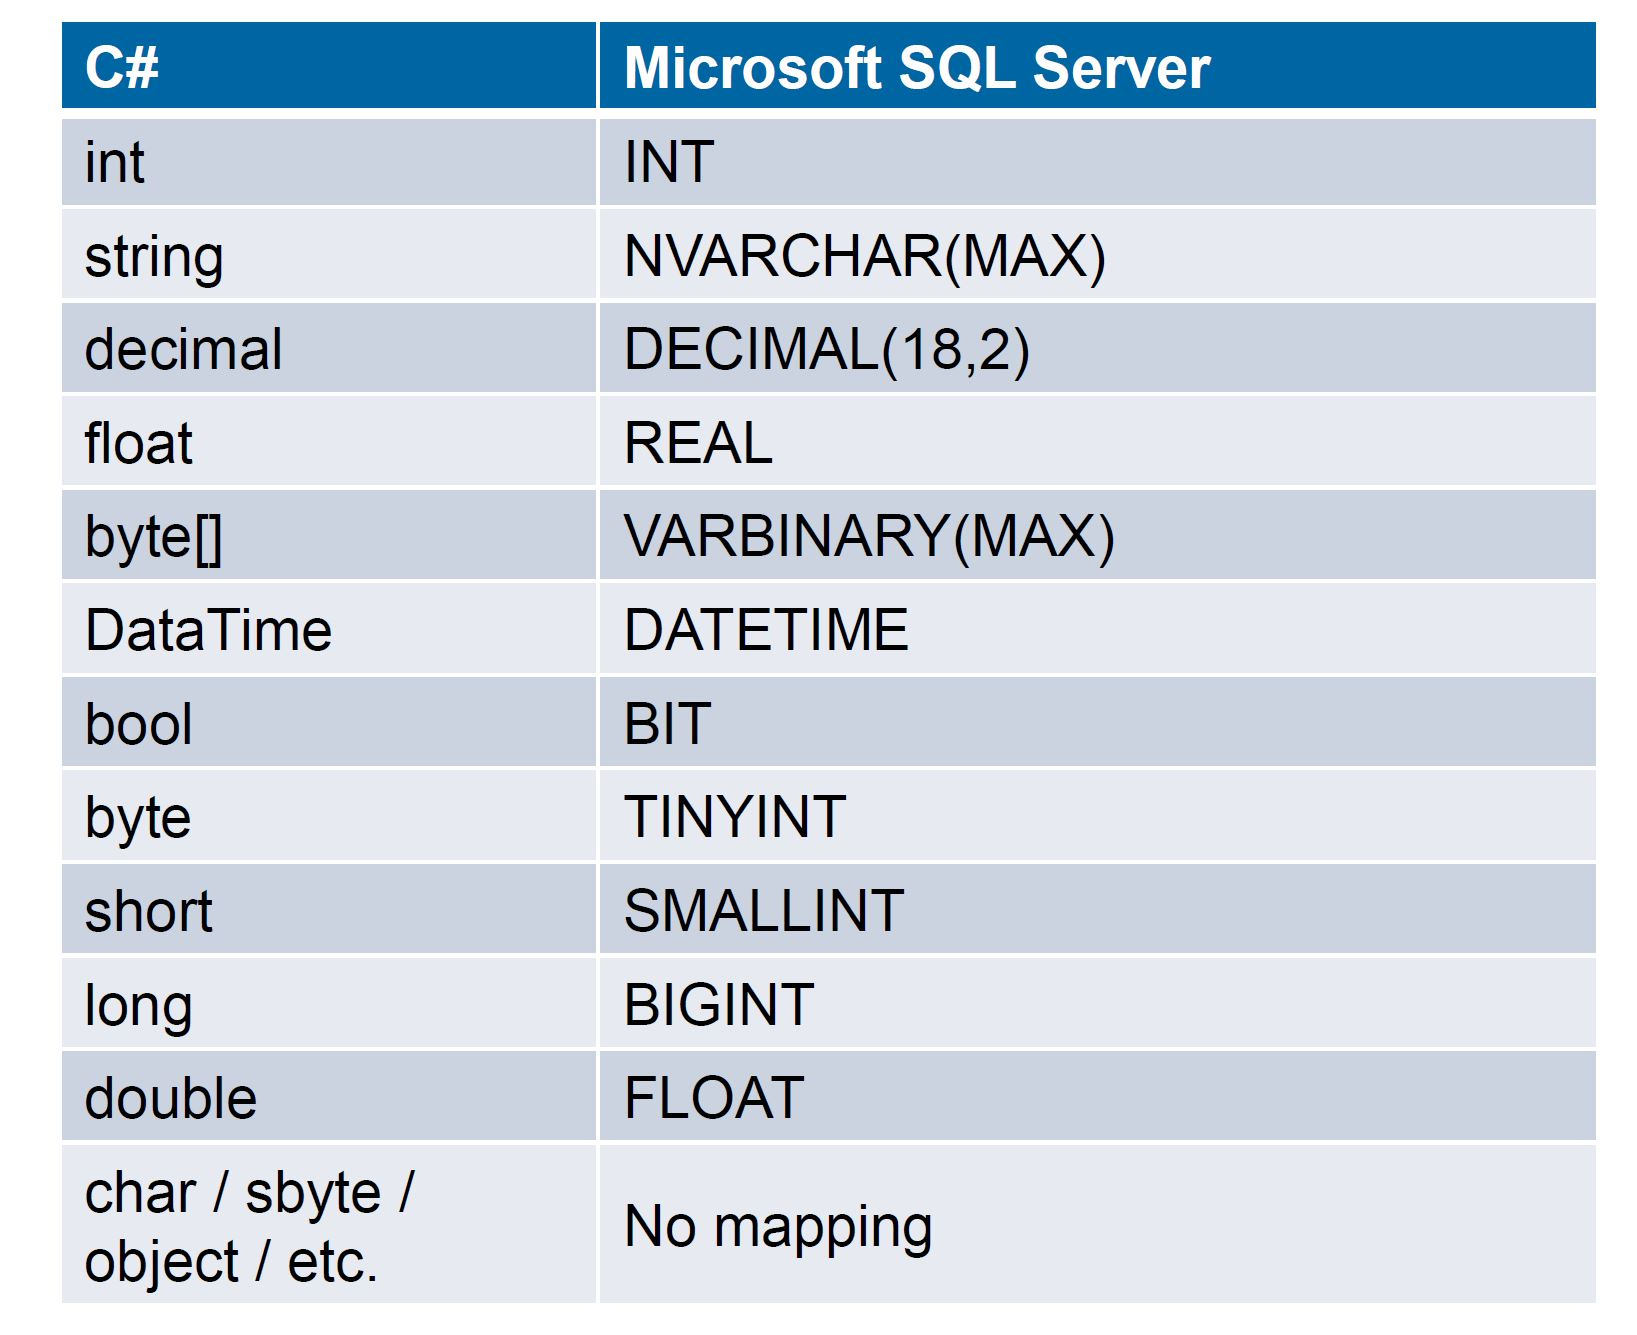
\includegraphics[width=0.7\linewidth]{images/datatypemappings}
	\caption{Data Type Mappings}
	\label{fig:datatypemappings}
\end{figure}

\section{GRPC: Google Remote Procedure Call}
Neue Standard-Technologie für Backend-Kommunikation in .NET Core. Hohe Performance von zentraler Bedeutung. gRPC ist ein Software Development Kit (SDK), Request-Response-orientiert, Plattform- und Sprach-neutral.
Kommunikation über HTTP/2 (Multiplexing (mehrere gRPC Calls pro TCP/IP Connection), Bidirectionales Streaming, Parallele Requests und Responses in einer einzigen TCP Verbindung, Kommunikation wegen HTTPS verschlüsselt).

\textbf{RPC} ermöglicht Client / Server Kommunikation und wird in fast allen verteilten Systemen verwendet.
\textbf{Grundprinzipien:} Einfache Service-Definition, Sprach-Unabhängigkeit, Problemlose Skalierbarkeit, Bi-direktionales Streaming, integrierte Authentisierungsmechanismen
\begin{figure}[!ht]
	\centering
	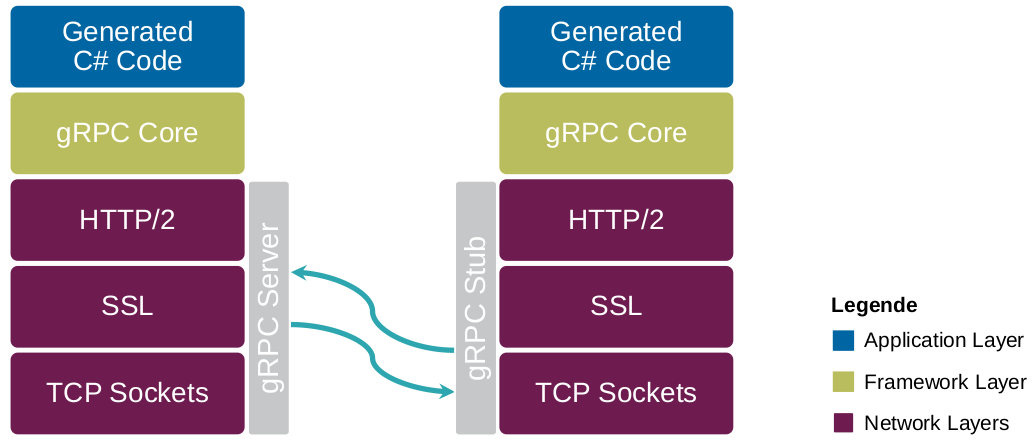
\includegraphics[width=0.6\linewidth]{images/grpc_architektur.png}
	\caption{gRPC Architektur}
	\label{fig:grpcarchitektur}
\end{figure}

\subsection{Protocol Buffers}
\begin{description}
	\item[Interface Definition Language (IDL)] Beschreibt ein Service Interface platform- und sprach-neutral.
	\item[Data Model] Beschreibt Messages resp. Request- und Response-Objekte.
	\item[Wire Format] Beschreibt das Binärformat zur Übertragung.
	\item[Serialisierungs-/Deserialisierungs-Machanismen]
	\item[Service-Versionierung]
\end{description}

\paragraph{Protocol Buffers / Fields / Scalar Value Types} .proto und C\#

\begin{minipage}[t]{0.9\textwidth}
	\centering
	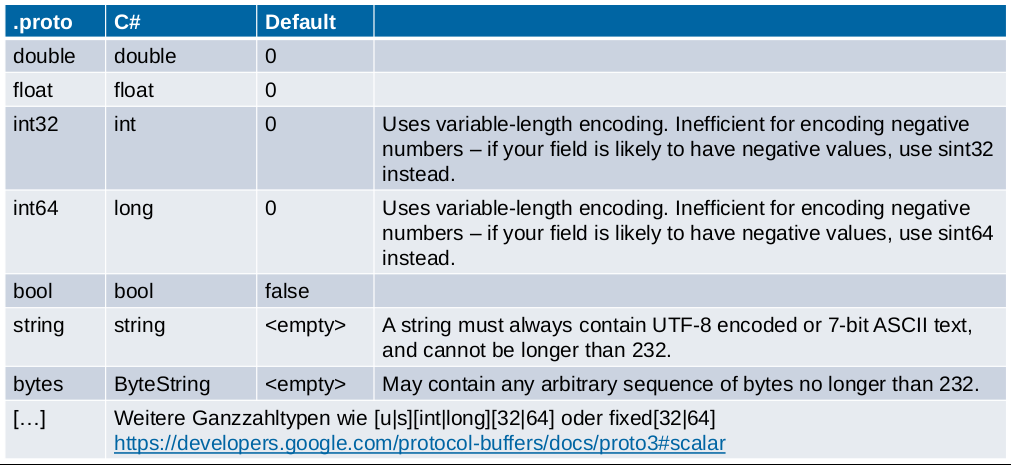
\includegraphics[width=0.9\linewidth]{images/grpc_buffers.png}
\end{minipage}

\paragraph{Proto Files} Datei-Endung *.proto, 1 oder mehr Services und mehrere Service-Methoden pro Service. 1 oder mehr Message Type Fields (Field definiert durch Type, Unique Name, Unique Field Number). Service-Methoden haben immer genau 1 Parameter und 1 Rückgabewert. Null-Werte mit \lstinline|google.protobuf.Empty|.
\begin{lstlisting}
syntax = "proto3";
option csharp_namespace = "_01_BasicExample";
package Greet;
service Greeter { //The greeting service definition
    rpc SayHello (HelloRequest) //sends a greeting
        returns (HelloReply);
    rpc GetAll(google.protobuf.Empty)               // Empty (Void) input
        returns (SearchDto);
    rpc Delete(SearchDto)
		returns (google.protobuf.Empty);            // Empty (Void) return
}
message HelloRequest { //The request message containing the user's name
    string name = 1;
}
message HelloReply { //The response message containing the greetings
    string message = 1;
}
\end{lstlisting}

\paragraph{Fields/Repeated Fields}
\begin{itemize}
	\item \textbf{Angabe des Feldtypen} Skalarer Werttyp, andere Message Type, Enumeration
	\item \textbf{Unique Field Name} Wird für Generatoren verwendet, Lower Snake Case (underscores)
	\item \textbf{Unique Field Number} Identifikator für das Binärformat.
\end{itemize}
\begin{lstlisting}
message SearchRequest {
    string query = 1;
    int32 page_number = 2;
    int32 result_per_page = 3;
}
message SearchResponse {
    repeated string results = 1;        // Repeated - Ergibt eine Liste von Strings
}
\end{lstlisting}

\paragraph{Enumerations} Definition innerhalb von Message oder Proto-File root, Enum-Member mit Wert 0 muss existieren (Default Value)
\begin{lstlisting}
message SearchRequest {
    Color searchColor = 1;
    Size searchSize = 2;
    enum Color {
        RED = 0; // 0 must exist
        GREEN = 1;
    }
}
enum Size {
    S = 0; // 0 must exist
    M = 1;
    L = 2;
}
\end{lstlisting}

\paragraph{Timestamp} \lstinline{Timestamp.FromDateTime(DateTime.UtcNow);}
\begin{lstlisting}
message TimestampResponse {
    repeated google.protobuf.Timestamp results = 1;
}
Timestamp von = Timestamp.FromDateTime(new DateTime(2021, 07, 15, 0, 0, 0, DateTimeKind.Utc));
\end{lstlisting}



\paragraph{Reserved keyword}
\begin{lstlisting}
message SearchRequest {
    reserved 1, 3, 20 to 30;
    reserved "page_number",
             "result_per_page";
             
    string query = 1; // Compilerfehler
    int32 page_number = 2; // Compilerfehler
    int32 result_per_page = 3; // Compilerfehler
}
\end{lstlisting}
\subsection{gRPC C\# API}
\paragraph{Protocol Buffers Compiler}
\begin{itemize}
	\item \textbf{protoc.exe mit Plugins für C\# Code Generierung}
	\item \textbf{Automatisch in Build Pipeline eingebunden}
	\item \textbf{NuGet Package} grpc.Tools
	\item \textbf{Proto-Compiler Output in ''obj'' Folder}
\end{itemize}

\paragraph{Aufbau Server Projekt} ASP.NET Core Projekt, erstellen via CLI (.net new grpc), NuGet Packages (Grpc.AspNetCore).
\begin{lstlisting}
// Server Projekt
<Project Sdk="Microsoft.NET.Sdk.Web">
    <ItemGroup>
        <Protobuf Include="Protos\greet.proto" GrpcServices="Server"> // zu generierende Klassen (Server)
            <Link>Protos\greet.proto</Link>         // File Link
        </Protobuf>
    </ItemGroup>
    <ItemGroup>
        <PackageReference Include="Grpc.AspNetCore" Version="..." />  // Packages
    </ItemGroup>
</Project>
\end{lstlisting}

\paragraph{Aufbau Client Projekt} Beliebiges Projekt, Proto-File als Kopie/Link eibinden, NuGet Packages (Grpc.Net.Client, Google.Protobuf, Grpc.Tools)
\begin{lstlisting}
// Client Projekt
<Project Sdk="Microsoft.NET.Sdk.Web">
    <ItemGroup>
        <Protobuf Include="..\<relative_path>\greet.proto" GrpcServices="Client"> // Protobuf Include (relativer Pfad) und zu generierende Klassen (Client)
            <Link>Protos\greet.proto</Link>
        </Protobuf>
    </ItemGroup>
    <ItemGroup>
        <PackageReference Include="Google.Protobuf" Version="..." />
        <PackageReference Include="Grpc.Net.Client" Version="..." />
        <PackageReference Include="Grpc.Tools" Version="...">[...]
        </PackageReference>
    </ItemGroup>
</Project>
\end{lstlisting}

\subsection{Beispiel Customer Service} 2 Services Customer Service und Order Service
\paragraph{Service/Proto-File}
\begin{lstlisting}
// Customer Service
service CustomerService {
    rpc GetCustomers (google.protobuf.Empty) //Liste aller Kunden
        returns (GetCustomersResponse);
    rpc GetOrders (GetOrdersRequest) //einzelner Kunde 
        returns (GetOrdersResponse);
}

// Order Service
service OrderService {
    rpc GetCustomer (GetCustomerRequest) //Alle Bestellungen zu einem Kunden
        returns (GetCustomerResponse);
}
\end{lstlisting}

\paragraph{Messages/Proto-File}
\begin{lstlisting}
// Customer Messages
message GetCustomersResponse {
    repeated CustomerResponse data = 1;
}
message GetCustomerResponse {
    CustomerResponse data = 1;
}
message GetCustomerRequest {
    int32 id_filter = 1;
    bool include_orders = 2;
}
message CustomerResponse {
    int32 id = 1;
    string first_name = 2;
    string last_name = 3;
    Gender gender = 4;
    repeated OrderResponse orders = 10;
}
enum Gender { UNKNOWN = 0; FEMALE = 1; MALE = 2; }

// Order Messages
message GetOrdersRequest {
    int32 customer_id_filter = 1;
}
message GetOrdersResponse {
    repeated OrderResponse data = 1;
}
message OrderResponse {
    string product_name = 1;
    int32 quantity = 2;
    double price = 3;
}
\end{lstlisting}

\paragraph{Service Implementation}
\begin{lstlisting}
//Customer Service
public class MyCustomerService : CustomerService.CustomerServiceBase {
    public override async Task<GetCustomersResponse> GetCustomers(Empty request, ServerCallContext context) { /* ... */ }
    public override async Task<GetCustomerResponse> GetCustomer(GetCustomerRequest request, ServerCallContext context) { /* ... */ }
}

//Order Service
public class MyOrderService : OrderService.OrderServiceBase {
    public override async Task<GetOrdersResponse> GetOrders(GetOrdersRequest request, ServerCallContext context) { /* ... */ }
}
\end{lstlisting}

\paragraph{Client-Implementation (Customer)}
\begin{lstlisting}
// The port number (5001) must match the port of the gRPC server.
GrpcChannel channel = GrpcChannel.ForAddress("https://localhost:5001");
// Customer service calls
var customerClient = new CustomerService.CustomerServiceClient(channel);
var request1 = new Empty();
GetCustomersResponse response1 = await customerClient.GetCustomersAsync(request1);
Console.WriteLine(response1);
var request2 = new GetCustomerRequest { IdFilter = 1 };
GetCustomerResponse response2 = await customerClient.GetCustomerAsync(request2);
Console.WriteLine(response2);
request2.IncludeOrders = false;
response2 = await customerClient.GetCustomerAsync(request2);
Console.WriteLine(response2);
\end{lstlisting}

\paragraph{Client-Implementation (Order)}
\begin{lstlisting}
// The port number (5001) must match the port of the gRPC server.
GrpcChannel channel = GrpcChannel.ForAddress("https://localhost:5001");
// Order service calls
var orderClient = new OrderService.OrderServiceClient(channel);
var request3 = new GetOrdersRequest { CustomerIdFilter = 1 };
GetOrdersResponse response3 = await orderClient.GetOrdersAsync(request3);
Console.WriteLine(response3);
\end{lstlisting}

\subsection{Streams}
\begin{description}
	\item[Unterstützt 3 Modi] Server Streaming Call (Server > Client), Client Streaming Call (Client > Server), Bidirectional/Duplex Streaming Call. Schlüsselwort ''stream'' vor Typenbezeichnung.
	\item[Reliability] End-to-End Reliability (garantiertes Ausliefern der Nachrichten gewährleistet), Ordered Delivery (Reihenfolge gewährleistet)
\end{description}
\begin{lstlisting}
service FileStreamingService {
    rpc ReadFiles (google.protobuf.Empty) //Server Streaming Call
        returns (stream FileDto);
    rpc SendFiles (stream FileDto) //Client Streaming Call
        returns (google.protobuf.Empty);
    rpc RoundtripFiles (stream FileDto) //Bi-directional / Duplex Streaming Call
        returns (stream FileDto);
}
message FileDto {
    string file_name = 1;
    int32 line = 2;
    string content = 3;
}
\end{lstlisting}

\paragraph{Server Streaming Call (Server > Client) Service}
\begin{lstlisting}
//Client
using (AsyncServerStreamingCall<FileDto> call = client.ReadFiles(new Empty())) {
    await foreach (FileDto message in call.ResponseStream.ReadAllAsync()) { // Read last written chunk
        WriteLine($"File: {message.FileName}, Line Nr: {message.Line}, Line Content: {message.Content}");
    }
}

//Service
public override async Task ReadFiles(Empty request, IServerStreamWriter<FileDto> responseStream, ServerCallContext context) {
    string[] files = Directory.GetFiles(@"...");
    foreach (string file in files) {                // Files Loop
        string content; int line = 0;
        using StreamReader reader = File.OpenText(file);
        while ((content = await reader.ReadLineAsync()) != null) {      // Line-Loop
            line++;
            FileDto reply = new FileDto {
                FileName = file, Line = line, Content = content,
            };
            await responseStream.WriteAsync(reply); // Write to Stream
        }
    }
}
\end{lstlisting}

\paragraph{Client Streaming Call (Client > Server) Service}
\begin{lstlisting}
//Service
public override async Task<Empty> SendFiles(IAsyncStreamReader<FileDto> requestStream, ServerCallContext context) {    // Request Stream
    await foreach (FileDto message in requestStream.ReadAllAsync()) {   // Read last written chunk
        WriteLine($"File: {message.FileName}, Line Nr: {message.Line}, Line Content: {message.Content}");
    }
    return new Empty();     // Empty Result
}

//Client
using (AsyncClientStreamingCall<FileDto, Empty> call = client.SendFiles()) {
    string[] files = Directory.GetFiles(@"Files");
    foreach (string file in files) { //File-Loop
        string content; int line = 0;
        using StreamReader reader = File.OpenText(file);
        while ((content = await reader.ReadLineAsync()) != null) { // Line-Loop
            line++;
            FileDto reply = new FileDto {
                FileName = file, Line = line, Content = content,
            };
            await call.RequestStream.WriteAsync(reply); // Write to Stream
        }
    }
    // Required!
    await call.RequestStream.CompleteAsync(); // Close Stream
    await call; // Wait until all requests are submitted
}
\end{lstlisting}

\paragraph{Bi-directional (Client > Server) Client}
\begin{lstlisting}
//Service
public override async Task RoundtripFiles(IAsyncStreamReader<FileDto> requestStream, IServerStreamWriter<FileDto> responseStream, ServerCallContext context) {
    await foreach (FileDto message in requestStream.ReadAllAsync()) { // Read last written chunk
        await responseStream.WriteAsync(message); // Write to Stream
        WriteLine($"File: {message.FileName}, Line Nr: {message.Line}, Line Content: {message.Content}");
    }
}

//Client
using (AsyncDuplexStreamingCall<FileDto, FileDto> call = client.RoundtripFiles()) {
    // Read
    Task readTask = Task.Run(async () => { // Read Task (no await)
        await foreach (FileDto message in call.ResponseStream.ReadAllAsync()) { // Read last written chunk
            WriteLine($"File: {message.FileName}, Line Nr: {message.Line}, Line Content: {message.Content}");
        }
    });
    
    // Write
    string[] files = Directory.GetFiles(@"Files");
    foreach (string file in files) {    // File-Loop
        string content; int line = 0;
        using StreamReader reader = File.OpenText(file);
        while ((content = await reader.ReadLineAsync()) != null) { // Line-Loop
            line++;
            FileDto reply = new FileDto {
                FileName = file, Line = line, Content = content,
            };
            await call.RequestStream.WriteAsync(reply); // Write to Stream
        }
    }
    await call.RequestStream.CompleteAsync();   // Close Stream
    await readTask; // Wait until all requests are submitted
}
\end{lstlisting}

\subsection{Special Types}
\paragraph{Timestamp} UTC Zeitstempel - muss UTC sein, es darf nicht DateTime.Now verwendet werden. \lstinline{Timestamp ts = Timestamp.FromDateTime(DateTime.UtcNow}
\paragraph{Collections - Map Fields} Generiert ein Map Field Property, ist read only
\begin{lstlisting}
message MapResonse { map<int32, string> string results = 1; }
var response = new MapResponse();
response.Results.Add(1, "Hello");
response.Results.ContainsKey(1);    response.Results[1];
\end{lstlisting}
\paragraph{Oneof} - Lässt eine Auswahl von Typen zu
\begin{lstlisting}
message OneofResponse {
    oneof results {
        string image_url = 1;
        bytes image_data = 2;
    }
}
\end{lstlisting}
\paragraph{Any} - Repräsentiert einen beliebigen Wert\lstinline{google.protobuf.Any results = 1;}

\subsection{Exception Handling}
Grundsätzlich immer via ''RpcException'' (basierend auf StatusCodes).
\begin{lstlisting}
public class RpcException : Exception {
    public RpcException(Status status);
    public RpcException(Status status, string message);
    public RpcException(Status status, Metadata trailers);
    public RpcException(Status status, Metadata trailers, string message);
    public Status Status { get; }
    public StatusCode StatusCode { get; }
    public Metadata Trailers { get; }
}
\end{lstlisting}
\paragraph{Status Codes} \hfill
\begin{figure}[!ht]
	\centering
	\begin{minipage}{.5\textwidth}
		\centering
		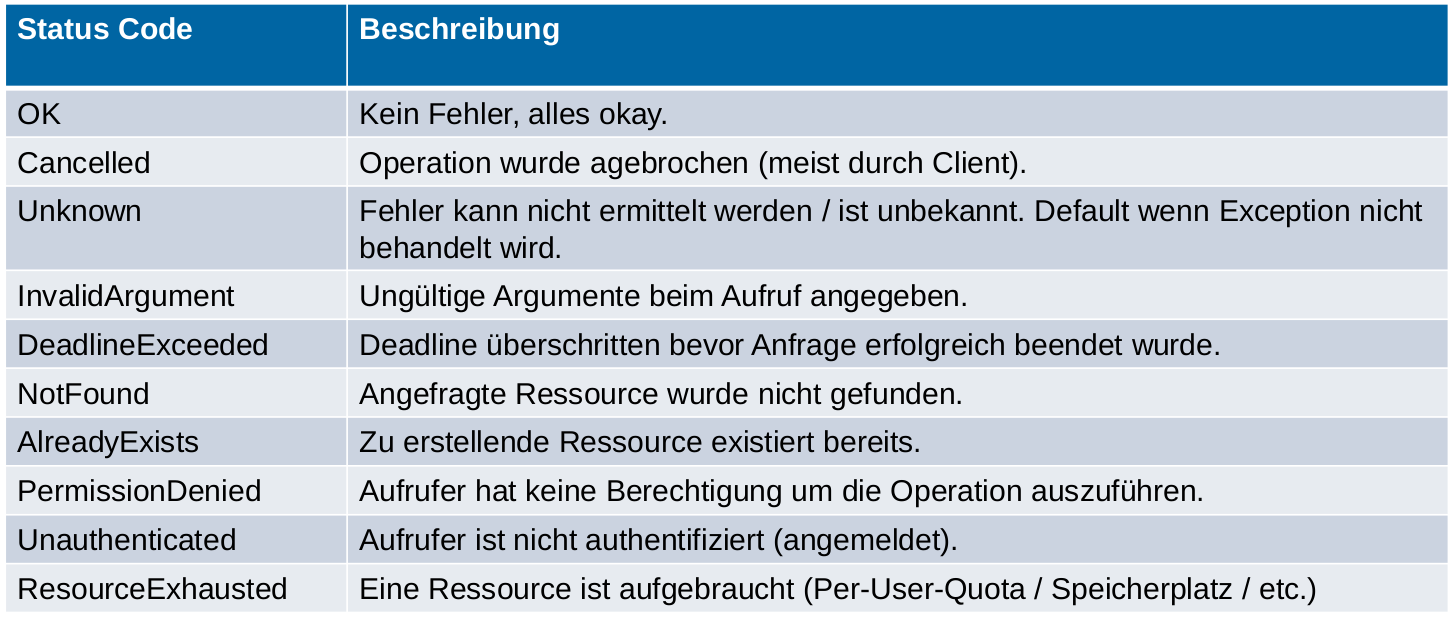
\includegraphics[width=0.49\linewidth]{images/grpc_status_codes_1.png}
		\caption{$dt=0.1$}
	\end{minipage}%
	\begin{minipage}{0.5\textwidth}
		\centering
		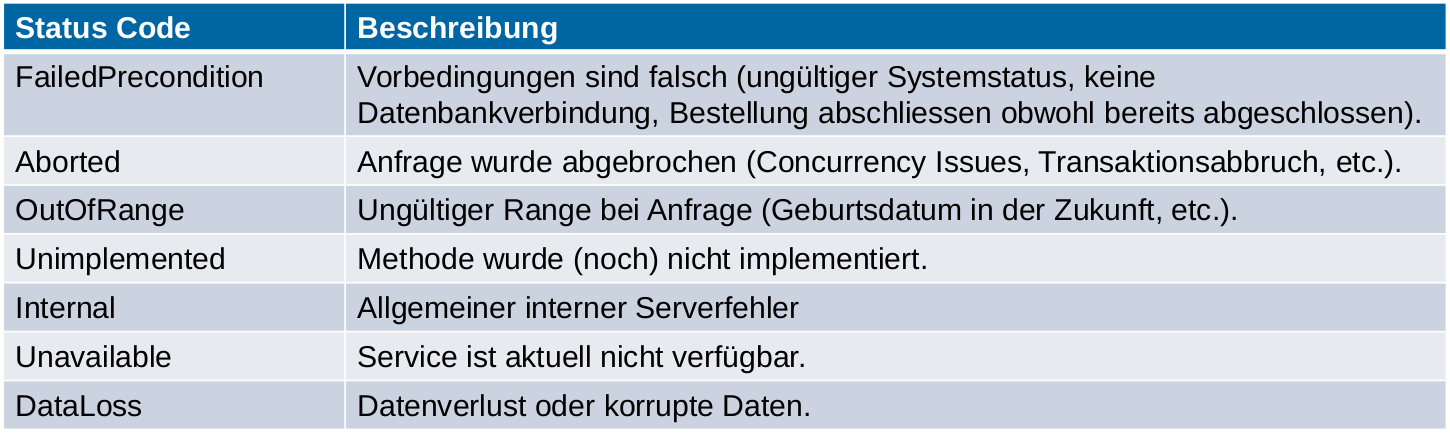
\includegraphics[width=0.49\linewidth]{images/grpc_status_codes_2.png}
		\caption{$dt =$}
	\end{minipage}
\end{figure}


\paragraph{Unbehandelte Exception} Exception wird auf Server nicht gefangen (Server Runtime fängt Exception, Wirft RpcException)
\begin{lstlisting}
public override async Task<Empty> Unhandled(Empty request, ServerCallContext context) {
    throw new Exception("Unhandled Exception");
}
\end{lstlisting}

\paragraph{Behandelte Exception mit Trailers} Exception wird auf Server gefangen und korrekt verpackt. Metadata-Klassen verwenden, Key-Value-Pair-Liste.
\begin{lstlisting}
public override async Task<Empty> Trailers(Empty request, ServerCallContext context) {
    throw new RpcException(new Status(StatusCode.NotFound, "Something was not found."),
        new Metadata {
            { "error-details", "Here are some more details..." },
            { "error-obj" + Metadata.BinaryHeaderSuffix, Encoding.UTF8.GetBytes("...payload...") }
        }
    );
}
\end{lstlisting}

\section{Reflection}

\begin{figure}[!ht]
	\centering
	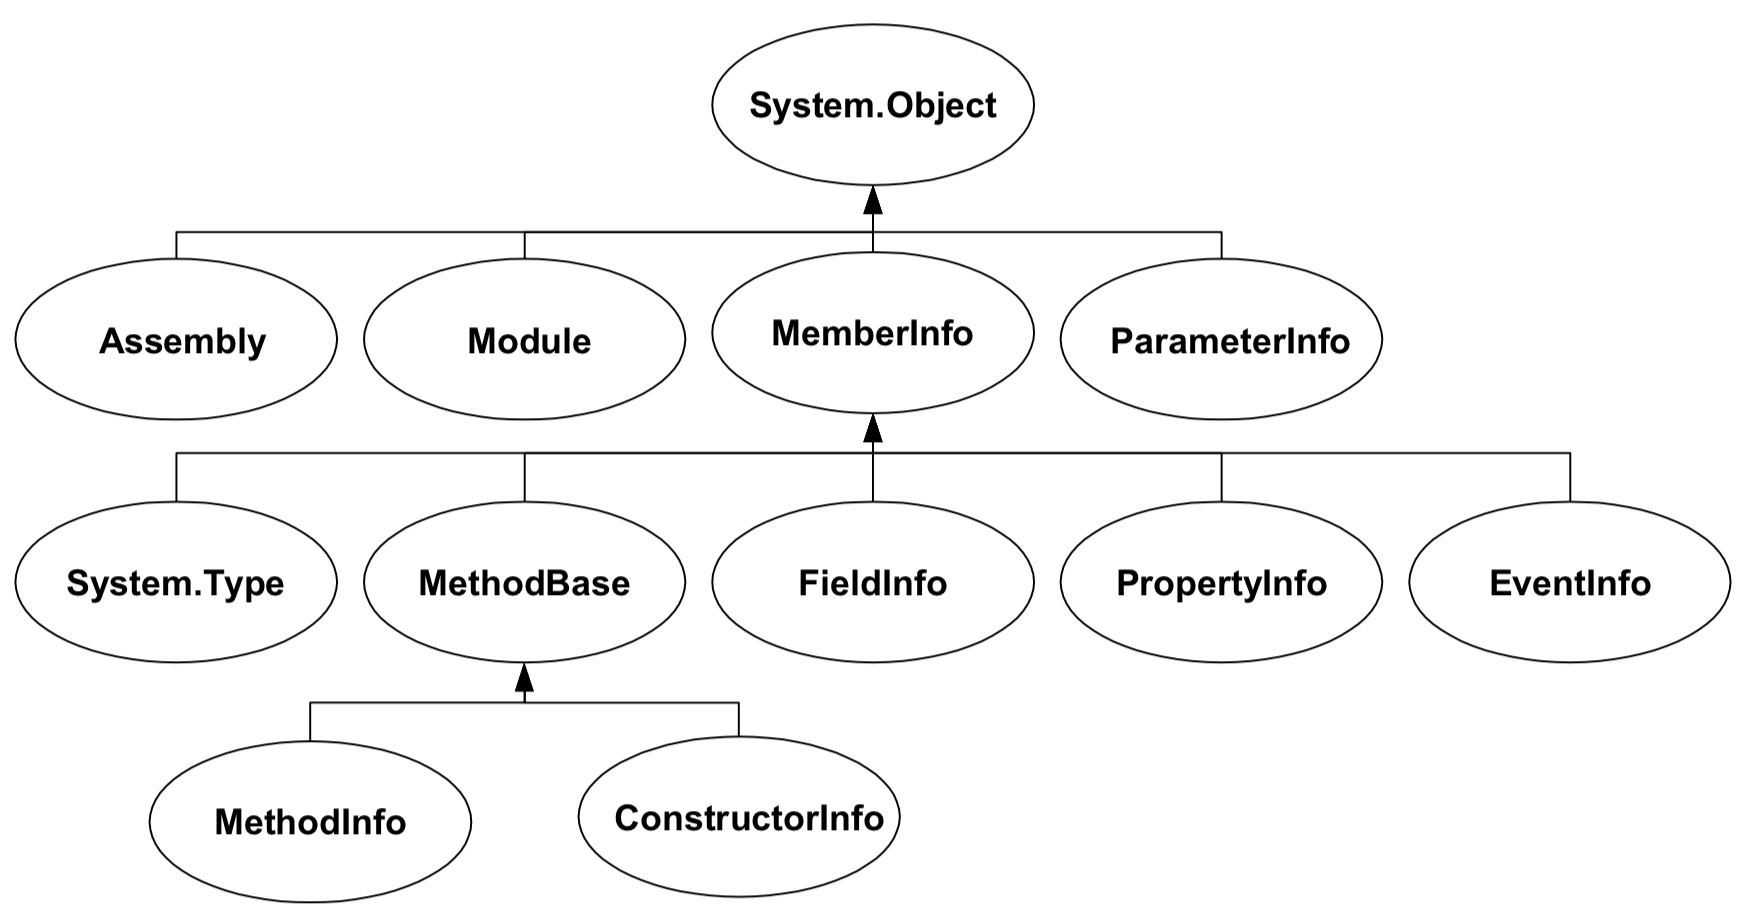
\includegraphics[width=0.8\linewidth]{images/member_hierarchie}
	\caption{Typ-Hierarchie}
	\label{fig:valuetypes}
\end{figure}

\subsection{Anwendungen}
\begin{description}
	\item[Metadaten erstellen] Darstellung der Metadaten in Tools
	\item[Type Discovery] Suchen und Instanzieren von Typen, Zugriff auf dynamische Datenstrukturen.
	\item[Late Binding (Methods/Properties] Aufruf von Methoden / Properties nach Type Discovery
	\item[Reflection Emit / Code-Emittierung] Erstellen von Typen inkl. Members zur Laufzeit
	\item[Alle Typen in der Common Language Runtime (CLR) sind selbst-definierend]
	\item[Nicht zugreifbare Members auch einsehbar] z.b. private Felder
	\item[Klasse ''System.Type''] Einstiegspunkt aller Reflection-Operationen, repraesentiert einen Typen mit all seinen Eigenschaften, abstrakte Basisklasse, ''Sysemt.RuntimeType'' wird jeweils verwendet.
	\item[Ermitteln von ''System.Type'' via] \lstinline|"obj".GetType()|, \lstinline|typeof("classname")|.
\end{description}
\begin{lstlisting}
this.GetType() // implemented on object
typeof(MyClass) || typeof(int)
\end{lstlisting}

\subsection{Type Discovery}
Suche alle Typen in einem Assembly.
\begin{lstlisting}[caption=Reflection: Type Discovery]
Assembly a01 = Assembly.Load("mscorlib, PublicKeyToken=b77a5c561934e089, Culture=neutral, Version=4.0.0.0");
// Assembly.Load("File.dll") File auslesen
Type[] t01 = a01.GetTypes();
foreach (Type type in t01) {
	Console.WriteLine(type);
	MemberInfo[] mInfos = type.GetMembers();
	foreach (var mi in mInfos) 	{
		Console.WriteLine(
		"\t{0}\t{1}",
		mi.MemberType,
		mi);
	}
}
\end{lstlisting}


\subsection{Member auslesen}
Das Auslesen von Members kann mit \lstinline|BindingFlags| gefiltert werden.
\begin{lstlisting}[caption=Reflection: Members auslesen]
Type type = typeof(Counter);
MemberInfo[] miAll = type.GetMembers();
foreach (MemberInfo mi in miAll) {
	Console.WriteLine("{0} is a {1}", mi, mi.MemberType);
}
Console.WriteLine("----------");
PropertyInfo[] piAll = type.GetProperties();
foreach (PropertyInfo pi in piAll) {
	Console.WriteLine("{0} is a {1}",	pi, pi.PropertyType);
}

// ex2: filter members according to BindingFlag or Filtername
Type type = typeof(Assembly);
BindingFlags bf =
	BindingFlags.Public |
	BindingFlags.Static |
	BindingFlags.NonPublic |
	BindingFlags.Instance |
	BindingFlags.DeclaredOnly;

System.Reflection.MemberInfo[] miFound = type.FindMembers(
	MemberTypes.Method, bf, Type.FilterName, "Get*"
);
\end{lstlisting}

\subsection{Field Information}
Die Field Info beschreibt ein Feld einer Klasse (Name, Typ, Sichtbarkeit). Die Felder können mit \lstinline|object GetValue(object obj)| und \lstinline|void SetValue(object obj, object value)| auch gelesen und geschrieben werden.

\begin{lstlisting}[caption=Reflection: Field Info]
Type type = typeof (Counter);
Counter c = new Counter(1);

// All Fields
FieldInfo[] fiAll = type.GetFields(BindingFlags.Instance | BindingFlags.NonPublic);
	
// Specific Field
FieldInfo fi = type.GetField("countValue", BindingFlags.Instance | 	BindingFlags.NonPublic);
	
int val01 = (int) fi.GetValue(c);
c.Increment();
int val02 = (int) fi.GetValue(c);
fi.SetValue(c, -999);
\end{lstlisting}


\subsection{Property Information}
Die Property Info beschreibt eine Property einer Klasse (Name, Typ, Sichbarkeit, Informationen zu Get/Set). Auch Properties lassen sich lesen und schreiben.
\begin{lstlisting}[caption=Reflection: Property Info]
Type type = typeof(Counter);
Counter c = new Counter(1);

// All Properties
PropertyInfo[] piAll = type.GetProperties();

// Specific Property
PropertyInfo pi = type.GetProperty("CountValue");

int val01 = (int)pi.GetValue(c);
c.Increment();
int val02 = (int)pi.GetValue(c);
if(pi.canWirte) { pi.SetValue(c, -999); }
\end{lstlisting}

\subsection{Method Info}
Die Method Info beschreibt eine Methode einer Klasse (Name, Parameter, Rückgabewert, Sichtbarkeit). Sie leitet von Klasse \lstinline|MethodBase| ab. Die Methode wird mit \lstinline|Invoke()| aufgerufen.
\begin{lstlisting}[caption=Reflection: Method Info]
Type type = typeof(Counter);
Counter c = new Counter(1);

// All Methods
MethodInfo[] miAll = type.GetMethods();

// Specific Method
MethodInfo mi = type.GetMethod("Increment");
mi.Invoke(c, null);
\end{lstlisting}

\subsection{Constructor Info}
Die Constructor Info beschreibt ein Konstruktor einer Klasse (Name, Parameter, Sichtbarkeit). Wie Method Info leitet er wegen seinen ähnlichen Eigenschaften von \lstinline|MethodBase| ab und wird  mit \lstinline|Invoke()| aufgerufen.
\begin{lstlisting}[caption=Reflection: Constructor Info]
Type type = typeof(Counter);
Counter c = new Counter(1);

// All Constructors
var ciAll = type.GetConstructors();

// Specific Constructor Overload 01
ConstructorInfo ci01 = type.GetConstructor(new[] { typeof(int) });
Counter c01 = (Counter)ci01.Invoke(new object[] { 12 });

// Specific Constructor Overload 02
ConstructorInfo ci02 = type.GetConstructor(BindingFlags.Instance|BindingFlags.NonPublic, null, new Type[0], null);
Counter c02 = (Counter)ci02.Invoke(null);
\end{lstlisting}


\subsection{Example of Reflection Usage}
\begin{lstlisting}
using System.Reflection;

namespace TestReflection {
    class Program {
        static void Main(string[] args)  {
            var ass=Assembly.LoadFrom("Autos.dll");
            var t = ass.GetType("Autos.FastCars");
            var c=Activator.CreateInstance(t, new object[] {"Lamborghini"});
            var m = t.GetMethod("AutoFahren");
            m.Invoke(c, new object[]{});
        }
    }
} 
\end{lstlisting}

\subsection{Attributes}
\begin{lstlisting}[caption=Reflection: Attributes]
Type type = typeof(MyMath);

// All Class Attributes
object[] aiAll = type.GetCustomAttributes(true);

// Check Definition
bool aiDef = type.IsDefined(typeof(BugfixAttribute));
\end{lstlisting}

\section{Attributes}
Attributes sind das C\# Pendant zu den Java Annotations. Bei Attributen geht es um die aspektorientierte Programmierung. z.B Erweiterung eines Attributes um eine Aspekt Serialisierung, Transactions, etc. Es können auch eigene Attribute geschrieben werden. Diese leiten immer von \lstinline|System.Attribute| ab. Attribute können mit über Reflection abgefragt werden.
\begin{lstlisting}[caption=Attributes]
[DataContract, Serializable]
[Obsolete]
// Etc.
public class Auto {
	[DataMember]
	public string Marke { get; set; }
	[DataMember]
	public string Typ { get; set; }
}

// Beliebig viele Attribute
[DataContract][Serializabel] <=> [DataContract, Serializabel]

// Parameter
[DataContract] // Ohne Parameter
[DataContract(Name="MyParam")] // Named Parameter
[Obsolete("Alt!",  true)] // Positional Parameter
[Obsolete("Alt!", IsError=true)] // Mixed
\end{lstlisting}

\subsection{Anwendungsfälle}
\begin{itemize}
	\item Object-relationales Mapping
	\item Serialisierung (WCF, XML)
	\item Security und Zugriffsteuerung
	\item Dokumentation
\end{itemize}

\subsection{Typen}
Man unterscheidet zwei Typen von Attributen
\begin{enumerate}
	\item Intrinsic Attributes: Kommen bereits mit der \gls{clr} mit
	\item Custom Atttributes: Eigens definierte Attributre
\end{enumerate}

\clearpage

\subsection{Eigene Attribute}
Bei der Deklaration können die Objekte eingegrenzt werden, auf die das Attribute angewendet werden kann. Jedes Attribute muss als Postfix ''Attribute'' haben. (xxAttribute). Beim Verwenden wird der Postfix jedoch weggelassen.
\begin{lstlisting}
// declaration 
[AttributeUsage(                    //definiert wo attribute verwendet werden duerfen
	AttributeTargets.Class |
	AttributeTargets.Constructor |
	AttributeTargets.Field |
	AttributeTargets.Method |
	AttributeTargets.Property,
	AllowMultiple = true)]
public class BugfixAttribute : Attribute
{
	public BugfixAttribute(int bugId, string programmer, string date) {..}
	public int BugId { get; }
	public string Date { get; }
	public string Programmer { get; }
	public string Comment { get; set; }
}

// usage
[Bugfix(121, "MichaelWieland", "14/12/16")]
\end{lstlisting}
\paragraph{CSV-Filter}
\begin{lstlisting}
// list
var a = new List<Address> {
	new Address("Hans", "Strasse 16", "8645", "Jona") ,
	new Address("Hans2", "Strasse 2", "8645", "Jona")
}
Writer.SaveToCsv(a, @"C:\Temp\test.csv");

// address
public class Address {
	[CsvName("Name"), Uppercase]
	public string Name { get; set; }
	[CsvName("Strasse"), Lowercase]
	public string Street { get; set; }
	[CsvName("Plz")]
	public string Postcode { get; set; }
	...
}

// Custom Attributes
public class CsvNameAttribute : Attribute {     // Mapping eines Properties auf CSV Spalte
	public string Name { get; set; }
	public CsvAttribute(string name) {
		Name = name;
	}
}

public interface IStringFilter {            // beschreibt beliebigen Filter
	string Filter(string arg); 
}
public class UppercaseAttribute : Attribute : IStringFilter {       // Implementation von IStringFilter
	public string Filter(string arg) {
		return arg.ToUpper();
	}
}
public class LowercaseAttribute : Attribute : IStringFilter {       // Implementation von IStringFilter
	public string Filter(string arg) {
		return arg.ToLower();
	}
}
\end{lstlisting}

\subsection{Reflection Emit}
Reflection.Emit erlaubt neue Assemblies und Typen zur Laufzeit zu erzeugen und sofort zu verwnden. Erzeugen von Assemblies, neuen Modulen, neuen Typen, symbolischer Metainformationen für bestehende Module.
\paragraph{Wichtigste Klassen}
\begin{itemize}
	\item AssemblyBuilder $\Rightarrow$ Assemblies definieren
	\item ModuleBuilder $\Rightarrow$ Module definieren
	\item TypeBuilder $\Rightarrow$ Typen definieren
	\item MethodBuilder $\Rightarrow$ Methoden definieren
	\item ILGenerator $\Rightarrow$ IL-Code erzeugen
\end{itemize}

\paragraph{Assembly inkl. Module definieren}\mbox{} \\
\begin{lstlisting}
AssemblyName assemblyName = new AssemblyName("Hsr.EmitDemoAssembly");
AssemblyBuilder assemblyBuilder = AppDomain.CurrentDomain.DefineDynamicAssembly(assemblyName, AssemblyBuilderAccess.RunAndSave);
ModuleBuilder moduleBuilder = assemblyBuilder.DefineDynamicModule("Hsr.EmitDemoModule", "Hsr.EmitDemoAssembly.dll");
\end{lstlisting}

\paragraph{Klasse ''EmitDemo'' definieren}\mbox{} \\
\begin{lstlisting}
TypeBuilder typeBuilder = moduleBuilder.DefineType("EmitDemo", TypeAttributes.Public);
\end{lstlisting}

\paragraph{Methode ''SayHello'' definieren}\mbox{} \\
\begin{lstlisting}
Type[] paramTypes = { typeof(string) };
Type retType = typeof(string);
MethodBuilder methodBuilder = typeBuilder.DefineMethod("SayHelloTo",
        MethodAttributes.Public | MethodAttributes.Virtual, retType, paramTypes);
\end{lstlisting}

\paragraph{Einfügen der MSIL Operationen in die neu erzeugte Methode}\mbox{} \\
\begin{lstlisting}
ILGenerator ilGen = methodBuilder.GetILGenerator();
ilGen.Emit(OpCodes.Ldstr, "Hello ");
ilGen.Emit(OpCodes.Ldarg_1);
MethodInfo mi = typeof(string).GetMethod("Concat", new[] { typeof(string), typeof(string) });
ilGen.Emit(OpCodes.Call, mi);
ilGen.Emit(OpCodes.Ret);
\end{lstlisting}

\paragraph{Klasse ''EmitDemo'' erzeugen}\mbox{} \\
\begin{lstlisting}
typeBuilder.CreateType();
\end{lstlisting}

\paragraph{Methode ''SayHello'' ausführen}\mbox{} \\
\begin{lstlisting}
MethodInfo method = typeBuilder.GetMethod("SayHelloTo", new[] { typeof(string) });
object obj = Activator.CreateInstance(typeBuilder);
object ret = method.Invoke(obj, new object[] { "HSR" });
Console.WriteLine(ret);
\end{lstlisting}

\paragraph{Assembly ''Hsr.EmitDemoAssembly.dll'' abspeichern}\mbox{} \\
\begin{lstlisting}
assemblyBuilder.Save(assemblyName.Name + ".dll");
\end{lstlisting}


% \section{Reflection}
% Unter Reflection versteht man die Analyse von Metadaten eines Objekts zur Laufzeit. Mit Reflection lassen sich Typen suchen und instanzieren. Die abstrakte Basisklasse \lstinline|System.Type| representiert einen Typen. \lstinline|System.RuntimeType| erbt von \lstinline|System.Type|. Mit Reflection können auch \lstinline|private| Felder gelesen und geschreiben werden.

% \begin{figure}[!ht]
% \centering
% 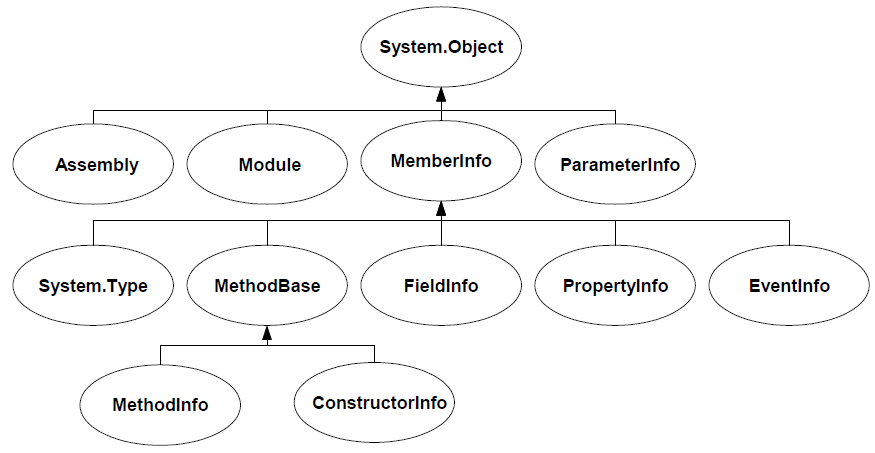
\includegraphics[width=0.8\linewidth]{images/reflection-type-hiearchy}
% \caption{Reflection Type-Hierarchy}
% \label{fig:mex}
% \end{figure}

% \begin{figure}[!ht]
% \centering
% 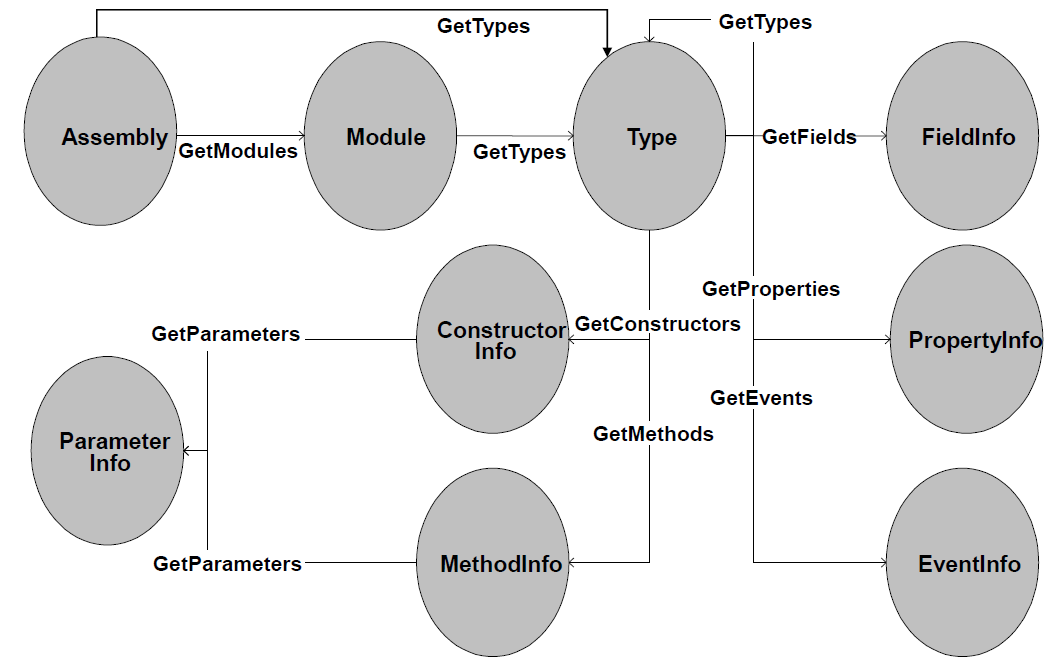
\includegraphics[width=0.8\linewidth]{images/reflection-navigation}
% \caption{Reflection Navigation}
% \label{fig:mex}
% \end{figure}

% \begin{lstlisting}[caption=Reflection]
% this.GetType() // implemented on object
% typeof(MyClass) || typeof(int)
% \end{lstlisting}

% \subsection{Type Discovery}
% Suche alle Typen in einem Assembly.
% \begin{lstlisting}[caption=Reflection: Type Discovery]
% Assembly a01 = Assembly.Load("mscorlib, PublicKeyToken=b77a5c561934e089, Culture=neutral, Version=4.0.0.0");
% Type[] t01 = a01.GetTypes();
% foreach (Type type in t01)
% {
% 	Console.WriteLine(type);
% 	MemberInfo[] mInfos = type.GetMembers();
% 	foreach (var mi in mInfos)
% 	{
% 		Console.WriteLine(
% 		"\t{0}\t{1}",
% 		mi.MemberType,
% 		mi);
% 	}
% }

% // Output
% ...
% System.Int32
%     Method Int32 CompareTo(System.Object)
%     Method Int32 CompareTo(Int32)
%     Method Boolean Equals(System.Object)
%     Method Boolean Equals (Int32)
%     ...
%     Method System.String ToString()
% ...
% \end{lstlisting}


% \subsection{Member auslesen}
% Das Auslesen von Members kann mit \lstinline|BindingFlags| gefiltert werden.
% \begin{lstlisting}[caption=Reflection: Members auslesen]
% Type type = typeof(Counter);
% MemberInfo[] miAll = type.GetMembers(); // Methods & Properties
% foreach (MemberInfo mi in miAll) {
% 	Console.WriteLine("{0} is a {1}", mi, mi.MemberType);
% }
% Console.WriteLine("----------");
% PropertyInfo[] piAll = type.GetProperties();
% foreach (PropertyInfo pi in piAll) {
% 	Console.WriteLine("{0} is a {1}",	pi, pi.PropertyType);
% }

% // Output:
% ...
% Int32  get_CountValue()  is  a  Method 
% Void  set_CountValue(Int32)  is  a  Method 
% Void Increment() is a Method
% Void Decrement() is a Method 
% String  ToString()  is  a  Method 
% Boolean Equals(Object) is a Method 
% Int32  GetHashCode()  is  a  Method 
% Type  GetType()  is  a  Method
% Void  .ctor(Int32)  is  a  Constructor
% Int32 CountValue is a Property 
% PropertyChangedEventHandler  PropertyChanged is a Event
% ----------
% Int32  CountValue  is  a  Property
% ...
% \end{lstlisting}
% \begin{lstlisting}
% // ex2: filter members according to BindingFlag or Filtername
% Type type = typeof(Assembly);
% BindingFlags bf =
% 	BindingFlags.Public |
% 	BindingFlags.Static |
% 	BindingFlags.NonPublic |
% 	BindingFlags.Instance |
% 	BindingFlags.DeclaredOnly;

% System.Reflection.MemberInfo[] miFound = type.FindMembers(
% 	MemberTypes.Method, bf, Type.FilterName, "Get*"
% );

% // Output
% Assembly GetAssembly(Type) is a Method 
% Int32  GetHashCode()  is  a  Method
% Type  GetType_Compat(String,  String)  is  a  Method 
% Assembly GetExecutingAssembly() is a Method 
% Assembly GetCallingAssembly() is a Method 
% Assembly GetEntryAssembly() is a Method
% ...
% \end{lstlisting}

% \subsection{Field Information}
% Die Field Info beschreibt ein Feld einer Klasse (Name, Typ, Sichtbarkeit). Die Felder können mit \lstinline|object GetValue(object obj)| und \lstinline|void SetValue(object obj, object value)| auch gelesen und geschrieben werden.

% \begin{lstlisting}[caption=Reflection: Field Info]
% Type type = typeof (Counter);

% Counter c = new Counter(1);

% // All Fields
% FieldInfo[] fiAll = type.GetFields(BindingFlags.Instance | BindingFlags.NonPublic);

% // Specific Field
% FieldInfo fi = type.GetField("countValue", 
% 	BindingFlags.Instance | 
% 	BindingFlags.NonPublic);

% int val01 = (int) fi.GetValue(c);
% c.Increment();
% int val02 = (int) fi.GetValue(c);
% fi.SetValue(c, -999);
% \end{lstlisting}

% \subsection{Property Information}
% Die Property Info beschreibt eine Property einer Klasse (Name, Typ, Sichbarkeit, Informationen zu Get/Set). Auch Properties lassen sich lesen und schreiben.
% \begin{lstlisting}[caption=Reflection: Property Info]
% Type type = typeof(Counter);
% Counter c = new Counter(1);

% // All Properties
% PropertyInfo[] piAll = type.GetProperties();

% // Specific Property
% PropertyInfo pi = type.GetProperty("CountValue");

% int val01 = (int)pi.GetValue(c);
% c.Increment();
% int val02 = (int)pi.GetValue(c);
% pi.SetValue(c, -999);
% \end{lstlisting}

% \clearpage

% \subsection{Method Info}
% Die Method Info beschreibt eine Methode einer Klasse (Name, Parameter, Rückgabewert, Sichtbarkeit). Sie leitet von Klasse \lstinline|MethodBase| ab. Die Methode wird mit \lstinline|Invoke()| aufgerufen.
% \begin{lstlisting}[caption=Reflection: Method Info]
% Type type = typeof(Counter);
% Counter c = new Counter(1);

% // All Methods
% MethodInfo[] miAll = type.GetMethods();

% // Specific Method
% MethodInfo mi = type.GetMethod("Increment");
% mi.Invoke(c, null);
% \end{lstlisting}

% \subsection{Constructor Info}
% Die Constructor Info beschreibt ein Konstruktor einer Klasse (Name, Parameter, Sichtbarkeit). Wie Method Info leitet er wegen seinen ähnlichen Eigenschaften von \lstinline|MethodBase| ab und wird  mit \lstinline|Invoke()| aufgerufen.
% \begin{lstlisting}[caption=Reflection: Constructor Info]
% Type type = typeof(Counter);
% Counter c = new Counter(1);

% // All Constructors
% var ciAll = type.GetConstructors();

% // Specific Constructor Overload 01
% ConstructorInfo ci01 = type.GetConstructor(new[] { typeof(int) });
% Counter c01 = (Counter)ci01.Invoke(new object[] { 12 });

% // Specific Constructor Overload 02
% ConstructorInfo ci02 = type.GetConstructor(BindingFlags.Instance|BindingFlags.NonPublic, null, new Type[0], null);
% Counter c02 = (Counter)ci02.Invoke(null);

% // Other examples

% Type type = typeof(Program);

% //get the public construcotrs
% foreach (ConstructorInfo item in type.GetConstructors())
% {
%     Console.WriteLine("Name: " + item.Name + ", IsPublic: " + item.IsPublic + ", IsPrivate: " + item.IsPrivate + ", IsStatic: " + item.IsStatic);
% }

% //get the private constructors
% foreach (ConstructorInfo item in type.GetConstructors(BindingFlags.Instance | BindingFlags.NonPublic))
% {
%     Console.WriteLine("Name: " + item.Name + ", IsPublic: " + item.IsPublic + ", IsPrivate: " + item.IsPrivate + ", IsStatic: " + item.IsStatic);
% }

% //get the static constructors
% foreach (ConstructorInfo item in type.GetConstructors(BindingFlags.Static | BindingFlags.NonPublic))
% {
%     Console.WriteLine("Name: " + item.Name + ", IsPublic: " + item.IsPublic + ", IsPrivate: " + item.IsPrivate + ", IsStatic: " + item.IsStatic);
% }
% Console.ReadLine();
% \end{lstlisting}

% \subsection{Attributes}
% \begin{lstlisting}[caption=Reflection: Attributes]
% Type type = typeof(MyMath);

% // All Class Attributes
% object[] aiAll = type.GetCustomAttributes(true);

% // Check Definition
% bool aiDef = type.IsDefined(typeof(BugfixAttribute));
% \end{lstlisting}

% \section{Attributes}
% Attributes sind das C\# Pendant zu den Java Annotations. Bei Attributen geht es um die aspektorientierte Programmierung. z.B Erweiterung eines Attributes um eine Aspekt Serialisierung, Transactions, etc. Es können auch eigene Attribute geschrieben werden. Diese leiten immer von \lstinline|System.Attribute| ab. Attribute können mit über Reflection abgefragt werden. 
% \begin{lstlisting}[caption=Attributes]
% [DataContract, Serializable]
% [Obsolete]
% // Etc.
% public class Auto {
% 	[DataMember]
% 	public string Marke { get; set; }
% 	[DataMember]
% 	public string Typ { get; set; }
% }

% // Beliebig viele Attribute
% [DataContract][Serializabel] <=> [DataContract, Serializabel]

% // Parameter
% [DataContract]
% [DataContract(Name="MyParam")] // Named Param
% [Obsolete("Alt!",  true)] // Positional Param
% [Obsolete("Alt!", IsError=true)] // Mixed
% \end{lstlisting}

% \subsection{Anwendungsfälle}
% \begin{itemize}
% 	\item Object-relationales Mapping
% 	\item Serialisierung (WCF, XML)
% 	\item Security und Zugriffsteuerung
% 	\item Dokumentation
% \end{itemize}

% \subsection{Typen}
% Man unterscheidet zwei Typen von Attributen
% \begin{enumerate}
% 	\item Intrinsic Attributes: Kommen bereits mit der \gls{clr} mit 
% 	\item Custom Atttributes: Eigens definierte Attributre
% \end{enumerate}

% \clearpage

% \subsection{Eigene Attribute}
% Bei der Deklaration können die Objekte eingegrenzt werden, auf die das Attribute angewendet werden kann. Jedes Attribute muss als Postfix ''Attribute'' haben. (xxAttribute). Beim Verwenden wird der Postfix jedoch weggelassen.
% \begin{lstlisting}[caption=Custom Attributes]
% // declaration
% [AttributeUsage(
% 	AttributeTargets.Class |
% 	AttributeTargets.Constructor |
% 	AttributeTargets.Field |
% 	AttributeTargets.Method |
% 	AttributeTargets.Property,
% 	AllowMultiple = true)]
% public class BugfixAttribute : Attribute
% {
% 	public BugfixAttribute(int bugId, string programmer, string date) {..}
% 	public int BugId { get; }
% 	public string Date { get; }
% 	public string Programmer { get; }
% 	public string Comment { get; set; }
% }

% // usage
% [Bugfix(121, "MichaelWieland", "14/12/16")]
% \end{lstlisting}/

% \begin{lstlisting}[caption=CSV Filter]
% // list
% var a = new List<Address> {
% 	new Address("Hans", "Strasse 16", "8645", "Jona") ,
% 	new Address("Hans2", "Strasse 2", "8645", "Jona")
% }
% Writer.SaveToCsv(a, @"C:\Temp\test.csv");

% // address
% public class Address {
% 	[CsvName("Name"), Uppercase]
% 	public string Name { get; set; }
% 	[CsvName("Strasse"), Lowercase]
% 	public string Street { get; set; }
% 	[CsvName("Plz")]
% 	public string Postcode { get; set; }
% 	...
% }

% // Custom Attributes
% public class CsvNameAttribute : Attribute {
% 	public string Name { get; set; }
% 	public CsvAttribute(string name) {
% 		Name = name;
% 	}
% }

% public interface IStringFilter {
% 	string Filter(string arg); 
% }

% public class UppercaseAttribute : Attribute, IStringFilter {
% 	public string Filter(string arg) {
% 		return arg.ToUpper();
% 	}
% }

% public class LowercaseAttribute : Attribute, IStringFilter {
% 	public string Filter(string arg) {
% 		return arg.ToLower();
% 	}
% }
% \end{lstlisting}

% % ------- appendix start -------

% \appendix

% % Code Listings
%\lstlistoflistings

% % List of figures
%\listoffigures

% % List of tables
%\listoftables

% % Bibliography
%\bibliographystyle{plain}
%\bibliography{literatur}

\end{document}

% ------- appendix end -------